\chapter{离散时间随机过程}
\label{chap:discrete-time-stochastic-processes}
\label{chap:random-sequences-and-processes}
\label{chap:stochastic-processes-and-approximation}

设想四个按整数时刻推进的随机系统。服务器每秒记录一次是否拥堵，下一秒的状态只取决于这一秒的状态和新到的请求；一位赌徒每局根据已有输赢决定下注多少；一个采样程序在参数空间中逐步跳转，希望长期停留的比例符合某个后验分布；一个在线算法每收到一个带噪观测就把参数挪动一小步。它们的共同点是：每一步都由当前已知的信息加上一份新的随机性产生下一步。

围绕这些系统，我们想回答几类具体问题。服务器从“正常”出发，十步以后拥堵的概率是多少，它会不会逐渐忘记初态？赌徒能否靠事先设计的下注规则或“见好就收”的停止规则让期望收益变为正数？如果在中途随时查看累计误差，误差在整段运行中最坏能有多大，运行到无穷时是否一定收敛？采样程序沿途读数彼此相关，用它们的时间平均计算积分，误差应当怎样估计？带噪更新的步长应当怎样递减，参数才会收敛到所需的根？

上一章已经把随机过程表示为共同概率空间上的随机变量族，并建立了滤过、适应性和停止时刻的语言（第~\ref{chap:stochastic-processes-and-sample-paths}章）。本章沿时间离散这条线，把这些语言变成可计算的工具。第一个工具是转移：一步规律怎样决定多步分布，状态能否到达、返回，哪些分布被转移保持。第二个工具是条件均值：把每一步增量分解为可以事先预测的漂移和无法用过去消除的噪声，研究这种噪声在固定时刻、随机停止时刻和无穷时间上的累计行为。第三个工具把前两者连起来：长期分布与时间平均分别在什么条件下收敛，相关样本的平均误差有多大。

Markov性质、鞅性质和平稳性回答的问题不同，同一个过程可以同时具有其中几项，因此本章按问题而不是按过程类别组织。最后两节是应用：采样积分利用长期平均与换测度计算固定积分，带噪递推利用鞅累计和确定性稳定性分析随机迭代。两者都不新增统计目标；估计量的统计含义与效率留到统计推断部分讨论，连续时间的跳跃、扩散和随机积分留到第~\ref{chap:continuous-time-stochastic-processes}章。

\section{状态转移与多步分布}
\label{sec:dtsp-transitions}

本节回答一个基础问题：只知道“下一步怎样从当前状态产生”，能否算出整条随机序列的联合规律，特别是若干步以后的分布。我们先从可以直接执行的随机递推出发，说明Markov性质从哪里来；再用转移矩阵和转移核把一步规律写成可以复合的对象。全章以$n\in\mathbb N_0=\{0,1,2,\ldots\}$表示时刻，状态空间记为可测空间$(E,\mathcal E)$；$E$可数时用$i,j$表示状态。滤过$(\mathcal F_n)_{n\geq0}$表示到时刻$n$为止可用的信息，其定义与适应性沿用第~\ref{chap:stochastic-processes-and-sample-paths}章。

\subsection{随机递推与Markov性质}
\label{sec:dtsp-random-recursion}

\paragraph{由噪声驱动的递推}
最容易执行的随机序列是在确定性更新中加入新噪声：
\begin{equation}
  X_{n+1}=F(X_n,\xi_{n+1}),\qquad n\geq0,
  \label{eq:dtsp-random-recursion}
\end{equation}
其中$F:E\times U\to E$可测，$\xi_1,\xi_2,\ldots$取值于可测空间$U$，相互独立且同分布，并与初态$X_0$独立。每一步只需要当前状态和一份新抽取的噪声，计算机可以逐步模拟整条路径。

把很多条路径画在同一张图上，可以同时看见“一条实现”和“一个分布”。取$E=\mathbb R$、$F(x,\xi)=0.8x+\xi$、$\xi_n\sim\mathcal N(0,1)$，从$X_0=4$出发。图~\ref{fig:dtsp-ar1-path-bundle}(a)中每条细线是一次实现；固定某个时刻$n$竖直切一刀，切口上的点云就是$X_n$的分布。由递推取期望和方差，
\[
  \mathbb EX_n=4\times0.8^n,\qquad
  \operatorname{Var}(X_n)=\sum_{k=0}^{n-1}0.64^k=\frac{1-0.64^n}{0.36},
\]
因为$X_n=0.8^nX_0+\sum_{k=1}^{n}0.8^{n-k}\xi_k$是独立高斯变量的线性组合。均值以$0.8^n$的速度回到零，方差则增长到$1/0.36\approx2.78$后不再变化；图(b)显示$X_1,X_3,X_{10}$的密度逐渐靠近同一条极限曲线。

\begin{figure}[htbp]
  \centering
  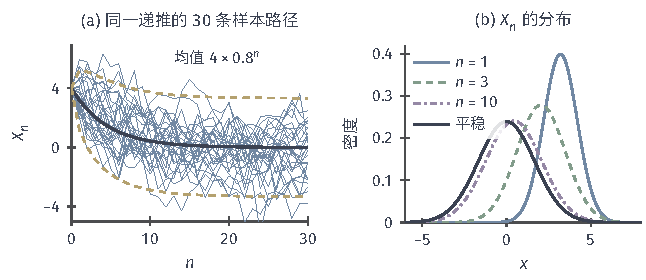
\includegraphics[width=107mm]{figures/03-optimization-evolution-and-signals/02-processes-and-trajectory-evolution/tikz/dtsp-ar1-path-bundle/figure.pdf}
  \caption{随机递推$X_{n+1}=0.8X_n+\xi_{n+1}$的路径束与边缘分布。$\xi_n$独立服从$\mathcal N(0,1)$，$X_0=4$。(a)30条模拟路径（固定随机种子），黑线为精确均值$4\times0.8^n$，黄色虚线为均值加减两倍精确标准差；(b)$n=1,3,10$时$X_n$的精确高斯密度，黑线为极限分布$\mathcal N(0,1/0.36)$。}
  \label{fig:dtsp-ar1-path-bundle}
\end{figure}

现在问：已知到时刻$n$的全部历史，下一状态的条件分布是什么？给定$\mathcal F_n=\sigma(X_0,\xi_1,\ldots,\xi_n)$后，$X_n$已经确定，而$\xi_{n+1}$与$\mathcal F_n$独立。条件期望的代入法则（可参考\BookChapterRef{chap:conditional-expectation}{卷二“条件期望与条件分布”章}）允许把已知的$X_n$当作常数代入，再对独立的$\xi_{n+1}$求平均：对每个$B\in\mathcal E$，
\begin{equation}
  \mathbb P(X_{n+1}\in B\mid\mathcal F_n)
  =\mathbb P\bigl(F(x,\xi_{1})\in B\bigr)\big|_{x=X_n}
  \qquad\text{几乎必然}.
  \label{eq:dtsp-recursion-conditional-law}
\end{equation}
右侧只通过$X_n$依赖历史。也就是说，当前状态已经把预测下一步所需的全部历史信息概括起来了。下面把这个性质单独定义，因为它不依赖于具体的递推写法。

\begin{definition}[Markov性质]
  \label{def:dtsp-markov-property}
  设过程$(X_n)_{n\geq0}$取值于$(E,\mathcal E)$并适应于滤过$(\mathcal F_n)$。若对每个$n\geq0$和每个$B\in\mathcal E$，
  \[
    \mathbb P(X_{n+1}\in B\mid\mathcal F_n)=\mathbb P(X_{n+1}\in B\mid X_n)\qquad\text{几乎必然},
  \]
  则称$(X_n)$相对于$(\mathcal F_n)$具有Markov性质，称它为\term{Markov链}（Markov chain）。未指明滤过时取自然滤过$\mathcal F_n=\sigma(X_0,\ldots,X_n)$。
\end{definition}

定义中的条件$\sigma$代数不可省略。若把滤过放大为$\mathcal G_n=\sigma(X_0,\xi_1,\ldots,\xi_{n+1})$，即提前一步知道下一份噪声，那么$X_{n+1}=F(X_n,\xi_{n+1})$对$\mathcal G_n$已经可测，它给定$\mathcal G_n$的条件分布是点质量，而给定$X_n$的条件分布仍然分散，Markov等式不再成立。同一组随机变量相对于不同的信息流可以有不同的结论；这也是第~\ref{chap:stochastic-processes-and-sample-paths}章强调先声明滤过的原因。

\paragraph{当前读数不够时扩充状态}
Markov性质是对“状态”选得是否充分的检验。考虑二阶递推
\[
  Y_{n+1}=1.2Y_n-0.5Y_{n-1}+\xi_{n+1},
\]
其中$\xi_n$独立同分布于$\mathcal N(0,1)$，并与$(Y_0,Y_1)$独立。给定$(Y_n,Y_{n-1})$时，$Y_{n+1}$的条件均值是$1.2Y_n-0.5Y_{n-1}$，显式依赖上一时刻。若$(Y_n)$本身相对于自然滤过是Markov链，给定全部历史的条件均值就只能是$Y_n$的函数；而给定$Y_n$后$Y_{n-1}$通常仍有正的条件方差，$-0.5Y_{n-1}$这一项无法写成$Y_n$的函数。因此仅记录当前读数不足以预测下一步。

补救办法是把仍然影响未来的历史放进状态。令$\bm Z_n=(Y_n,Y_{n-1})^{\top}$，则
\[
  \bm Z_{n+1}=
  \begin{pmatrix}1.2&-0.5\\1&0\end{pmatrix}\bm Z_n
  +\begin{pmatrix}\xi_{n+1}\\0\end{pmatrix},
\]
这正是式~\eqref{eq:dtsp-random-recursion}的形式，于是$(\bm Z_n)$是Markov链。相关噪声也可以这样处理：若$Y_{n+1}=0.8Y_n+\eta_{n+1}$而$\eta_{n+1}=0.5\eta_n+\xi_{n+1}$，则$(Y_n,\eta_n)$构成Markov状态。扩充状态的代价是维数增加；它把“历史依赖”改写为“高维状态的当前值依赖”，并不消除依赖本身。

\paragraph{时间齐次不等于分布不变}
在式~\eqref{eq:dtsp-random-recursion}中，更新映射$F$和噪声分布都不随$n$改变，因此每一步的条件规律相同。这种性质称为\term{时间齐次的}（time-homogeneous）。它说的是“规则不变”，而不是“分布不变”：图~\ref{fig:dtsp-ar1-path-bundle}中的递推是时间齐次的，但从$X_0=4$出发时$X_n$的均值和方差一直在变。规则不变时分布能否最终稳定、稳定到哪里，是第~\ref{sec:dtsp-long-run}节研究的问题。

\subsection{转移矩阵与转移核}
\label{sec:dtsp-kernels}

\paragraph{有限状态：转移矩阵}
先看状态有限的情形。设一台服务器每秒处于“正常”（状态$1$）或“拥堵”（状态$2$）之一。若当前正常，下一秒以$0.1$的概率变为拥堵；若当前拥堵，下一秒以$0.2$的概率恢复。把条件概率排成矩阵，
\begin{equation}
  \bm P=\begin{pmatrix}P_{1,1}&P_{1,2}\\P_{2,1}&P_{2,2}\end{pmatrix}
  =\begin{pmatrix}0.9&0.1\\0.2&0.8\end{pmatrix},
  \qquad P_{i,j}=\mathbb P(X_{n+1}=j\mid X_n=i).
  \label{eq:dtsp-two-state-matrix}
\end{equation}
图~\ref{fig:dtsp-two-state-graph}把它画成有向图：每个节点的出边概率之和为一。这条两状态链将作为全章的贯穿例子。

\begin{figure}[htbp]
  \centering
  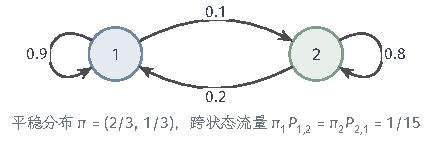
\includegraphics[width=73mm]{figures/03-optimization-evolution-and-signals/02-processes-and-trajectory-evolution/tikz/dtsp-two-state-graph/figure.pdf}
  \caption{两状态链的转移图。节点为状态，带箭头的边标出一步转移概率，自环表示停留；每个状态的出边概率之和为$1$。图下说明的平稳分布与概率流将在第~\ref{sec:dtsp-invariant}节和第~\ref{sec:dtsp-reversibility}节导出。}
  \label{fig:dtsp-two-state-graph}
\end{figure}

一般地，可数状态集$E$上的矩阵$\bm P=(P_{i,j})$若满足$P_{i,j}\geq0$且每行之和$\sum_jP_{i,j}=1$，称为\termalias{stochastic-matrix}{随机矩阵}（stochastic matrix）。时间齐次Markov链的转移矩阵就是这样的矩阵。它与初始分布$\bm\mu$一起确定一段路径的概率：
\begin{equation}
  \mathbb P(X_0=i_0,X_1=i_1,\ldots,X_n=i_n)=\mu_{i_0}P_{i_0,i_1}P_{i_1,i_2}\cdots P_{i_{n-1},i_n}.
  \label{eq:dtsp-path-probability}
\end{equation}
推导只用乘法公式：联合概率等于$\mathbb P(X_0=i_0)$依次乘以各步给定此前全部状态的条件概率，而Markov性质把第$k$个条件概率化为$P_{i_{k-1},i_k}$。例如从正常状态出发，“正常、正常、拥堵、拥堵”这段路径的概率是$1\times0.9\times0.1\times0.8=0.072$。

把式~\eqref{eq:dtsp-path-probability}对中间状态求和，就得到下一步的分布。把分布写成行向量$\bm\mu_n^{\top}=(\mathbb P(X_n=i))_{i\in E}$，则
\[
  \bm\mu_{n+1}^{\top}=\bm\mu_n^{\top}\bm P,\qquad
  \bm\mu_n^{\top}=\bm\mu_0^{\top}\bm P^n.
\]
从$\bm\mu_0=(1,0)^{\top}$出发，前两步是$(0.9,0.1)$与$(0.9\times0.9+0.1\times0.2,\;0.9\times0.1+0.1\times0.8)=(0.83,0.17)$。

\paragraph{一般状态：转移核}
状态取实数时，单点的概率通常为零，不能再列出矩阵。替代对象是对每个当前状态给出一个下一步分布的映射。

\begin{definition}[转移核]
  \label{def:dtsp-transition-kernel}
  映射$P:E\times\mathcal E\to[0,1]$若满足：对每个$x\in E$，$B\mapsto P(x,B)$是$(E,\mathcal E)$上的概率测度；对每个$B\in\mathcal E$，$x\mapsto P(x,B)$可测，则称$P$为$E$上的\term{转移核}（transition kernel）。若对所有$n\geq0$和$B\in\mathcal E$都有
  \[
    \mathbb P(X_{n+1}\in B\mid\mathcal F_n)=P(X_n,B)\qquad\text{几乎必然},
  \]
  则称$(X_n)$是相对于$(\mathcal F_n)$、以$P$为转移核的时间齐次Markov链。
\end{definition}

第一项要求说每个状态都对应一个合法的下一步分布。第二项可测性的用途在于对随机的当前状态积分：若$X_n\sim\mu_n$，则
$\mathbb P(X_{n+1}\in B)=\mathbb E[P(X_n,B)]=\int_EP(x,B)\,\mu_n(\mathrm dx)$，而这个积分只对可测函数有定义。递推~\eqref{eq:dtsp-random-recursion}给出的核是$P(x,B)=\mathbb P(F(x,\xi_1)\in B)$；在图~\ref{fig:dtsp-ar1-path-bundle}的例子中，$P(x,\cdot)=\mathcal N(0.8x,1)$。第~\ref{chap:stochastic-processes-and-sample-paths}章已经说明，给定初始分布和转移核，可以在路径空间上构造出相应的过程；本章直接使用这个过程。

\paragraph{核作用于分布与作用于函数}
同一个核有两种用法，分别对应“分布向前推”和“函数向后拉”。对概率测度$\mu$和有界可测函数$f$，定义
\begin{equation}
  (\mu P)(B)=\int_E P(x,B)\,\mu(\mathrm dx),\qquad
  Pf(x)=\int_E f(y)\,P(x,\mathrm dy).
  \label{eq:dtsp-kernel-actions}
\end{equation}
$\mu P$是从分布$\mu$出发走一步后的分布；$Pf(x)$是从$x$出发走一步后$f$的平均值，即$\mathbb E[f(X_{n+1})\mid X_n=x]$。两种作用由
\[
  (\mu P)f=\int f\,\mathrm d(\mu P)=\int Pf\,\mathrm d\mu=\mu(Pf)
\]
联系起来，等式由Fubini定理对非负或有界函数成立。有限状态时，$\mu P$是行向量乘矩阵，$Pf$是矩阵乘列向量。区分两者很有用：研究分布怎样演化时用$\mu P$，研究条件期望和鞅时用$Pf$。

\paragraph{多步转移与Chapman--Kolmogorov关系}
两个核$P,Q$的复合定义为
\[
  (PQ)(x,B)=\int_E Q(y,B)\,P(x,\mathrm dy),
\]
它表示先按$P$走一步、再按$Q$走一步。令$P^0(x,B)=\mathbb I\{x\in B\}$，$P^{m+1}=P^mP$。下面的定理说明核的幂恰好给出多步转移。

\begin{theorem}[多步转移与Chapman--Kolmogorov关系]
  \label{thm:dtsp-chapman-kolmogorov}
  设$(X_n)$是以$P$为转移核的时间齐次Markov链。则对所有$n,m\geq0$和有界可测$f$，
  \begin{equation}
    \mathbb E[f(X_{n+m})\mid\mathcal F_n]=P^mf(X_n)\qquad\text{几乎必然},
    \label{eq:dtsp-multistep}
  \end{equation}
  并且核的幂满足
  \begin{equation}
    P^{m+k}(x,B)=\int_EP^k(y,B)\,P^m(x,\mathrm dy),\qquad x\in E,\ B\in\mathcal E.
    \label{eq:dtsp-chapman-kolmogorov}
  \end{equation}
\end{theorem}

\begin{proof}
对$m$归纳证明式~\eqref{eq:dtsp-multistep}。$m=0$时两边都是$f(X_n)$。设结论对$m$成立。由塔式性质先对$\mathcal F_{n+m}$取条件期望，
\[
  \begin{aligned}
    \mathbb E[f(X_{n+m+1})\mid\mathcal F_n]
    &=\mathbb E\bigl[\mathbb E[f(X_{n+m+1})\mid\mathcal F_{n+m}]\bigm|\mathcal F_n\bigr]\\
    &=\mathbb E[Pf(X_{n+m})\mid\mathcal F_n].
  \end{aligned}
\]
第二个等号用了转移核的定义（先对指示函数成立，再由线性与单调收敛推广到有界可测$f$）。$Pf$仍有界可测，对它使用归纳假设得到$P^m(Pf)(X_n)=P^{m+1}f(X_n)$。式~\eqref{eq:dtsp-chapman-kolmogorov}是核复合的结合律：$P^{m+k}=P^mP^k$，按复合的定义展开即得。
\end{proof}

式~\eqref{eq:dtsp-chapman-kolmogorov}称为\term{Chapman--Kolmogorov关系}，它的含义是：从$x$走$m+k$步到$B$，可以先任意走$m$步到某个中间状态$y$，再从$y$走$k$步，按中间状态的分布平均。有限状态时它就是矩阵乘法$\bm P^{m+k}=\bm P^m\bm P^k$。

\paragraph{两状态链的多步分布}
对矩阵~\eqref{eq:dtsp-two-state-matrix}，可以显式算出$\bm P^n$。它的右特征向量为$(1,1)^{\top}$（特征值$1$）和$(1,-2)^{\top}$（特征值$0.7$），后者可直接验证：$\bm P(1,-2)^{\top}=(0.7,-1.4)^{\top}$。按这组特征向量展开得到
\begin{equation}
  \bm P^n=
  \begin{pmatrix}2/3&1/3\\2/3&1/3\end{pmatrix}
  +0.7^n\begin{pmatrix}1/3&-1/3\\-2/3&2/3\end{pmatrix}.
  \label{eq:dtsp-two-state-power}
\end{equation}
$n=1$时右侧确实回到$\bm P$。令$q_n=\mathbb P(X_n=2)$，一步关系为$q_{n+1}=0.1(1-q_n)+0.8q_n=0.1+0.7q_n$，于是
\[
  q_n=\frac13+0.7^n\Bigl(q_0-\frac13\Bigr).
\]
从正常状态出发，$q_1=0.1$、$q_2=0.17$、$q_{10}\approx0.324$。图~\ref{fig:dtsp-two-state-distribution}(a)画出从两个初态出发的$q_n$：两条曲线都以$0.7^n$的速度靠近$1/3$，但没有任何一步恰好等于它。式~\eqref{eq:dtsp-two-state-power}已经预告了后面几节的主题：第一项是被转移保持的分布，第二项是逐步衰减的初态影响，而衰减率$0.7=1-0.1-0.2$由两种跳转概率共同决定。

\begin{figure}[htbp]
  \centering
  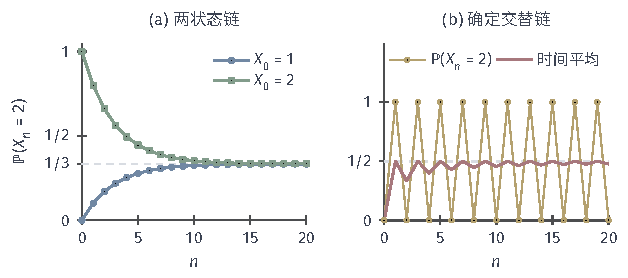
\includegraphics[width=106mm]{figures/03-optimization-evolution-and-signals/02-processes-and-trajectory-evolution/tikz/dtsp-two-state-distribution/figure.pdf}
  \caption{多步分布的两种长期表现（精确计算）。(a)两状态链~\eqref{eq:dtsp-two-state-matrix}从状态$1$和状态$2$出发时的$\mathbb P(X_n=2)=1/3+0.7^n(q_0-1/3)$，虚线为$1/3$；(b)确定交替链（$1\to2\to1\to\cdots$）从状态$1$出发时，$\mathbb P(X_n=2)$在$0,1$之间交替，红线为前$n+1$个时刻的平均，趋于$1/2$。}
  \label{fig:dtsp-two-state-distribution}
\end{figure}

\section{状态访问与不变分布}
\label{sec:dtsp-visits}

多步分布的显式公式~\eqref{eq:dtsp-two-state-power}只对很小的链可得。要判断一般链的长期行为，需要先回答三个更基本的问题：从一个状态出发能到达哪些状态，离开后是否一定回来，以及有没有一个分布被转移完整保持。本节建立这些对象和判别条件；长期分布究竟何时收敛、收敛多快，留到第~\ref{sec:dtsp-long-run}节。前两小节主要处理可数状态集$E$，记$\mathbb P_i,\mathbb E_i$为从$X_0=i$出发时的概率与期望。

\subsection{沟通、周期与回返}
\label{sec:dtsp-communication}

\paragraph{可达与沟通类}
在转移图上，若从$i$出发沿正概率的边能走到$j$，即存在$n\geq0$使$P^n(i,j)>0$，就说$j$从$i$\term{可达}（accessible），记作$i\to j$。若$i\to j$且$j\to i$，称二者\term{沟通}（communicate）。沟通关系自反（取$n=0$）、对称，并且可传递：由$P^{a+b}(i,k)\geq P^a(i,j)P^b(j,k)>0$可知。因此它把$E$分成互不相交的\term{沟通类}（communicating class）。若从一个类出发一步也离不开该类，即对类内的$i$有$\sum_{j\in C}P_{i,j}=1$，称$C$为\term{封闭类}（closed class）。整个状态集构成一个沟通类时，称链满足\term{不可约性}（irreducibility）。

图~\ref{fig:dtsp-communicating-classes}给出一个六状态的例子。状态$1,2$相互沟通，但能流向$3$或$5$，一旦离开就回不来；$\{3,4\}$和$\{5,6\}$都是封闭类。长期看，链最终会落入某个封闭类并永远留在那里，起点决定的只是落入哪一个类的概率。这说明“长期分布”首先取决于类结构：可约链的长期行为一般依赖初态。

\begin{figure}[htbp]
  \centering
  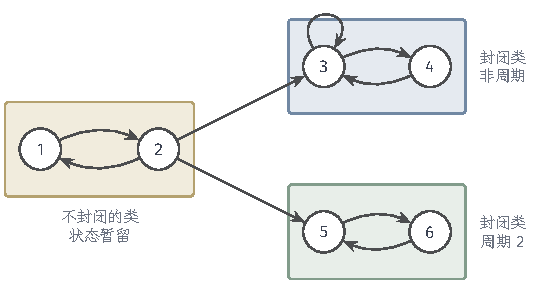
\includegraphics[width=91mm]{figures/03-optimization-evolution-and-signals/02-processes-and-trajectory-evolution/tikz/dtsp-communicating-classes/figure.pdf}
  \caption{六状态链的沟通类。箭头表示一步正概率转移（数值省略）。黄色框$\{1,2\}$不是封闭类，可以经状态$2$离开，其中状态暂留；蓝色框$\{3,4\}$与绿色框$\{5,6\}$都是封闭类，前者因状态$3$的自环而非周期，后者在$5,6$之间确定交替，周期为$2$。}
  \label{fig:dtsp-communicating-classes}
\end{figure}

\paragraph{周期}
即使所有状态互相可达，返回的时刻也可能受到限制。图~\ref{fig:dtsp-communicating-classes}的$\{5,6\}$中，从$5$出发只能在偶数步回到$5$。设$R_i=\{n\geq1:P^n(i,i)>0\}$非空，定义状态$i$的\term{周期}（period）为$d_i=\gcd R_i$。周期为$1$的状态称为非周期的。

周期是沟通类的共同性质。设$i,j$沟通，取$a,b$使$P^a(i,j)>0$、$P^b(j,i)>0$。先走$a$步到$j$再走$b$步回来，说明$a+b\in R_i$；若再在$j$处插入一段长为$n\in R_j$的回路，又有$a+n+b\in R_i$。$d_i$同时整除$a+b$与$a+n+b$，故整除每个$n\in R_j$，从而$d_i\mid d_j$。交换$i,j$得到$d_j\mid d_i$，所以$d_i=d_j$。于是可以说不可约链的周期；周期为$1$时称链是\term{非周期的}（aperiodic）。

周期链的逐时刻分布可能永远振荡。最简单的例子是确定交替链$\bm P=\left(\begin{smallmatrix}0&1\\1&0\end{smallmatrix}\right)$：每一步都合法，从状态$1$出发时$\mathbb P(X_n=2)$在$0$与$1$之间交替，见图~\ref{fig:dtsp-two-state-distribution}(b)。但同一幅图中的时间平均却趋于$1/2$。这一对照提示我们，“分布收敛”和“平均收敛”需要不同的条件；在每个状态加一个停留概率（例如改用$\frac12(\bm I+\bm P)$）就能消除周期。

\paragraph{返回概率与常返}
下面研究离开一个状态后是否一定回来。令
\[
  T_i^{+}=\inf\{n\geq1:X_n=i\},\qquad f_i=\mathbb P_i(T_i^{+}<\infty),
\]
约定空集的下确界为$\infty$。若$f_i=1$，称$i$为\term{常返状态}（recurrent state）；若$f_i<1$，称$i$为\term{暂留状态}（transient state）。

返回概率决定访问次数的分布。记$N_i=\sum_{n\geq0}\mathbb I\{X_n=i\}$为访问$i$的总次数（含时刻$0$）。每次回到$i$后，链“从$i$重新开始”，下一次能否回来与过去无关，所以
\begin{equation}
  \mathbb P_i(N_i>k)=f_i^{k},\qquad k\geq0.
  \label{eq:dtsp-visit-geometric}
\end{equation}
这里在随机的返回时刻重新开始，需要比定义~\ref{def:dtsp-markov-property}更强的强Markov性质，它将在第~\ref{sec:dtsp-strong-markov}节证明。承认这一点，常返等价于访问无穷多次，暂留时$N_i$服从几何分布，$\mathbb E_iN_i=1/(1-f_i)$。另一方面，按定义交换求和与期望，
$\mathbb E_iN_i=\sum_{n\geq0}P^n(i,i)$。两式合起来就得到一个只用转移概率的判别法：

\begin{theorem}[常返的级数判别]
  \label{thm:dtsp-recurrence-series}
  可数状态时间齐次Markov链的状态$i$常返，当且仅当$\sum_{n\geq0}P^n(i,i)=\infty$。若$i$与$j$沟通，则二者同为常返或同为暂留。
\end{theorem}

\begin{proof}
第一句由$\mathbb E_iN_i=\sum_nP^n(i,i)$与式~\eqref{eq:dtsp-visit-geometric}直接得到：$f_i<1$时期望有限，$f_i=1$时$N_i=\infty$几乎必然。对第二句，取$a,b$使$P^a(i,j)>0$、$P^b(j,i)>0$，则$P^{a+n+b}(j,j)\geq P^b(j,i)P^n(i,i)P^a(i,j)$。若$\sum_nP^n(i,i)=\infty$，右侧对$n$求和发散，所以$j$也常返；交换角色得到另一方向。
\end{proof}

\begin{example}[整数格点上的随机游走]
  \label{ex:dtsp-walk-recurrence}
  设$X_{n+1}=X_n\pm1$，向右概率为$p$，向左为$q=1-p$。回到原点必须左右步数相等，所以$P^{2n}(0,0)=\binom{2n}{n}p^nq^n$，奇数步为零。由Stirling公式，$\binom{2n}{n}\sim4^n/\sqrt{\pi n}$，因此
  \[
    P^{2n}(0,0)\sim\frac{(4pq)^n}{\sqrt{\pi n}}.
  \]
  $p=1/2$时$4pq=1$，级数如$\sum n^{-1/2}$发散，原点常返；$p\neq1/2$时$4pq<1$，级数按几何速度收敛，原点暂留。直观上，有漂移的游走以线性速度远离原点，只能回来有限次。
\end{example}

\paragraph{有限封闭类必然常返}
对有限状态链，常返性可以直接由结构判断。设$C$是有限封闭类，固定$i\in C$。对类内每个状态$j$选一条通往$i$的正概率路径；状态有限，所以存在整数$M$和$\varepsilon>0$，使从$C$中任一状态出发，在接下来$M$步内访问$i$的概率至少为$\varepsilon$。按长度为$M$的时间块反复使用Markov性质，得到
\begin{equation}
  \mathbb P_i(T_i^{+}>kM)\leq(1-\varepsilon)^k,\qquad
  \mathbb E_iT_i^{+}=\sum_{n\geq0}\mathbb P_i(T_i^{+}>n)\leq\frac{M}{\varepsilon}<\infty.
  \label{eq:dtsp-finite-return-bound}
\end{equation}
所以有限封闭类中的状态都常返，而且平均返回时间有限。不封闭的类则一定暂留：从中能以正概率走到不能返回的地方。

\paragraph{正常返与零常返}
常返只保证回来，不保证回来得快。记平均返回时间$m_i=\mathbb E_iT_i^{+}$。常返且$m_i<\infty$称\term{正常返}（positive recurrent），常返而$m_i=\infty$称\term{零常返}（null recurrent）。有限封闭类由式~\eqref{eq:dtsp-finite-return-bound}是正常返的；例~\ref{ex:dtsp-walk-recurrence}中的对称游走则是零常返，第~\ref{sec:dtsp-optional-sampling}节将用停时计算证明它从$1$首次到达$0$的期望时间为无穷。两者的差别会在长期平均中显现：第~\ref{sec:dtsp-ergodic-averages}节将证明，正常返状态$i$在长期中被访问的时间比例是$1/m_i$，零常返状态的这一比例为零。

\paragraph{一般状态空间的回返}
状态连续时，单点通常被访问的概率为零，“每个状态互相可达”不再合适，需要换成“每个有正质量的集合都能到达”。固定$(E,\mathcal E)$上的非零测度$\varphi$。若对每个满足$\varphi(B)>0$的$B$和每个初态$x$，链都以正概率在有限时间内进入$B$，称链是$\varphi$不可约的。在此基础上，\term{Harris常返性}（Harris recurrence）要求每个这样的$B$都从每个初态出发几乎必然被访问无穷多次；若再存在不变概率分布，称为\term{正Harris常返性}（positive Harris recurrence）。“以正概率到达”与“几乎必然无穷多次访问”是不同的要求：前者仍允许链以正概率逃离后永不返回。第~\ref{sec:dtsp-long-run}节的一般状态空间结论都以这类回返条件为入口\scite{math-meyn2009markov}。

\subsection{不变分布与平衡方程}
\label{sec:dtsp-invariant}

\paragraph{分布更新的不动点}
第~\ref{sec:dtsp-kernels}节把一步转移写成分布到分布的映射$\mu\mapsto\mu P$。长期问题的第一个候选答案是这个映射的不动点：从它出发走一步，各事件的概率都不变。注意不动的是分布，不是单条路径；路径仍在不停跳动，只是整体比例保持。

\begin{definition}[不变分布]
  \label{def:dtsp-invariant-distribution}
  转移核$P$的概率测度$\pi$若满足$\pi P=\pi$，即
  \[
    \pi(B)=\int_EP(x,B)\,\pi(\mathrm dx),\qquad B\in\mathcal E,
  \]
  则称$\pi$为$P$的\term{不变分布}（invariant distribution），也称\term{平稳分布}（stationary distribution）。满足同一方程、但总质量可以无穷的非负测度称为不变测度。
\end{definition}

有限状态时，不变分布是线性方程组$\bm\pi^{\top}(\bm I-\bm P)=\bm0^{\top}$在约束$\pi_i\geq0$、$\sum_i\pi_i=1$下的解，方程组的每一行说明流入状态$j$的总概率等于$j$原有的概率。对两状态链~\eqref{eq:dtsp-two-state-matrix}，第一行化为$0.1\pi_1=0.2\pi_2$，再归一化得$\bm\pi=(2/3,1/3)$，与式~\eqref{eq:dtsp-two-state-power}的第一项一致。对三状态链
\[
  \bm P=\begin{pmatrix}1/2&1/2&0\\1/4&1/2&1/4\\0&1/2&1/2\end{pmatrix},
\]
解得$\bm\pi=(1/4,1/2,1/4)$；例如第二列给出$\frac14\cdot\frac12+\frac12\cdot\frac12+\frac14\cdot\frac12=\frac12$。

非负与归一化两项条件都不可省略。对例~\ref{ex:dtsp-walk-recurrence}中的对称游走，计数测度$\pi_i=1$满足$\pi P=\pi$，因为每个格点从两侧各接收$1/2$；但它总质量无穷，不能归一化，所以对称游走没有不变分布。可约链的平衡方程又可能有多维解空间，其中包含正负相消的向量，它们满足方程却不是分布。

\paragraph{存在与唯一}
下面的定理回答有限链何时有、以及只有一个不变分布。

\begin{theorem}[有限链的不变分布]
  \label{thm:dtsp-finite-invariant}
  有限状态转移矩阵$\bm P$至少有一个不变分布。若$\bm P$不可约，则不变分布唯一，且每个分量都严格为正。
\end{theorem}

\begin{proof}
存在性：任取初始概率向量$\bm\nu$，考虑Ces\`aro平均$\bm a_n^{\top}=n^{-1}\sum_{k=0}^{n-1}\bm\nu^{\top}\bm P^k$。它们都在有限维概率单纯形中，单纯形是紧集，所以有收敛子列$\bm a_{n_\ell}\to\bm\pi$。又
\[
  \bm a_n^{\top}\bm P-\bm a_n^{\top}=\frac{\bm\nu^{\top}\bm P^n-\bm\nu^{\top}}{n},
\]
其各分量绝对值不超过$2/n$，沿子列取极限得到$\bm\pi^{\top}\bm P=\bm\pi^{\top}$。

正性：设$\bm\pi$是非零非负的不变向量而$\pi_j=0$。由$\pi_j=\sum_i\pi_iP^n(i,j)$，凡能在若干步到达$j$的状态$i$都必须有$\pi_i=0$。不可约时所有状态都能到达$j$，于是$\bm\pi=\bm0$，矛盾。

唯一性：设$\bm\pi,\bm\rho$都是不变分布，令$c=\min_j\pi_j/\rho_j>0$。向量$\bm\pi-c\bm\rho$满足平衡方程、非负，并且至少有一个分量为零；由正性的论证它只能是零向量。两边求和得$c=1$，所以$\bm\pi=\bm\rho$。
\end{proof}

可数状态的不可约链情况更细：不变分布存在当且仅当链是正常返的，此时它唯一，并且$\pi_i=1/m_i$。有限情形的这个公式将在第~\ref{sec:dtsp-ergodic-averages}节由返回分段直接证明；一般可数情形的证明思路相同\scite{math-kallenberg2021probability}。对称游走零常返，与上面“计数测度不能归一化”的观察一致。

\paragraph{存在、唯一与收敛是三件事}
不变分布回答“什么分布被保持”，并没有回答“从别处出发能否到达它”。两个例子把这几件事分开。恒等转移$\bm P=\bm I$保持每一个分布，不变分布不唯一，而且链永远不忘记初态。确定交替链不可约，唯一的不变分布是$(1/2,1/2)$，但从状态$1$出发时逐时刻分布永远在两点间交替，见图~\ref{fig:dtsp-two-state-distribution}(b)。因此在存在与唯一之外，还要有额外条件才能让初态影响消退；第~\ref{sec:dtsp-distribution-convergence}节将证明非周期性正是有限链所缺的那一项。

\subsection{可逆性与细致平衡}
\label{sec:dtsp-reversibility}

\paragraph{正放与倒放}
设想把一条从不变分布启动的链拍成录像，然后倒着播放。对两状态链，倒放的录像与正放在统计上无法区分吗？要回答这个问题，比较正向与反向路径的概率。若对每个$n$，$(X_0,X_1,\ldots,X_n)$与$(X_n,X_{n-1},\ldots,X_0)$同分布，称平稳链是\term{可逆的}（reversible）。取$n=1$，可逆性要求$\mathbb P(X_0=i,X_1=j)=\mathbb P(X_0=j,X_1=i)$，也就是从$i$流向$j$的概率流量等于反向流量。这一条件有自己的名字。

\begin{definition}[细致平衡]
  \label{def:dtsp-detailed-balance}
  概率测度$\pi$与转移核$P$满足\term{细致平衡}（detailed balance），若$E\times E$上的两个测度相等：
  \begin{equation}
    \pi(\mathrm dx)P(x,\mathrm dy)=\pi(\mathrm dy)P(y,\mathrm dx).
    \label{eq:dtsp-detailed-balance}
  \end{equation}
  可数状态时它化为$\pi_iP_{i,j}=\pi_jP_{j,i}$对所有$i,j$成立。
\end{definition}

\begin{theorem}[细致平衡、不变性与可逆性]
  \label{thm:dtsp-detailed-balance}
  若$\pi$与$P$满足细致平衡，则$\pi$是$P$的不变分布，并且从$\pi$启动的链是可逆的。反之，可逆的平稳链满足细致平衡。
\end{theorem}

\begin{proof}
对式~\eqref{eq:dtsp-detailed-balance}在$x\in E$上积分，左侧得$(\pi P)(\mathrm dy)$，右侧得$\pi(\mathrm dy)P(y,E)=\pi(\mathrm dy)$，所以$\pi P=\pi$。可数状态下验证可逆性：由式~\eqref{eq:dtsp-path-probability}，
\[
  \begin{aligned}
    \pi_{i_0}P_{i_0,i_1}P_{i_1,i_2}\cdots P_{i_{n-1},i_n}
    &=P_{i_1,i_0}\,\pi_{i_1}P_{i_1,i_2}\cdots P_{i_{n-1},i_n}\\
    &=\cdots
    =\pi_{i_n}P_{i_n,i_{n-1}}\cdots P_{i_1,i_0},
  \end{aligned}
\]
每一步用一次细致平衡把$\pi$向右移动一格。左端是正向路径的概率，右端是反向路径的概率。一般状态空间用同样的逐步换序处理有限维分布。反方向已由$n=1$的情形说明。
\end{proof}

细致平衡是一组逐对的局部等式，比整体平衡方程容易验证，也容易用来设计转移。两状态链满足它：两条跨状态流量都是$\frac23\times0.1=\frac13\times0.2=\frac1{15}$。上面的三状态链也满足它，每条边两方向的流量都是$1/8$，见图~\ref{fig:dtsp-balance-cycles}(a)。更一般地，在带非负对称边权$w_{i,j}$的图上按$P_{i,j}=w_{i,j}/w_i$随机行走（$w_i=\sum_jw_{i,j}$），取$\pi_i\propto w_i$，便有$\pi_iP_{i,j}\propto w_{i,j}=w_{j,i}\propto\pi_jP_{j,i}$，所以加权图上的随机游走都是可逆的。

\paragraph{平衡不等于细致平衡}
不变分布只要求每个状态的流入总量等于流出总量，并不要求逐边对消。图~\ref{fig:dtsp-balance-cycles}(b)中的三个状态排成一个有向环，每步以$2/3$的概率前进、以$1/3$的概率停留。均匀分布是不变的，因为每个状态从前一个状态接收$\frac13\times\frac23=\frac29$，同时向下一个状态送出同样多；但反方向的流量为零，细致平衡不成立。倒放这条链的录像，会看到它朝相反方向绕圈，一眼就能分辨。

\begin{figure}[htbp]
  \centering
  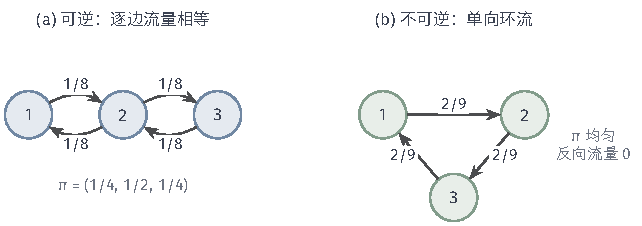
\includegraphics[width=107mm]{figures/03-optimization-evolution-and-signals/02-processes-and-trajectory-evolution/tikz/dtsp-balance-cycles/figure.pdf}
  \caption{细致平衡与整体平衡。边上的数字是平稳运行时一步的概率流量$\pi_iP_{i,j}$。(a)三状态生灭链，$\pi=(1/4,1/2,1/4)$，每条边正反流量都是$1/8$；(b)有向三循环，每步以$2/3$前进、以$1/3$停留（停留流量未画出），均匀分布不变，但只有单向流量$2/9$。}
  \label{fig:dtsp-balance-cycles}
\end{figure}

环路给出一个检验细致平衡的必要条件。若$\pi_iP_{i,j}=\pi_jP_{j,i}$对环路$1\to2\to3\to1$的三条边都成立，把三式相乘、约去$\pi_1\pi_2\pi_3$，就得到$P_{1,2}P_{2,3}P_{3,1}=P_{1,3}P_{3,2}P_{2,1}$：沿环路正走与反走的概率乘积必须相等。有向环中左侧为$(2/3)^3$，右侧为零，所以它不可逆。可逆性因此是一种额外结构，而不是不变分布的必然伴随物。第~\ref{sec:dtsp-mcmc}节将利用细致平衡这一容易验证的充分条件，设计以指定分布为不变分布的采样链。

\section{历史条件下的随机累计}
\label{sec:dtsp-accumulation}

前两节研究完整的条件分布：给定现在，未来怎样分布。很多问题只需要更少的信息。赌徒关心每局的期望输赢，算法关心每步更新平均朝哪里走，误差分析关心累计波动有多大。本节把注意力从条件分布转向条件均值，把每一步增量拆成两部分：一部分在增量出现之前就可以由历史预测，称为漂移；另一部分给定历史后平均为零，是无法用过去消除的噪声。只含后者的累计量就是鞅，它是后面停止、偏差控制与收敛分析的共同对象。

\subsection{鞅、次鞅与超鞅}
\label{sec:dtsp-martingales}

\paragraph{公平游戏的数学表达}
设$\xi_1,\xi_2,\ldots$独立，各以$1/2$的概率取$\pm1$，令$S_0=0$、$S_n=\sum_{k=1}^n\xi_k$，滤过取$\mathcal F_n=\sigma(\xi_1,\ldots,\xi_n)$。把$S_n$看成反复押一元硬币的累计输赢。无论之前赢了多少，下一局的条件期望输赢都是零：
\[
  \mathbb E[S_{n+1}\mid\mathcal F_n]=S_n+\mathbb E[\xi_{n+1}\mid\mathcal F_n]=S_n+\mathbb E\xi_{n+1}=S_n.
\]
第二个等号用了$\xi_{n+1}$与$\mathcal F_n$独立。“已知到现在为止的一切，对下一时刻的最佳平均预测就是现在的值”，这就是公平游戏的数学表达。

\begin{definition}[鞅、次鞅与超鞅]
  \label{def:dtsp-martingale}
  设实值过程$(M_n)_{n\geq0}$适应于滤过$(\mathcal F_n)$，且每个$M_n$可积。若对所有$n\geq0$，
  \begin{equation}
    \mathbb E[M_{n+1}\mid\mathcal F_n]=M_n\qquad\text{几乎必然},
    \label{eq:dtsp-martingale}
  \end{equation}
  则称$(M_n)$为相对于$(\mathcal F_n)$的\term{鞅}（martingale）。若等号换成“$\geq$”，称为\term{次鞅}（submartingale）；换成“$\leq$”，称为\term{超鞅}（supermartingale）。鞅的增量$D_n=M_n-M_{n-1}$满足$\mathbb E[D_n\mid\mathcal F_{n-1}]=0$，称为\term{鞅差}（martingale difference）。
\end{definition}

可积性保证条件期望有定义，适应性保证$M_n$在时刻$n$已经可知。反复使用塔式性质，式~\eqref{eq:dtsp-martingale}推出$\mathbb E[M_{n+k}\mid\mathcal F_n]=M_n$对所有$k\geq0$成立，特别地$\mathbb EM_n=\mathbb EM_0$：鞅的期望不随时间改变。次鞅的期望单调不减，超鞅的期望单调不增。名称容易记反：超鞅“平均向下”，像对赌徒不利的赌场；次鞅“平均向上”。

\paragraph{几个基本例子}
下面的例子在后文会反复出现，每个都对应一种构造鞅的方式。
\begin{enumerate}
  \item 中心化累计和。若$\xi_k$独立可积、均值为$\mu$，则$S_n-n\mu$是鞅。向右概率为$p$的$\pm1$游走中$\mu=2p-1$；$p<1/2$时$S_n$本身是超鞅。
  \item 乘积。若$Y_k\geq0$独立且$\mathbb EY_k=1$，则$M_n=\prod_{k=1}^nY_k$是鞅，因为$\mathbb E[M_{n+1}\mid\mathcal F_n]=M_n\mathbb EY_{n+1}$。取$Y_k$等概率为$0$或$2$，得到“加倍或清零”的赌局，它将在第~\ref{sec:dtsp-martingale-limits}节说明鞅的极限与期望可以分离。
  \item 信息逐步揭示。若$Z$可积，则$M_n=\mathbb E[Z\mid\mathcal F_n]$是鞅，由塔式性质直接验证。它表示随信息增加不断修正的最佳预测，称为Doob鞅。
  \item 凸函数。若$(M_n)$是鞅、$\varphi$凸且$\varphi(M_n)$可积，条件Jensen不等式给出$\mathbb E[\varphi(M_{n+1})\mid\mathcal F_n]\geq\varphi(M_n)$，所以$\varphi(M_n)$是次鞅。例如$S_n^2$与$|S_n|$都是次鞅。
\end{enumerate}

\paragraph{信息流决定鞅性质}
鞅的定义中出现了$\mathcal F_n$，结论因此依赖声明的信息流。对上面的公平游走，若改用提前一步揭晓的滤过$\mathcal G_n=\sigma(\xi_1,\ldots,\xi_{n+1})$，$S_n$仍然适应，但$\mathbb E[S_{n+1}\mid\mathcal G_n]=S_{n+1}$，通常不等于$S_n$。偷看下一枚硬币的人眼中，这场游戏不再公平。反过来，若一个过程相对于较细的滤过是鞅，那么相对于它自己生成的较粗滤过仍是鞅：对较粗的信息再取一次条件期望即可。

\paragraph{Markov性质与鞅性质的比较}
Markov性质与鞅性质约束不同的对象。前者说给定现在后，未来的整个条件分布不再依赖过去；后者只说下一步的条件均值等于现在。公平游走二者兼有。有漂移的游走与递推~\eqref{eq:dtsp-random-recursion}是Markov链但不是鞅，因为它们的条件均值偏离当前值。反过来，鞅也不必是Markov链：令下注额$H_k=1+|S_{k-1}|$，累计财富$W_n=\sum_{k=1}^nH_k\xi_k$。给定$\mathcal F_n$，下一步是$W_n\pm(1+|S_n|)$，均值为$W_n$，所以$(W_n)$是鞅；但这一条件分布依赖$S_n$，而$S_n$一般不能由$W_n$确定，因此$(W_n)$相对于$(\mathcal F_n)$不是Markov链。鞅性质只管平均，允许波动的大小依赖整段历史。

\subsection{可预测加权与漂移分解}
\label{sec:dtsp-predictable}

\paragraph{鞅变换：事前下注}
赌徒可以根据已有结果改变每局下注额。关键的限制是：第$k$局的下注额必须在这一局开出之前决定。把这一要求写成可测性：若对每个$k\geq1$，$H_k$对$\mathcal F_{k-1}$可测，就称$(H_k)$是\term{可预测过程}（predictable process）。“可预测”不是说$H_k$没有随机性，而是说它可以由第$k$份新噪声到来之前的信息确定。按此下注的累计收益
\begin{equation}
  (H\cdot M)_n=\sum_{k=1}^nH_k(M_k-M_{k-1})
  \label{eq:dtsp-martingale-transform}
\end{equation}
称为\term{鞅变换}（martingale transform）。它是“随机和”的离散版本：权重在增量揭晓之前确定。

\begin{theorem}[鞅变换]
  \label{thm:dtsp-martingale-transform}
  设$(M_n)$是鞅，$(H_k)$可预测，并且每个$H_k(M_k-M_{k-1})$可积（例如每个$H_k$有界）。则$((H\cdot M)_n)_{n\geq0}$是鞅，其中$(H\cdot M)_0=0$。若$(M_n)$是超鞅，$H_k$非负且有界，则$(H\cdot M)$是超鞅。
\end{theorem}

\begin{proof}
$(H\cdot M)_n$适应且可积。由于$H_{n+1}$对$\mathcal F_n$可测，条件期望可以把它当作已知因子提出：
\[
  \mathbb E[(H\cdot M)_{n+1}-(H\cdot M)_n\mid\mathcal F_n]
  =H_{n+1}\,\mathbb E[M_{n+1}-M_n\mid\mathcal F_n].
\]
鞅情形右侧为零。超鞅情形条件期望非正，再乘以非负的$H_{n+1}$仍非正。
\end{proof}

这个定理说的是：在公平游戏中，不存在只依赖过去的下注系统能把期望收益变为正数。图~\ref{fig:dtsp-martingale-transform}比较两种规则。“按符号跟随”在领先时押正、落后时押负，它只用过去，所以$4000$条路径的平均财富始终贴着零，第$200$局时样本平均为$-0.03$，标准误$0.23$。“事后挑选”每局押中刚揭晓的结果，$H_k=\xi_k$，财富一路涨到$n$；它违反了可预测性，证明中“把$H_{n+1}$提出条件期望”那一步失去依据。定理中的可积性同样不可省略；第~\ref{sec:dtsp-optional-sampling}节的加倍下注会说明，缺少适当的可积或有界条件时，“随机长度”的公平游戏可以产生看似必胜的结果。

\begin{figure}[htbp]
  \centering
  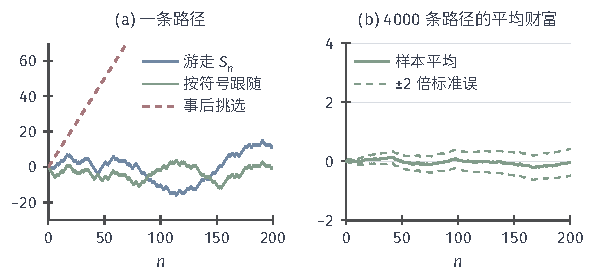
\includegraphics[width=101mm]{figures/03-optimization-evolution-and-signals/02-processes-and-trajectory-evolution/tikz/dtsp-martingale-transform/figure.pdf}
  \caption{事前下注与事后挑选。$S_n$为公平$\pm1$游走。“按符号跟随”取$H_k=\operatorname{sign}(S_{k-1})$（约定$\operatorname{sign}0=1$），只用过去；“事后挑选”取$H_k=\xi_k$，财富等于$n$。(a)一条路径；(b)$4000$条模拟路径上“按符号跟随”的平均财富及其两倍标准误带，始终覆盖零。}
  \label{fig:dtsp-martingale-transform}
\end{figure}

\paragraph{Doob分解：漂移与噪声}
一般的适应过程未必公平。它的每一步增量都可以拆成“事先可预测的平均”与“剩余的意外”。设$(X_n)$适应且可积，令
\begin{equation}
  A_n=\sum_{k=1}^{n}\mathbb E[X_k-X_{k-1}\mid\mathcal F_{k-1}],\qquad
  M_n=X_n-X_0-A_n,
  \label{eq:dtsp-doob-decomposition}
\end{equation}
并约定$A_0=M_0=0$。

\begin{theorem}[Doob分解]
  \label{thm:dtsp-doob-decomposition}
  适应可积过程$(X_n)$可以写成$X_n=X_0+M_n+A_n$，其中$(M_n)$是鞅，$(A_n)$可预测，且$M_0=A_0=0$。这种分解在几乎必然意义下唯一。$(X_n)$是次鞅当且仅当$(A_n)$单调不减；是超鞅当且仅当$(A_n)$单调不增。
\end{theorem}

\begin{proof}
按式~\eqref{eq:dtsp-doob-decomposition}构造，$A_n$的每一项对$\mathcal F_{k-1}\subseteq\mathcal F_{n-1}$可测，所以$A_n$可预测；又
\[
  \mathbb E[M_k-M_{k-1}\mid\mathcal F_{k-1}]=\mathbb E[X_k-X_{k-1}\mid\mathcal F_{k-1}]-(A_k-A_{k-1})=0,
\]
所以$M$是鞅。若另有分解$X_n=X_0+M_n'+A_n'$，则$M_n-M_n'=A_n'-A_n$既是鞅又可预测，于是$M_n-M_n'=\mathbb E[M_n-M_n'\mid\mathcal F_{n-1}]=M_{n-1}-M_{n-1}'$，归纳得它恒等于初值$0$。最后一句由$A_k-A_{k-1}=\mathbb E[X_k-X_{k-1}\mid\mathcal F_{k-1}]$的符号直接读出。
\end{proof}

以公平游走的平方为例。$\mathbb E[S_k^2-S_{k-1}^2\mid\mathcal F_{k-1}]=\mathbb E[2S_{k-1}\xi_k+\xi_k^2\mid\mathcal F_{k-1}]=1$，所以$A_n=n$、$M_n=S_n^2-n$。图~\ref{fig:dtsp-doob-decomposition}把一条路径的$S_n^2$拆成一条直线和一条围绕零波动的曲线；许多路径平均后，$S_n^2$的平均正好贴着漂移线$n$。Doob分解给出后文的标准分析路线：漂移部分用确定性的稳定性或单调性处理，鞅部分用本章后几节的累计偏差与收敛工具处理。第~\ref{sec:dtsp-stochastic-approximation}节的随机递推正是按这条路线分析的。

\begin{figure}[htbp]
  \centering
  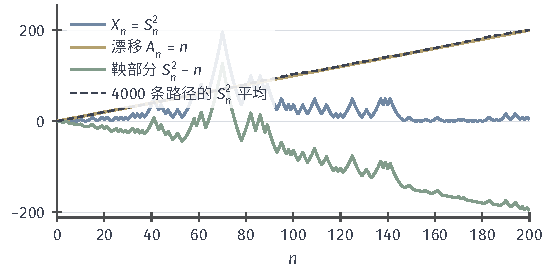
\includegraphics[width=94mm]{figures/03-optimization-evolution-and-signals/02-processes-and-trajectory-evolution/tikz/dtsp-doob-decomposition/figure.pdf}
  \caption{次鞅$S_n^2$的Doob分解。$S_n$为公平$\pm1$游走的一条模拟路径，$S_n^2=(S_n^2-n)+n$分为鞅部分（绿）与可预测漂移$A_n=n$（黄）。黑色虚线是$4000$条模拟路径上$S_n^2$的平均，与$n$几乎重合。}
  \label{fig:dtsp-doob-decomposition}
\end{figure}

\subsection{条件方差与累计波动}
\label{sec:dtsp-quadratic-variation}

\paragraph{鞅增量的正交性}
鞅的均值不变，波动却会累计。设$(M_n)$平方可积，即每个$\mathbb EM_n^2<\infty$。对$j<k$，$D_j$对$\mathcal F_{k-1}$可测，于是
\[
  \mathbb E[D_jD_k]=\mathbb E\bigl[D_j\,\mathbb E[D_k\mid\mathcal F_{k-1}]\bigr]=0.
\]
不同时刻的鞅差在$L^2$中两两正交。把$M_n=M_0+\sum_{k\leq n}D_k$平方后取期望，交叉项全部消失：
\begin{equation}
  \mathbb EM_n^2=\mathbb EM_0^2+\sum_{k=1}^n\mathbb ED_k^2.
  \label{eq:dtsp-orthogonal-increments}
\end{equation}
这是一个“勾股定理”：总长度的平方等于各段正交分量长度平方之和。对公平游走，$\mathbb ES_n^2=n$。

正交不等于独立。在“按符号跟随”或$H_k=1+|S_{k-1}|$这类下注规则中，第$k$步的幅度取决于此前的路径，增量之间显然不独立；但只要条件均值为零，式~\eqref{eq:dtsp-orthogonal-increments}照样成立。把鞅差一律当成独立同分布，会漏掉条件方差随历史变化这一最常见的情形。

\paragraph{可预测二次变差与实现二次变差}
式~\eqref{eq:dtsp-orthogonal-increments}只给出无条件的二阶矩。要描述波动怎样沿路径累计，需要逐步的条件版本。对平方可积鞅，定义
\begin{equation}
  \langle M\rangle_n=\sum_{k=1}^n\mathbb E[D_k^2\mid\mathcal F_{k-1}],\qquad
  [M]_n=\sum_{k=1}^nD_k^2.
  \label{eq:dtsp-quadratic-variations}
\end{equation}
$\langle M\rangle_n$称为\term{可预测二次变差}（predictable quadratic variation），它的每一项在第$k$步发生之前就已知，像一份预先登记的“波动预算”；$[M]_n$称为\term{实现二次变差}（realized quadratic variation），是事后数出来的平方增量之和。二者都能补偿$M_n^2$的增长：$M_n^2-\langle M\rangle_n$与$M_n^2-[M]_n$都是鞅，因为
\[
  \mathbb E[M_k^2-M_{k-1}^2\mid\mathcal F_{k-1}]=\mathbb E[2M_{k-1}D_k+D_k^2\mid\mathcal F_{k-1}]=\mathbb E[D_k^2\mid\mathcal F_{k-1}].
\]
由此，$M_n^2-M_0^2-\langle M\rangle_n$正是次鞅$M_n^2$的Doob分解中的鞅部分，而$\langle M\rangle$是它的可预测漂移。

\paragraph{为什么要跟踪条件方差}
考虑一位“领先时加大、落后时减小”的赌徒：$H_k=2$若$S_{k-1}\geq0$，否则$H_k=1/2$，财富$W_n=\sum_{k\leq n}H_k\xi_k$。由定理~\ref{thm:dtsp-martingale-transform}，$W$是鞅；它的可预测二次变差$\langle W\rangle_n=\sum_{k\leq n}H_k^2$却是随机的，可以在$n/4$与$4n$之间任意取值，取决于游走领先的时间比例。若只用最坏情形$4n$来估计$W_n$的波动，会严重高估长期落后路径上的误差；若用平均情形，又会低估长期领先的路径。第~\ref{sec:dtsp-deviation}节的Freedman不等式正是按每条路径实际累计的$\langle W\rangle_n$来控制偏差，而不是按事先固定的最坏范围。

\section{停止时刻与首次到达}
\label{sec:dtsp-stopping}
\label{sec:stoch-martingales-stopping-sequential-concentration}

很多观察不是运行固定步数后结束，而是“到某件事发生为止”：游走首次碰到边界，库存首次耗尽，算法的误差估计首次低于阈值。结束时刻因此是随机的。本节回答两个问题。第一，在随机时刻停止后，鞅的“期望不变”是否还成立，什么条件下成立；它给出到达概率和平均到达时间的计算方法。第二，Markov链在随机时刻停下后，未来是否仍像从当前状态重新开始；它是研究回返与长期平均的基础。

\subsection{停止规则与停止过程}
\label{sec:dtsp-stopping-rules}

\paragraph{只凭已有记录决定停止}
可执行的停止规则必须在每个时刻只根据已经看到的记录判断“现在停不停”。第~\ref{chap:stochastic-processes-and-sample-paths}章把这一要求写成：取值于$\mathbb N_0\cup\{\infty\}$的随机时刻$\tau$若对每个$n\geq0$都有$\{\tau\leq n\}\in\mathcal F_n$，就称为相对于$(\mathcal F_n)$的\term{停时}（stopping time），即停止时刻。离散时间中这等价于$\{\tau=n\}\in\mathcal F_n$对每个$n$成立，因为$\{\tau=n\}=\{\tau\leq n\}\setminus\{\tau\leq n-1\}$，而$\{\tau\leq n\}=\bigcup_{k\leq n}\{\tau=k\}$。

最常用的停时是首次到达。对可测集$A$，令$\tau_A=\inf\{n\geq0:X_n\in A\}$，则
\[
  \{\tau_A\leq n\}=\bigcup_{k=0}^n\{X_k\in A\}\in\mathcal F_n,
\]
到时刻$n$为止只需逐一检查已见的状态。常数时刻是停时；若$\sigma,\tau$是停时，则$\sigma\wedge\tau$、$\sigma\vee\tau$与$\tau+1$也是停时，例如$\{\sigma\wedge\tau\leq n\}=\{\sigma\leq n\}\cup\{\tau\leq n\}$。但$\tau-1$一般不是：在首次到达的前一刻宣布停止，需要预知下一步。同样，“在$0$到$N$之间路径取最大值的最后时刻”也不是停时，因为要确认某时刻之后再没有更高的值，必须看完整段路径。

\paragraph{停止过程}
在停时$\tau$处冻结一个过程，得到\term{停止过程}（stopped process）$M^{\tau}_n=M_{\tau\wedge n}$：$\tau$之前随原过程变化，之后保持在$M_\tau$不动。用鞅差写出来，
\begin{equation}
  M_{\tau\wedge n}=M_0+\sum_{k=1}^n\mathbb I\{\tau\geq k\}D_k.
  \label{eq:dtsp-stopped-process}
\end{equation}
冻结相当于从$\tau$之后把下注额设为零。由于$\{\tau\geq k\}=\{\tau\leq k-1\}^{\mathrm c}\in\mathcal F_{k-1}$，权重$H_k=\mathbb I\{\tau\geq k\}$可预测且有界，定理~\ref{thm:dtsp-martingale-transform}立即给出：鞅的停止过程仍是鞅，超鞅、次鞅的停止过程分别仍是超鞅、次鞅。冻结不破坏适应性，也不改变“每一步公平”这一性质。

\paragraph{停时处的信息}
停止以后，我们手里有哪些信息？直观上是“到$\tau$为止看到的一切”。把它写成$\sigma$代数：
\[
  \mathcal F_\tau=\{A\in\mathcal F:\ A\cap\{\tau\leq n\}\in\mathcal F_n\text{对每个}n\geq0\}.
\]
事件$A$属于$\mathcal F_\tau$，意思是在每个时刻$n$，只要已经停止，就能根据已有记录判断$A$是否发生。可以验证$\mathcal F_\tau$是$\sigma$代数；若$(X_n)$适应，则$X_\tau\mathbb I\{\tau<\infty\}$对$\mathcal F_\tau$可测，因为$\{X_\tau\in B\}\cap\{\tau=k\}=\{X_k\in B\}\cap\{\tau=k\}\in\mathcal F_k$。若$\sigma\leq\tau$，则$\mathcal F_\sigma\subseteq\mathcal F_\tau$：较早停止的人知道得较少。

\subsection{可选抽样与越界计算}
\label{sec:dtsp-optional-sampling}

\paragraph{有界停时}
既然停止过程仍是鞅，就有$\mathbb EM_{\tau\wedge n}=\mathbb EM_0$对每个固定的$n$成立。若$\tau$本身有上界$N$，取$n=N$便得到$\mathbb EM_\tau=\mathbb EM_0$。下面的定理把它推广到两个停时之间的条件期望。

\begin{theorem}[有界停时的可选抽样]
  \label{thm:dtsp-bounded-optional-sampling}
  设$(M_n)$是鞅，$\sigma\leq\tau\leq N$是两个停时，$N$为确定整数。则
  \[
    \mathbb E[M_\tau\mid\mathcal F_\sigma]=M_\sigma\qquad\text{几乎必然},
  \]
  特别地$\mathbb EM_\tau=\mathbb EM_0$。若$(M_n)$是次鞅（超鞅），等号换成$\geq$（$\leq$）。
\end{theorem}

\begin{proof}
$M_\sigma$对$\mathcal F_\sigma$可测，且$|M_\sigma|\leq\sum_{k\leq N}|M_k|$可积。只需对每个$A\in\mathcal F_\sigma$证明$\mathbb E[(M_\tau-M_\sigma)\mathbb I_A]=0$。由于$\sigma\leq\tau\leq N$，
\[
  (M_\tau-M_\sigma)\mathbb I_A=\sum_{k=1}^N\mathbb I_A\mathbb I\{\sigma<k\leq\tau\}D_k
  =\sum_{k=1}^N\mathbb I_{A\cap\{\sigma\leq k-1\}}\mathbb I\{\tau\geq k\}D_k.
\]
按$\mathcal F_\sigma$的定义，$A\cap\{\sigma\leq k-1\}\in\mathcal F_{k-1}$；又$\{\tau\geq k\}\in\mathcal F_{k-1}$。每一项的系数对$\mathcal F_{k-1}$可测，取期望后由$\mathbb E[D_k\mid\mathcal F_{k-1}]=0$为零。次鞅与超鞅情形中$\mathbb E[D_k\mid\mathcal F_{k-1}]$分别非负、非正，系数非负，得到相应不等式。
\end{proof}

证明清楚地标出了有界性的用途：它把随机长度的和改写成固定的有限和，从而可以逐项取期望。

\paragraph{从有界到无界：截断与极限交换}
实际的停时往往无界，例如“首次到达$1$”可能需要任意多步。自然的做法是先截断，再取极限：$\tau\wedge n$有界，所以$\mathbb EM_{\tau\wedge n}=\mathbb EM_0$；若$\tau<\infty$几乎必然，则$M_{\tau\wedge n}\to M_\tau$几乎必然。问题在于期望与极限能否交换。卷二已经建立了几乎处处收敛、依概率收敛与平均收敛的关系，控制收敛定理，一致可积条件下期望极限的交换，以及独立同分布序列的强大数律（可参考\BookChapterRef{chap:random-variable-convergence}{卷二“随机变量的收敛与积分极限”章}）。本章在这里和第~\ref{sec:dtsp-martingale-limits}、\ref{sec:dtsp-ergodic-averages}、\ref{sec:dtsp-iid-sampling}节调用这些结论。

\begin{theorem}[可选停止]
  \label{thm:dtsp-optional-stopping}
  设$(M_n)$是鞅，$\tau$是几乎必然有限的停时。若下列条件之一成立，则$M_\tau$可积且$\mathbb EM_\tau=\mathbb EM_0$：
  \begin{enumerate}
    \item 存在可积随机变量$Y$，使$|M_{\tau\wedge n}|\leq Y$对所有$n$成立；
    \item $\mathbb E\tau<\infty$，且存在常数$c$使$\mathbb E[|D_k|\mid\mathcal F_{k-1}]\leq c$对所有$k$成立；
    \item 停止过程$(M_{\tau\wedge n})_{n\geq0}$一致可积。
  \end{enumerate}
\end{theorem}

\begin{proof}
在每种条件下都从$\mathbb EM_{\tau\wedge n}=\mathbb EM_0$及$M_{\tau\wedge n}\to M_\tau$几乎必然出发。条件1下用控制收敛定理，条件3下用一致可积条件下的平均收敛，均得$\mathbb EM_{\tau\wedge n}\to\mathbb EM_\tau$。条件2化为条件1：取$Y=|M_0|+\sum_{k=1}^{\tau}|D_k|$，则$|M_{\tau\wedge n}|\leq Y$，且由非负项的换序与塔式性质，
\[
  \begin{aligned}
    \mathbb E\sum_{k=1}^{\tau}|D_k|&=\sum_{k\geq1}\mathbb E\bigl[\mathbb I\{\tau\geq k\}\,\mathbb E[|D_k|\mid\mathcal F_{k-1}]\bigr]\\
    &\leq c\sum_{k\geq1}\mathbb P(\tau\geq k)=c\,\mathbb E\tau<\infty.
  \end{aligned}
\]
这里$\{\tau\geq k\}\in\mathcal F_{k-1}$保证可以先对$D_k$取条件期望。
\end{proof}

三个条件从不同方向排除同一种危险：停止前的路径可能偏得极远，虽然概率很小，却把期望拉走了。只知道$\tau<\infty$几乎必然并不够。从$0$出发的公平游走，令$\tau=\inf\{n:S_n=1\}$。下面马上会证明$\tau<\infty$几乎必然，于是$S_\tau=1$，$\mathbb ES_\tau=1\neq0=\mathbb ES_0$。三个条件都不成立：$S_{\tau\wedge n}$向下无界，$\mathbb E\tau=\infty$，停止过程也不一致可积。

\paragraph{赌徒破产：到达概率与平均时间}
把游走限制在有界区间里，可选停止就成为计算工具。设$\pm1$游走向右概率为$p$、向左为$q=1-p$，从$k\in\{0,1,\ldots,N\}$出发，$\tau$为首次到达$0$或$N$的时刻。

第一步是确认$\mathbb E\tau<\infty$。从区间内任一点出发，连续向右$N$步必然离开区间，其概率为$p^N$。按长度$N$分块，每块独立地以至少$p^N$的概率结束，所以$\mathbb P(\tau>jN)\leq(1-p^N)^j$，$\mathbb E\tau\leq N/p^N<\infty$。

公平情形$p=1/2$。$S_n$是鞅，停止过程夹在$0$与$N$之间，条件1成立，于是$k=\mathbb ES_\tau=N\,\mathbb P_k(S_\tau=N)$，
\begin{equation}
  \mathbb P_k(\text{先到}N)=\frac kN.
  \label{eq:dtsp-ruin-fair}
\end{equation}
再用鞅$S_n^2-n$求平均时间。由有界停时的结论，$\mathbb E[S_{\tau\wedge n}^2]=k^2+\mathbb E[\tau\wedge n]$。令$n\to\infty$，左侧由有界收敛趋于$\mathbb ES_\tau^2=N^2\cdot k/N$，右侧由单调收敛趋于$k^2+\mathbb E\tau$，所以
\[
  \mathbb E_k\tau=k(N-k).
\]
从$N=10$的中点$k=5$出发平均需要$25$步，从$k=3$出发需要$21$步。

有漂移的情形$p\neq1/2$。$S_n$不再是鞅，但令$r=q/p$，乘积型过程$r^{S_n}$是鞅：$\mathbb E[r^{S_{n+1}}\mid\mathcal F_n]=r^{S_n}(pr+qr^{-1})=r^{S_n}(q+p)=r^{S_n}$。它在区间上有界，可选停止给出$r^k=\mathbb P_k(\text{先到}N)\,r^N+(1-\mathbb P_k(\text{先到}N))$，即
\begin{equation}
  \mathbb P_k(\text{先到}N)=\frac{1-r^k}{1-r^N}.
  \label{eq:dtsp-ruin-biased}
\end{equation}
取$N=10$、$k=3$、$p=0.47$，$r\approx1.128$，到达$10$的概率约为$0.187$，而公平时为$0.3$：每步$3\%$的劣势在十格的区间上被放大。图~\ref{fig:dtsp-gamblers-ruin}(b)把式~\eqref{eq:dtsp-ruin-fair}与\eqref{eq:dtsp-ruin-biased}同每个起点$4000$次模拟的频率放在一起。平均时间可用鞅$S_n-n(p-q)$同样求出：$\mathbb E_k\tau=(\mathbb E_kS_\tau-k)/(p-q)$。

\begin{figure}[htbp]
  \centering
  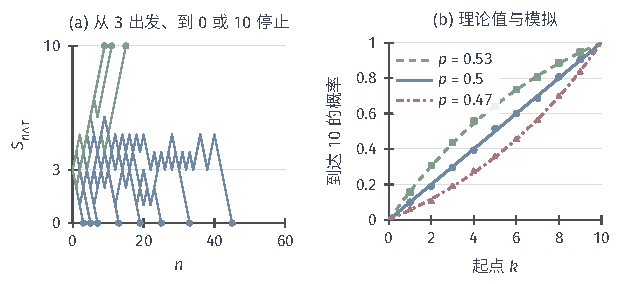
\includegraphics[width=105mm]{figures/03-optimization-evolution-and-signals/02-processes-and-trajectory-evolution/tikz/dtsp-gamblers-ruin/figure.pdf}
  \caption{赌徒破产问题。(a)公平游走从$3$出发、在首次到达$0$或$10$时停止的$14$条模拟路径（只画出$60$步内停止的路径），绿色为先到$10$；(b)先到$10$的概率随起点$k$的变化，曲线为式~\eqref{eq:dtsp-ruin-fair}与\eqref{eq:dtsp-ruin-biased}的精确值，标记为每个起点$4000$次模拟的频率。}
  \label{fig:dtsp-gamblers-ruin}
\end{figure}

\paragraph{首次到达的无界情形}
现在回到无界区间。公平游走从$0$出发，令$\sigma_m$为首次到达$1$或$-m$的时刻。由式~\eqref{eq:dtsp-ruin-fair}（把区间平移到$\{0,\ldots,m+1\}$，起点为$m$），先到$1$的概率是$m/(m+1)$，平均时间是$m\cdot1=m$。令$m\to\infty$：首次到达$1$的时刻$\tau$满足$\mathbb P(\tau<\infty)\geq m/(m+1)$对所有$m$成立，所以$\tau<\infty$几乎必然；又$\tau\geq\sigma_m$，故$\mathbb E\tau\geq m$对所有$m$成立，$\mathbb E\tau=\infty$。由对称性，从$1$出发首次回到$0$的时间期望也无穷，因此原点的平均返回时间$m_0=1+\mathbb E_1\tau_0=\infty$。这兑现了第~\ref{sec:dtsp-communication}节的说法：对称游走常返，但是零常返。

\paragraph{加倍下注：缺少条件的停止策略}
“公平游戏可以随意停止而仍然公平”并不是无条件的命题，加倍下注是最有名的反例。赌徒第一局押$1$，输了就把赌注加倍，直到第一次赢为止。若首胜出现在第$k$局，此前输掉$1+2+\cdots+2^{k-2}=2^{k-1}-1$，最后赢回$2^{k-1}$，净赢$1$。首胜几乎必然出现，所以$W_\tau=1$几乎必然，看起来是稳赚的系统。

矛盾出在哪里？每个截断时刻$n$，$W_{\tau\wedge n}$都是有界停时处的鞅值，期望为零。把它拆成已停与未停两部分：
\[
  \mathbb EW_{\tau\wedge n}=\underbrace{1\cdot\mathbb P(\tau\leq n)}_{1-2^{-n}}+\underbrace{(-(2^n-1))\cdot\mathbb P(\tau>n)}_{-(1-2^{-n})}=0.
\]
图~\ref{fig:dtsp-doubling-strategy}(b)画出这两项：未停部分的概率$2^{-n}$趋于零，它对期望的贡献却始终接近$-1$。极限中这份负质量“跑到了无穷远”，所以$\lim_n\mathbb EW_{\tau\wedge n}=0\neq1=\mathbb EW_\tau$。定理~\ref{thm:dtsp-optional-stopping}的三个条件都失败：亏损无下界，$\mathbb E\sum_{k\leq\tau}|D_k|=\sum_k2^{k-1}\cdot2^{-(k-1)}=\infty$，停止过程不一致可积。若赌徒有信用上限，最多连输$m$局，那么停止时刻有界为$m$，期望收益严格为零：以概率$1-2^{-m}$赢$1$，以概率$2^{-m}$输$2^m-1$。

\begin{figure}[htbp]
  \centering
  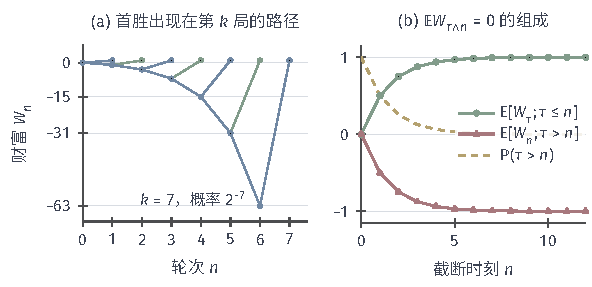
\includegraphics[width=100mm]{figures/03-optimization-evolution-and-signals/02-processes-and-trajectory-evolution/tikz/dtsp-doubling-strategy/figure.pdf}
  \caption{加倍下注（精确计算）。(a)首胜出现在第$k=1,\ldots,7$局时的财富路径，每条路径的概率为$2^{-k}$，终点都是$+1$；(b)截断期望$\mathbb EW_{\tau\wedge n}=0$的两个组成部分：已停部分$\mathbb E[W_\tau;\tau\leq n]=1-2^{-n}$与未停部分$\mathbb E[W_n;\tau>n]=-(1-2^{-n})$，以及未停概率$2^{-n}$。}
  \label{fig:dtsp-doubling-strategy}
\end{figure}

\subsection{停止后的Markov链}
\label{sec:dtsp-strong-markov}

\paragraph{强Markov性质}
可选抽样处理的是期望；现在研究停止后整个未来的条件分布。Markov性质说，在固定时刻$n$给定现在，未来像从$X_n$重新出发的链。若把$n$换成停时$\tau$，结论是否仍成立？对离散时间链，答案是肯定的，而且证明只需按$\tau$的取值拆开。记$\mathbb E_x$为从$x$出发、以$P$为转移核的链的期望，并先把定理~\ref{thm:dtsp-chapman-kolmogorov}推广到路径函数：对有界可测$g$，
\begin{equation}
  \mathbb E[g(X_n,X_{n+1},\ldots,X_{n+m})\mid\mathcal F_n]=\mathbb E_{X_n}[g(X_0,\ldots,X_m)]\qquad\text{几乎必然}.
  \label{eq:dtsp-markov-path}
\end{equation}
对乘积形式$g=\prod_jg_j(x_j)$，它由对$m$归纳、每次用一步转移核得到；一般的有界可测$g$再由单调类论证推出。

\begin{theorem}[离散时间的强Markov性质]
  \label{thm:dtsp-strong-markov}
  设$(X_n)$是以$P$为转移核的时间齐次Markov链，$\tau$是停时。则对每个$A\in\mathcal F_\tau$、每个$m\geq0$和每个有界可测$g$，
  \[
    \mathbb E\bigl[g(X_\tau,\ldots,X_{\tau+m})\,\mathbb I_A\,\mathbb I\{\tau<\infty\}\bigr]
    =\mathbb E\bigl[\mathbb E_{X_\tau}[g(X_0,\ldots,X_m)]\,\mathbb I_A\,\mathbb I\{\tau<\infty\}\bigr].
  \]
  也就是说，在$\{\tau<\infty\}$上给定$\mathcal F_\tau$，停止后的过程$(X_{\tau+n})_{n\geq0}$是从$X_\tau$出发、以$P$为转移核的Markov链。
\end{theorem}

\begin{proof}
把左侧按$\{\tau=n\}$拆成可数和。由$\mathcal F_\tau$的定义，$A\cap\{\tau=n\}\in\mathcal F_n$；在这个事件上$X_\tau=X_n$。对第$n$项使用式~\eqref{eq:dtsp-markov-path}，
\[
  \mathbb E\bigl[g(X_n,\ldots,X_{n+m})\mathbb I_{A\cap\{\tau=n\}}\bigr]
  =\mathbb E\bigl[\mathbb E_{X_n}[g(X_0,\ldots,X_m)]\,\mathbb I_{A\cap\{\tau=n\}}\bigr].
\]
再对$n$求和；$g$有界保证求和与期望可以交换。
\end{proof}

证明的关键是时间可数，可以把停时的每个取值单独处理。连续时间中停时可以取不可数多个值，这一拆分不再可用，强Markov性质还需要路径正则性等额外条件，第~\ref{chap:continuous-time-stochastic-processes}章将讨论。

\paragraph{回返与再生分段}
强Markov性质首先兑现了式~\eqref{eq:dtsp-visit-geometric}。令$T^{(k)}$为第$k$次回到$i$的时刻，它是停时，且$X_{T^{(k)}}=i$。在$\{T^{(k)}<\infty\}$上，链从$i$重新开始，再回来一次的条件概率仍是$f_i$，因此$\mathbb P_i(T^{(k+1)}<\infty)=f_i\,\mathbb P_i(T^{(k)}<\infty)=f_i^{k+1}$，这正是$\mathbb P_i(N_i>k+1)$。

更进一步，把一条常返路径在每次访问$i$处切开，得到一段段\term{游程}（excursion）：从一次访问$i$起、到下一次回到$i$之前为止。强Markov性质说明，每段游程给定此前全部历史的条件分布都等于从$i$出发的第一段游程的分布；因此各段游程独立同分布。路径被切成了一串独立同分布的“再生”片段，关于长时间平均的问题就可以借助独立同分布序列的强大数律处理，这正是第~\ref{sec:dtsp-ergodic-averages}节的证明思路。

两类停止结论回答不同的问题，使用时不能混淆。可选抽样给出期望等式，例如到达概率与平均时间，它需要可积性或有界性条件，不需要Markov性；强Markov性质给出停止后未来的完整条件分布，它需要Markov结构，但不涉及任何期望的有限性。

\section{累计偏差与鞅收敛}
\label{sec:dtsp-deviation}

鞅把一个累计过程中“无法预测的部分”单独分离出来。接下来要问它会偏离起点多远。这里有两类不同的问题。第一类固定一段有限的运行，问整段运行中的最大偏差超过某个阈值的概率有多大；它给出有限预算下的概率保证。第二类让运行时间趋于无穷，问累计量是否有极限、极限的期望是否等于原来的期望；它给出渐近结论。前者不能由后者推出，后者也不能由前者推出，本节分别建立。

\subsection{最大偏差与尾概率}
\label{sec:dtsp-maximal-tail}
\label{sec:rv-anytime}
\label{sec:stoch-self-normalized-adaptive-design}

\paragraph{从终点误差到全程最大误差}
设一个在线程序每一步都更新累计误差$M_n$，用户随时可能查看。只控制终点$M_n$并不够：路径可能在中途偏得很远又折回来。最直接的办法是对每个时刻分别用Chebyshev不等式再求并，但这样得到的界会随查看次数$n$线性变大。鞅结构允许做得好得多。图~\ref{fig:dtsp-doob-maximal}(a)给出想法：在路径首次越过阈值的时刻$\tau$停下来，事件“前$n$步的最大值越过阈值”恰好是$\{\tau\leq n\}$，而停下时的值至少是阈值。于是控制最大值的问题变成了控制一个停止过程，而停止过程的期望由可选抽样掌握。

\begin{theorem}[Doob最大不等式]
  \label{thm:dtsp-doob-maximal}
  设$(X_n)$是次鞅，$x>0$。则
  \[
    x\,\mathbb P\Bigl(\max_{k\leq n}X_k\geq x\Bigr)\leq\mathbb E\Bigl[X_n;\max_{k\leq n}X_k\geq x\Bigr]\leq\mathbb EX_n^{+}.
  \]
  特别地，若$(M_n)$是平方可积鞅，则
  \begin{equation}
    \mathbb P\Bigl(\max_{k\leq n}|M_k|\geq x\Bigr)\leq\frac{\mathbb EM_n^2}{x^2},\qquad
    \mathbb E\Bigl[\max_{k\leq n}M_k^2\Bigr]\leq4\,\mathbb EM_n^2.
    \label{eq:dtsp-doob-l2}
  \end{equation}
\end{theorem}

\begin{proof}
令$\tau=\inf\{k:X_k\geq x\}$，$A=\{\max_{k\leq n}X_k\geq x\}=\{\tau\leq n\}$。$\tau\wedge n\leq n$是有界停时，$A\in\mathcal F_{\tau\wedge n}$。由定理~\ref{thm:dtsp-bounded-optional-sampling}的次鞅形式，$\mathbb E[X_n\mid\mathcal F_{\tau\wedge n}]\geq X_{\tau\wedge n}$，于是
\[
  \mathbb E[X_n\mathbb I_A]\geq\mathbb E[X_{\tau\wedge n}\mathbb I_A]=\mathbb E[X_\tau\mathbb I_A]\geq x\,\mathbb P(A),
\]
最后一步因为在$A$上$X_\tau\geq x$。第二个不等号由$X_n\mathbb I_A\leq X_n^{+}$得到。

对平方可积鞅，$M_n^2$是次鞅，把第一部分用于$M_n^2$与阈值$x^2$即得第一式。对第二式记$M^\ast=\max_{k\leq n}|M_k|$，它满足$\mathbb E(M^\ast)^2\leq\sum_{k\leq n}\mathbb EM_k^2<\infty$。次鞅$|M_k|$的第一部分给出$x\,\mathbb P(M^\ast\geq x)\leq\mathbb E[|M_n|;M^\ast\geq x]$。乘以$2$并对$x>0$积分，用Fubini定理交换次序：
\[
  \begin{aligned}
    \mathbb E(M^\ast)^2&=\int_0^\infty2x\,\mathbb P(M^\ast\geq x)\,\mathrm dx
    \leq2\,\mathbb E\Bigl[|M_n|\int_0^{M^\ast}\mathrm dx\Bigr]\\
    &=2\,\mathbb E[|M_n|M^\ast]
    \leq2\sqrt{\mathbb EM_n^2}\sqrt{\mathbb E(M^\ast)^2}.
  \end{aligned}
\]
最后一步是Cauchy--Schwarz不等式。两边除以有限的$\sqrt{\mathbb E(M^\ast)^2}$（为零时结论平凡）再平方，得到常数$4$。
\end{proof}

式~\eqref{eq:dtsp-doob-l2}的第一式与只对终点用Chebyshev不等式得到的界完全相同：对鞅而言，控制整段路径的最大值不需要付出额外代价。图~\ref{fig:dtsp-doob-maximal}(b)用$n=100$步的公平游走核对：阈值$x=20$时，整段最大偏差超过阈值的模拟频率约为$0.092$，终点超过阈值约为$0.059$，Doob界给出$100/400=0.25$。界是保守的，但它对所有平方可积鞅都成立，只用到了终点的二阶矩。

\begin{figure}[htbp]
  \centering
  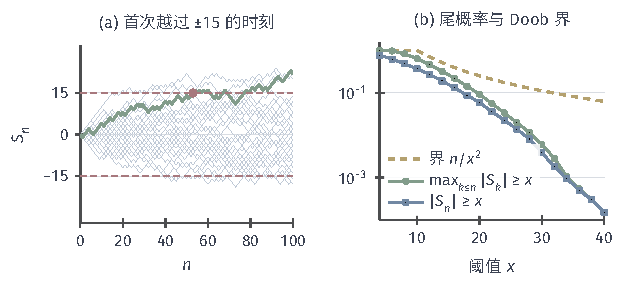
\includegraphics[width=106mm]{figures/03-optimization-evolution-and-signals/02-processes-and-trajectory-evolution/tikz/dtsp-doob-maximal/figure.pdf}
  \caption{Doob最大不等式。$S_n$为公平$\pm1$游走，$n=100$。(a)$40$条模拟路径，绿色路径在红点处首次达到$|S_k|\geq15$，在那里停止即把最大值事件化为停止事件；(b)$20000$次模拟得到的$\mathbb P(\max_{k\leq n}|S_k|\geq x)$与$\mathbb P(|S_n|\geq x)$，黄色虚线为界$\min\{1,n/x^2\}$。}
  \label{fig:dtsp-doob-maximal}
\end{figure}

\paragraph{非负超鞅的越界：Ville不等式}
同一想法用于非负超鞅，还能把有限时段推广到全部时刻。这一形式将成为指数型界的统一出口。

\begin{theorem}[Ville不等式]
  \label{thm:dtsp-ville}
  设$(L_n)_{n\geq0}$是非负超鞅，$x>0$。则
  \[
    \mathbb P\Bigl(\sup_{n\geq0}L_n\geq x\Bigr)\leq\frac{\mathbb EL_0}{x}.
  \]
\end{theorem}

\begin{proof}
固定$0<x'<x$，令$\tau=\inf\{n:L_n\geq x'\}$。由超鞅的有界可选抽样，$\mathbb EL_{\tau\wedge n}\leq\mathbb EL_0$；由非负性，$L_{\tau\wedge n}\geq x'\,\mathbb I\{\tau\leq n\}$。所以$x'\,\mathbb P(\tau\leq n)\leq\mathbb EL_0$，令$n\to\infty$得$\mathbb P(\tau<\infty)\leq\mathbb EL_0/x'$。事件$\{\sup_nL_n\geq x\}$包含于$\{\tau<\infty\}$，因为上确界达到$x$意味着某个时刻超过$x'$。再令$x'\uparrow x$即得结论。引入$x'$是为了处理上确界只被逼近、不在任何时刻取到的情形。
\end{proof}

这条不等式在后文统称为\term{Ville不等式}（Ville's inequality）。若取$\mathbb EL_0\leq1$和$x=1/\delta$，它说非负超鞅在整个无穷时段中曾经达到$1/\delta$的概率至多$\delta$。下面的指数型界都按同一模式构造：先找一个以累计误差为指数的非负超鞅，再用Ville不等式读出概率。

\paragraph{有界增量：Azuma--Hoeffding不等式}
第一个指数界只假设每步增量落在已知长度的区间里。它需要一个关于单个变量的引理：均值为零、取值区间长度不超过$c$的变量，其指数矩不超过同方差尺度的高斯变量。

\begin{lemma}[条件Hoeffding引理]
  \label{lem:dtsp-conditional-hoeffding}
  设$\mathcal G$是子$\sigma$代数，$D$可积且$\mathbb E[D\mid\mathcal G]=0$。若存在对$\mathcal G$可测的$a\leq b$使$a\leq D\leq b$几乎必然，且$b-a\leq c$，$c$为常数，则对所有$\gamma\in\mathbb R$，
  \[
    \mathbb E[e^{\gamma D}\mid\mathcal G]\leq\exp\Bigl(\frac{\gamma^2c^2}{8}\Bigr)\qquad\text{几乎必然}.
  \]
\end{lemma}

\begin{proof}
在$\{a=b\}$上，$D=a$且条件均值为零，故$D=0$，结论平凡。以下在$\{a<b\}$上论证。指数函数是凸的，对$a\leq x\leq b$它位于连接两端点的弦下方：
\[
  e^{\gamma x}\leq\frac{b-x}{b-a}e^{\gamma a}+\frac{x-a}{b-a}e^{\gamma b}.
\]
代入$x=D$并对$\mathcal G$取条件期望；$a,b$对$\mathcal G$可测可以提出，$\mathbb E[D\mid\mathcal G]=0$，得到$\mathbb E[e^{\gamma D}\mid\mathcal G]\leq(be^{\gamma a}-ae^{\gamma b})/(b-a)$。记$\theta=-a/(b-a)\in[0,1]$、$s=\gamma(b-a)$，右侧的对数为$\psi(s)=\log\bigl[(1-\theta)e^{-\theta s}+\theta e^{(1-\theta)s}\bigr]$。直接求导可得$\psi(0)=\psi'(0)=0$，且$\psi''(s)=r(1-r)\leq1/4$，其中$r=\theta e^s/(1-\theta+\theta e^s)\in[0,1]$。由Taylor公式的积分余项，$\psi(s)\leq s^2/8\leq\gamma^2c^2/8$。
\end{proof}

\begin{theorem}[Azuma--Hoeffding不等式]
  \label{thm:dtsp-azuma}
  设$(M_n)$是鞅，$M_0=0$，鞅差满足$a_k\leq D_k\leq b_k$，其中$a_k,b_k$对$\mathcal F_{k-1}$可测且$b_k-a_k\leq c_k$，$c_k$为常数。记$C_n=\sum_{k\leq n}c_k^2>0$。则对$x>0$，
  \begin{equation}
    \mathbb P\Bigl(\max_{k\leq n}M_k\geq x\Bigr)\leq\exp\Bigl(-\frac{2x^2}{C_n}\Bigr).
    \label{eq:dtsp-azuma}
  \end{equation}
\end{theorem}

\begin{proof}
固定$\gamma>0$，令$L_k=\exp\bigl(\gamma M_k-\gamma^2\sum_{j\leq k}c_j^2/8\bigr)$。由引理~\ref{lem:dtsp-conditional-hoeffding}，$\mathbb E[L_k\mid\mathcal F_{k-1}]=L_{k-1}\mathbb E[e^{\gamma D_k}\mid\mathcal F_{k-1}]e^{-\gamma^2c_k^2/8}\leq L_{k-1}$，所以$(L_k)$是非负超鞅，$L_0=1$。对$k\leq n$有$\sum_{j\leq k}c_j^2\leq C_n$，因此在事件$\{\max_{k\leq n}M_k\geq x\}$上$\max_{k\leq n}L_k\geq\exp(\gamma x-\gamma^2C_n/8)$。Ville不等式给出
\[
  \mathbb P\Bigl(\max_{k\leq n}M_k\geq x\Bigr)\leq\exp\Bigl(-\gamma x+\frac{\gamma^2C_n}{8}\Bigr),
\]
取$\gamma=4x/C_n$即得式~\eqref{eq:dtsp-azuma}。
\end{proof}

证明没有用到鞅差之间的独立性，只用到“给定过去后均值为零、范围受控”。对独立有界变量，它退化为Hoeffding不等式。代价是它按每一步可能的最坏范围计费：只要增量可能取到$\pm1$，就按方差$1$的尺度算，哪怕这件事极少发生。

\paragraph{条件方差：Freedman不等式}
考虑一个稀疏下注的例子：每一步以$0.95$的概率不下注，以各$0.025$的概率赢或输$1$，共$n=1000$步。增量范围是$[-1,1]$，Azuma界为$\exp(-x^2/2000)$；但每步条件方差只有$0.05$，实际的累计方差只有$50$，远小于范围给出的$1000$。图~\ref{fig:dtsp-azuma-freedman}显示$x=30$时精确尾概率约为$1.8\times10^{-5}$，Azuma界却是$0.64$，几乎没有信息。要利用小的条件方差，需要把第~\ref{sec:dtsp-quadratic-variation}节的可预测二次变差放进指数超鞅。

\begin{figure}[htbp]
  \centering
  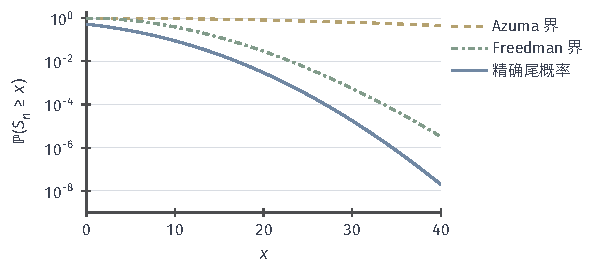
\includegraphics[width=100mm]{figures/03-optimization-evolution-and-signals/02-processes-and-trajectory-evolution/tikz/dtsp-azuma-freedman/figure.pdf}
  \caption{稀疏下注的尾概率与两种界（精确计算）。每步增量以概率$0.025$取$+1$、以$0.025$取$-1$、以$0.95$取$0$，$n=1000$。蓝线为由卷积精确算出的$\mathbb P(S_n\geq x)$；黄色虚线为Azuma界$\exp(-x^2/2n)$；绿色点划线为Freedman界$\exp\{-x^2/[2(v+x/3)]\}$，$v=50$为累计条件方差。纵轴为对数刻度。}
  \label{fig:dtsp-azuma-freedman}
\end{figure}

\begin{theorem}[Freedman不等式]
  \label{thm:dtsp-freedman}
  设$(D_k)$是鞅差，$|D_k|\leq b$几乎必然，$b>0$。记$S_n=\sum_{k\leq n}D_k$，$V_n=\langle S\rangle_n=\sum_{k\leq n}\mathbb E[D_k^2\mid\mathcal F_{k-1}]$。则对任意$x,v>0$，
  \begin{equation}
    \mathbb P\bigl(\exists n\geq1:\ S_n\geq x,\ V_n\leq v\bigr)\leq\exp\Bigl(-\frac{x^2}{2(v+bx/3)}\Bigr).
    \label{eq:dtsp-freedman}
  \end{equation}
\end{theorem}

\begin{proof}
先证一个标量不等式：对$0<\gamma<3/b$和$|u|\leq b$，
\[
  e^{\gamma u}\leq1+\gamma u+\frac{\gamma^2u^2}{2(1-\gamma b/3)}.
\]
展开指数级数，$k\geq2$项满足$(\gamma u)^k/k!\leq\frac{(\gamma u)^2}{2}(\gamma b/3)^{k-2}$，因为$k!\geq2\cdot3^{k-2}$；对$k\geq2$求和是一个几何级数。代入$u=D_k$并取条件期望，一次项消失，再用$1+t\leq e^t$：
\[
  \mathbb E[e^{\gamma D_k}\mid\mathcal F_{k-1}]\leq\exp\bigl(\phi(\gamma)\,\mathbb E[D_k^2\mid\mathcal F_{k-1}]\bigr),\qquad
  \phi(\gamma)=\frac{\gamma^2}{2(1-\gamma b/3)}.
\]
因此$L_n=\exp(\gamma S_n-\phi(\gamma)V_n)$是非负超鞅，$L_0=1$。在$\{S_n\geq x,V_n\leq v\}$上$L_n\geq\exp(\gamma x-\phi(\gamma)v)$，于是由Ville不等式，左侧概率不超过$\exp(-\gamma x+\phi(\gamma)v)$。取$\gamma=x/(v+bx/3)$，它落在$(0,3/b)$内，且$1-\gamma b/3=v/(v+bx/3)$，代入后指数恰为$-x^2/[2(v+bx/3)]$。
\end{proof}

Freedman界的分母有两项。小偏差时$v$主导，界像方差为$v$的高斯尾；大偏差时$bx/3$主导，界退化为指数尾，反映单步增量最多为$b$。对独立有界变量，$V_n$是确定数，式~\eqref{eq:dtsp-freedman}在固定$n$处给出Bernstein型不等式；对鞅，$V_n$随路径变化，事件中“$V_n\leq v$”这一项把界限定在实际波动不大的路径上。回到第~\ref{sec:dtsp-quadratic-variation}节领先时加注的赌徒：长期落后的路径$V_n$接近$n/4$，界随之收紧。

\paragraph{查看时刻与同时成立的保证}
上面三个界的时间量词不同，使用时要和查看方式对应。只在预先固定的时刻$n$查看，固定时刻的界就够了。若最多查看$T$次，可以给第$t$次分配失败概率$\delta_t$，只要$\sum_t\delta_t\leq\delta$，并合界就保证总失败概率不超过$\delta$。若查看时刻由数据决定，例如“第一次看起来足够好时停止”，就需要对所有时刻同时成立的保证：若$\mathbb P(\bigcup_{n\geq1}E_n)\leq\delta$，则对任何几乎必然有限的停时$\tau$都有$\mathbb P(E_\tau)\leq\delta$。Doob与Azuma界的最大值形式、Ville不等式和Freedman界都属于这一类，它们来自非负超鞅，而不是把固定时刻界中的$n$换成随机时刻。

\paragraph{可预测设计下的自归一化界}
在许多序贯问题中，每一步先根据历史选一个查询方向，再观测带噪响应。设参数$\bm\theta^\star\in\mathbb R^d$未知，第$k$步选择特征$\bm x_k\in\mathbb R^d$，观测
\begin{equation}
  y_k=\bm x_k^{\top}\bm\theta^\star+\varepsilon_k.
  \label{eq:stoch-adaptive-linear-observation}
\end{equation}
特征可以依赖此前的全部结果，但必须在$\varepsilon_k$揭晓之前确定，即$(\bm x_k)$可预测；噪声$\varepsilon_k$对$\mathcal F_k$可测。下面关心的累计量是噪声沿所选方向的加权和$\bm S_n=\sum_{k\leq n}\bm x_k\varepsilon_k$，它是历史适应的随机累计量。

先给噪声一个条件尾部假设。若存在$\sigma>0$，使对每个$k$和每个$\gamma\in\mathbb R$，
\begin{equation}
  \mathbb E[e^{\gamma\varepsilon_k}\mid\mathcal F_{k-1}]\leq\exp\Bigl(\frac{\gamma^2\sigma^2}{2}\Bigr)\qquad\text{几乎必然},
  \label{eq:dtsp-conditional-subgaussian}
\end{equation}
称$(\varepsilon_k)$为参数$\sigma^2$的\term{条件次高斯鞅差}（conditionally sub-Gaussian martingale difference）。名称中的“鞅差”是这一条件的推论：由$e^{\gamma u}\geq1+\gamma u$得$\gamma\,\mathbb E[\varepsilon_k\mid\mathcal F_{k-1}]\leq e^{\gamma^2\sigma^2/2}-1$，分别令$\gamma\downarrow0$与$\gamma\uparrow0$，得到条件均值为零。有界噪声由引理~\ref{lem:dtsp-conditional-hoeffding}满足此条件，高斯噪声取其方差即可。

特征可预测时，$\bm S_n$的每个坐标都是定理~\ref{thm:dtsp-martingale-transform}意义下的鞅变换。自然的误差尺度不是欧氏范数：某个方向被反复查询后，累计噪声在该方向上的规模也随之增长，应当按“该方向积累了多少信息”来归一化。取事先固定的$\lambda>0$，令
\[
  \bm V_n=\lambda\bm I+\sum_{k=1}^n\bm x_k\bm x_k^{\top},\qquad
  \lVert\bm S_n\rVert_{\bm V_n^{-1}}=\sqrt{\bm S_n^{\top}\bm V_n^{-1}\bm S_n}.
\]
$\bm V_n$在常被查询的方向上大，逆矩阵就在这些方向上小。用随机设计矩阵本身来度量累计噪声的做法称为\term{自归一化}（self-normalized）。

\begin{theorem}[向量自归一化界]
  \label{thm:dtsp-self-normalized}
  设$(\bm x_k)$可预测，$(\varepsilon_k)$满足式~\eqref{eq:dtsp-conditional-subgaussian}。则对任意$\delta\in(0,1)$，以至少$1-\delta$的概率，对所有$n\geq0$同时有
  \begin{equation}
    \lVert\bm S_n\rVert_{\bm V_n^{-1}}^2\leq2\sigma^2\log\Bigl(\frac{\det(\bm V_n)^{1/2}\det(\lambda\bm I)^{-1/2}}{\delta}\Bigr).
    \label{eq:stoch-vector-self-normalized-bound}
  \end{equation}
\end{theorem}

\begin{proof}
第一步，固定方向。对固定的$\bm u\in\mathbb R^d$，$\gamma_k=\bm u^{\top}\bm x_k$对$\mathcal F_{k-1}$可测。式~\eqref{eq:dtsp-conditional-subgaussian}对确定的$\gamma$成立；对只取有限个有理值的$\mathcal F_{k-1}$可测$\gamma_k$，在各取值事件上分别使用它即可；一般的$\gamma_k$用这类简单函数逐点逼近，再对每个$A\in\mathcal F_{k-1}$用Fatou引理，得到
\[
  \mathbb E\bigl[e^{\gamma_k\varepsilon_k-\sigma^2\gamma_k^2/2}\bigm|\mathcal F_{k-1}\bigr]\leq1.
\]
逐步相乘可知$L_n(\bm u)=\exp\bigl(\bm u^{\top}\bm S_n-\frac{\sigma^2}{2}\bm u^{\top}(\bm V_n-\lambda\bm I)\bm u\bigr)$是非负超鞅，$L_0(\bm u)=1$。

第二步，对所有方向取平均。固定方向只能控制一个投影；为同时控制所有方向，取与数据独立的高斯权重$\bm U\sim\mathcal N(\bm 0,(\sigma^2\lambda)^{-1}\bm I)$，定义$\overline L_n=\mathbb E_{\bm U}[L_n(\bm U)]$。非负性允许交换条件期望与对$\bm U$的积分（Tonelli定理），所以$\overline L_n$仍是非负超鞅，$\overline L_0=1$。把高斯密度与指数中的二次型合并，指数变为$\bm u^{\top}\bm S_n-\frac{\sigma^2}{2}\bm u^{\top}\bm V_n\bm u$，配方后积分得到
\[
  \overline L_n=\Bigl(\frac{\det(\lambda\bm I)}{\det(\bm V_n)}\Bigr)^{1/2}\exp\Bigl(\frac{\lVert\bm S_n\rVert_{\bm V_n^{-1}}^2}{2\sigma^2}\Bigr).
\]
行列式比来自两个高斯积分的归一化常数，指数项来自配方后中心的移动。

第三步，读出概率。由Ville不等式，$\mathbb P(\sup_n\overline L_n\geq1/\delta)\leq\delta$。在补事件上对所有$n$都有$\overline L_n<1/\delta$，取对数整理即为式~\eqref{eq:stoch-vector-self-normalized-bound}。
\end{proof}

各项假设各有分工。条件次高斯性构造每一步的指数超鞅；特征可预测性让$\bm x_k$在条件期望中被当作已知；$\lambda>0$使高斯混合与逆矩阵从$n=0$起就有定义。行列式$\det\bm V_n$记录各方向信息的共同增长：重复查询同一方向与首次查询新方向提供的信息不同，所以不能把它简单换成查询次数。这里只建立历史适应累计量的偏差界；据此为$\bm\theta^\star$构造置信集合、分析序贯决策的统计性质，属于统计推断与决策部分的任务。还应注意，这里的“自归一化”与第~\ref{sec:dtsp-importance}节自归一化重要性抽样中的“权重之和作分母”不是同一个对象。

\subsection{鞅的极限与期望保持}
\label{sec:dtsp-martingale-limits}

\paragraph{上穿次数}
现在让时间趋于无穷。一条实值路径没有极限，当且仅当它的下极限严格小于上极限；这时可以找到两个有理数$a<b$夹在中间，路径无穷多次从$a$以下走到$b$以上。把一次“从$\leq a$出发、到达$\geq b$”称为对区间$[a,b]$的一次\term{上穿}（upcrossing），记前$n$步完成的上穿次数为$U_n[a,b]$。图~\ref{fig:dtsp-upcrossings}(a)中，公平游走在$300$步内对$[-2,4]$完成了$3$次上穿。要证明收敛，只需证明对每一对有理数$a<b$，总上穿次数几乎必然有限。

上穿次数可以用一个下注策略来数：价格跌到$a$以下就买入，涨到$b$以上就卖出。每完成一次上穿至少赚$b-a$，最后一笔若尚未卖出，亏损不超过$(X_n-a)^-$。而这个策略只依据过去的价格决定是否持有，是可预测的；在超鞅（不利的市场）中，任何可预测的非负有界策略期望收益都不为正。两者对照，就得到上穿次数期望的界。

\begin{theorem}[Doob上穿不等式]
  \label{thm:dtsp-upcrossing}
  设$(X_n)$是超鞅，$a<b$。则$(b-a)\,\mathbb EU_n[a,b]\leq\mathbb E(X_n-a)^-$。
\end{theorem}

\begin{proof}
令$H_0=0$，并对$k\geq1$定义持有指示$H_k=\mathbb I\{H_{k-1}=1,X_{k-1}<b\}+\mathbb I\{H_{k-1}=0,X_{k-1}\leq a\}$：未持有时一旦价格$\leq a$就买入，持有时直到价格$\geq b$才卖出。$H_k$只用到$X_0,\ldots,X_{k-1}$，可预测，且取值于$\{0,1\}$。把收益$(H\cdot X)_n$按持有区间分组：每个完整的持有区间对应一次上穿，收益至少$b-a$；最后一个未结束的区间从某个$\leq a$的价格买入，收益至少$X_n-a\geq-(X_n-a)^-$。因此$(H\cdot X)_n\geq(b-a)U_n[a,b]-(X_n-a)^-$。由定理~\ref{thm:dtsp-martingale-transform}，$H\cdot X$是超鞅，$\mathbb E(H\cdot X)_n\leq0$，整理即得。
\end{proof}

\paragraph{几乎必然收敛}
上穿不等式把“无穷振荡”与“期望有界”对立起来。

\begin{theorem}[超鞅收敛定理]
  \label{thm:dtsp-supermartingale-convergence}
  设$(X_n)$是超鞅，且$\sup_n\mathbb EX_n^-<\infty$。则$X_n$几乎必然收敛到一个可积随机变量$X_\infty$。特别地，非负超鞅几乎必然收敛；满足$\sup_n\mathbb E|M_n|<\infty$的鞅几乎必然收敛。
\end{theorem}

\begin{proof}
对有理数$a<b$，$\mathbb E(X_n-a)^-\leq|a|+\mathbb EX_n^-$有与$n$无关的上界。由单调收敛，$\mathbb EU_\infty[a,b]=\lim_n\mathbb EU_n[a,b]<\infty$，所以$U_\infty[a,b]<\infty$几乎必然。可数多对有理数的例外集合之并仍是零概率事件，在其补集上$\liminf X_n=\limsup X_n$，即$X_n$在$[-\infty,\infty]$中有极限$X_\infty$。又$\mathbb E|X_n|=\mathbb EX_n+2\mathbb EX_n^-\leq\mathbb EX_0+2\sup_k\mathbb EX_k^-$，由Fatou引理$\mathbb E|X_\infty|\leq\liminf_n\mathbb E|X_n|<\infty$，所以极限几乎必然有限且可积。非负超鞅满足$X_n^-=0$；对鞅，把定理用于$M_n$本身即可。
\end{proof}

图~\ref{fig:dtsp-upcrossings}(b)是一个有界鞅的例子。坛子里起初有红、蓝球各一个，每次随机摸一个球，放回并再加入一个同色球。记摸了$n$次后红球比例为$F_n=R_n/(n+2)$，则$\mathbb E[F_{n+1}\mid\mathcal F_n]=(R_n+F_n)/(n+3)=F_n$，所以$(F_n)$是取值于$[0,1]$的鞅，必然几乎处处收敛。图中十二次实验的比例很快稳定下来，但稳定在不同的位置：极限是随机的，实际上服从$[0,1]$上的均匀分布。鞅收敛定理保证每条路径都会停下来，却不规定停在哪里。

\begin{figure}[htbp]
  \centering
  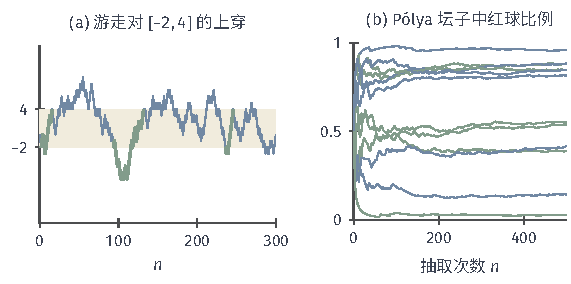
\includegraphics[width=97mm]{figures/03-optimization-evolution-and-signals/02-processes-and-trajectory-evolution/tikz/dtsp-upcrossings/figure.pdf}
  \caption{上穿与鞅收敛。(a)公平$\pm1$游走的一条$300$步模拟路径，绿色粗线标出对区间$[-2,4]$（黄色带）完成的上穿；游走不收敛，上穿次数随时间无限增长。(b)Pólya坛子（初始红、蓝各一球，每次加入一个与摸出球同色的球）中红球比例的$12$次模拟，比例是有界鞅，各自收敛到不同的随机极限。}
  \label{fig:dtsp-upcrossings}
\end{figure}

路径收敛并不意味着期望收敛。在“加倍或清零”的乘积鞅$M_n=\prod_{k\leq n}Y_k$中（$Y_k$等概率取$0,2$），只要出现一次$0$，此后就恒为零，所以$M_n\to0$几乎必然；但$\mathbb EM_n=1$对所有$n$成立。概率越来越小的路径上保留着越来越大的值，这部分期望在极限中消失了，与加倍下注中“跑到无穷远”的负质量是同一现象。

\paragraph{一致可积与平均收敛}
要让极限保持期望，就要排除上面这种期望集中在越来越小事件上的情形，这正是一致可积的含义。

\begin{theorem}[一致可积鞅]
  \label{thm:dtsp-ui-martingale}
  对鞅$(M_n)$，以下三条等价：(1)$(M_n)$一致可积；(2)$M_n$几乎必然且在$L^1$中收敛到某个$M_\infty$；(3)存在可积随机变量$Z$使$M_n=\mathbb E[Z\mid\mathcal F_n]$对所有$n$成立。此时$M_n=\mathbb E[M_\infty\mid\mathcal F_n]$，且$M_\infty=\mathbb E[Z\mid\mathcal F_\infty]$，其中$\mathcal F_\infty=\sigma(\bigcup_n\mathcal F_n)$。
\end{theorem}

\begin{proof}
(1)$\Rightarrow$(2)：一致可积推出$\sup_n\mathbb E|M_n|<\infty$，由定理~\ref{thm:dtsp-supermartingale-convergence}几乎必然收敛；几乎必然收敛加一致可积推出$L^1$收敛。(2)$\Rightarrow$(3)：对$A\in\mathcal F_n$与$m\geq n$，$\mathbb E[M_m\mathbb I_A]=\mathbb E[M_n\mathbb I_A]$；令$m\to\infty$，$L^1$收敛允许取极限，得$\mathbb E[M_\infty\mathbb I_A]=\mathbb E[M_n\mathbb I_A]$，所以$M_n=\mathbb E[M_\infty\mid\mathcal F_n]$，取$Z=M_\infty$。(3)$\Rightarrow$(1)：由条件Jensen不等式$|M_n|\leq\mathbb E[|Z|\mid\mathcal F_n]$，而$\{|M_n|>K\}\in\mathcal F_n$，故
\[
  \mathbb E[|M_n|;|M_n|>K]\leq\mathbb E[|Z|;|M_n|>K],\qquad\mathbb P(|M_n|>K)\leq\frac{\mathbb E|Z|}{K}.
\]
单个可积变量$|Z|$在小概率事件上的积分一致地小：对任意$\varepsilon>0$存在$\eta>0$，使$\mathbb P(A)<\eta$时$\mathbb E[|Z|;A]<\varepsilon$。取$K>\mathbb E|Z|/\eta$，便对所有$n$有$\mathbb E[|M_n|;|M_n|>K]<\varepsilon$。最后一句：$M_\infty$对$\mathcal F_\infty$可测，且对$A\in\bigcup_n\mathcal F_n$有$\mathbb E[M_\infty\mathbb I_A]=\mathbb E[Z\mathbb I_A]$；满足此等式的$A$构成$\lambda$系，而$\bigcup_n\mathcal F_n$是$\pi$系，由$\pi$-$\lambda$定理推广到$\mathcal F_\infty$。
\end{proof}

条件(3)说，一致可积鞅恰好是“对同一个终极量的逐步预测”。Pólya坛子比例有界，因而一致可积，$\mathbb EF_\infty=\mathbb EF_0=1/2$；乘积鞅$\prod Y_k$不一致可积，不能写成某个固定变量的条件期望。这也解释了定理~\ref{thm:dtsp-optional-stopping}的第三个条件：停止过程一致可积时，它是对$M_\tau$的逐步预测，期望得以保持。

\paragraph{平方可积鞅}
若有二阶矩的统一上界，结论更强也更好用，因为正交增量给出了误差的精确表达。

\begin{theorem}[$L^2$鞅收敛]
  \label{thm:dtsp-l2-martingale}
  设$(M_n)$是鞅且$\sup_n\mathbb EM_n^2<\infty$。则$M_n$几乎必然且在$L^2$中收敛到$M_\infty$，并且
  \[
    \mathbb E(M_\infty-M_n)^2=\sum_{k>n}\mathbb ED_k^2.
  \]
\end{theorem}

\begin{proof}
由式~\eqref{eq:dtsp-orthogonal-increments}，$\sum_k\mathbb ED_k^2=\sup_n\mathbb EM_n^2-\mathbb EM_0^2<\infty$。对$m>n$，正交性给出$\mathbb E(M_m-M_n)^2=\sum_{k=n+1}^m\mathbb ED_k^2$，它随$n\to\infty$趋于零，所以$(M_n)$在$L^2$中是Cauchy列，收敛到某个$M_\infty$。另一方面$\sup_n\mathbb E|M_n|\leq\sup_n(\mathbb EM_n^2)^{1/2}<\infty$，由定理~\ref{thm:dtsp-supermartingale-convergence}几乎必然收敛；两个极限几乎必然相等。令$m\to\infty$即得误差公式。
\end{proof}

几种结论所需的条件不同，不能把同一组充分条件套给所有收敛方式：$L^1$有界保证几乎必然收敛但不保证期望保持；一致可积再保证$L^1$收敛与条件期望表示；$L^2$有界保证$L^2$收敛，并把尾部误差写成剩余增量方差之和。

\subsection{加权噪声与几乎超鞅}
\label{sec:dtsp-weighted-noise}

本小节把上面的收敛定理改写成两条可以直接用于带噪递推的判据。第一条处理随时间缩小权重的累计噪声，第二条处理“平均下降、但有小扰动”的非负量。

\paragraph{加权鞅差和的收敛}
在随机递推中，第$k$步的噪声$D_k$乘以步长$\alpha_k$后才进入状态。直观上，若$\sum_k\alpha_k^2$乘上条件方差后有限，累计噪声的总方差就有限，加权和应当停下来。下面的定理允许权重和条件方差都依赖历史，只要求它们沿每条路径的累计有限。

\begin{theorem}[加权鞅差和的收敛]
  \label{thm:dtsp-weighted-martingale-sum}
  设$(D_k)$是平方可积鞅差，$(\alpha_k)$是可预测实值过程。若
  \[
    \sum_{k\geq1}\alpha_k^2\,\mathbb E[D_k^2\mid\mathcal F_{k-1}]<\infty\qquad\text{几乎必然},
  \]
  则$\sum_{k\geq1}\alpha_kD_k$几乎必然收敛。特别地，若$\alpha_k$是确定数，$\sum_k\alpha_k^2<\infty$，且$\mathbb E[D_k^2\mid\mathcal F_{k-1}]\leq\sigma^2$，则结论成立，并且部分和在$L^2$中也收敛。
\end{theorem}

\begin{proof}
记$N_n=\sum_{k\leq n}\alpha_kD_k$，$Q_n=\sum_{k\leq n}\alpha_k^2\mathbb E[D_k^2\mid\mathcal F_{k-1}]$。$Q_{n+1}$对$\mathcal F_n$可测，所以对$c>0$，$\tau_c=\inf\{n\geq0:Q_{n+1}>c\}$是停时。考虑停止过程$N_{\tau_c\wedge n}=\sum_{k\leq n}\mathbb I\{\tau_c\geq k\}\alpha_kD_k$。在$\{\tau_c\geq k\}$上$Q_k\leq c$，于是
\[
  \mathbb E\bigl[\mathbb I\{\tau_c\geq k\}\alpha_k^2D_k^2\bigr]=\mathbb E\bigl[\mathbb I\{\tau_c\geq k\}\alpha_k^2\,\mathbb E[D_k^2\mid\mathcal F_{k-1}]\bigr]\leq c,
\]
每个增量平方可积，停止过程是鞅，且由正交性$\mathbb EN_{\tau_c\wedge n}^2=\mathbb EQ_{\tau_c\wedge n}\leq c$。定理~\ref{thm:dtsp-l2-martingale}给出$N_{\tau_c\wedge n}$几乎必然收敛。在事件$\{\tau_c=\infty\}$上$N_n=N_{\tau_c\wedge n}$，所以$N_n$收敛。最后，$\{Q_\infty<\infty\}=\bigcup_{c\in\mathbb N}\{\tau_c=\infty\}$的概率为一。确定权重的情形中$Q_\infty\leq\sigma^2\sum\alpha_k^2$，$N_n$本身$L^2$有界。
\end{proof}

例如独立公平符号$\xi_k$的随机调和级数$\sum_k\xi_k/k$几乎必然收敛，因为$\sum_k k^{-2}<\infty$；而$\sum_k\xi_k/\sqrt k$的权重平方和发散，定理不适用；由独立随机级数的三级数判别可知它几乎必然不收敛。

定理还给出鞅差的大数定律。若$\mathbb E[D_k^2\mid\mathcal F_{k-1}]\leq\sigma^2$，取$\alpha_k=1/k$，则$\sum_kD_k/k$收敛。确定性的\term{Kronecker引理}（Kronecker lemma）说：若$0<b_k\uparrow\infty$且$\sum_kx_k/b_k$收敛，则$b_n^{-1}\sum_{k\leq n}x_k\to0$。证明只需分部求和：记$r_k=\sum_{j>k}x_j/b_j\to0$，则$\sum_{k\leq n}x_k=b_1r_0-b_nr_n+\sum_{k=1}^{n-1}(b_{k+1}-b_k)r_k$，除以$b_n$后最后一项是$r_k$的加权平均，权重之和不超过一，而$r_k\to0$，所以它也趋于零。取$b_k=k$便得到
\begin{equation}
  \frac1n\sum_{k=1}^nD_k\longrightarrow0\qquad\text{几乎必然}.
  \label{eq:dtsp-martingale-lln}
\end{equation}
这是独立同分布强大数律在鞅差上的推广：增量不必独立，只需给定过去后均值为零且条件方差有统一上界。

\paragraph{几乎超鞅}
随机递推的稳定性分析常落到一个非负“能量”上，例如误差平方。每一步它平均下降一点，却可能被噪声或偏差略微抬高。若抬高的部分可求和，能量就应当收敛，而且累计下降量有限。下面的结论把这一直觉写成定理，它在第~\ref{sec:dtsp-stochastic-approximation}节反复使用。

\begin{theorem}[几乎超鞅收敛]
  \label{thm:dtsp-almost-supermartingale}
  设$Z_n,A_n$是非负、可积、适应的过程，$\beta_n,b_n\geq0$是确定数，满足$\sum_n\beta_n<\infty$、$\sum_nb_n<\infty$，且
  \begin{equation}
    \mathbb E[Z_{n+1}\mid\mathcal F_n]\leq(1+\beta_n)Z_n+b_n-A_n\qquad\text{几乎必然}.
    \label{eq:dtsp-almost-supermartingale}
  \end{equation}
  则$Z_n$几乎必然收敛到有限随机变量，并且$\sum_nA_n<\infty$几乎必然。
\end{theorem}

\begin{proof}
先消去乘性扰动。令$\pi_n=\prod_{k<n}(1+\beta_k)$，它单调上升并收敛到有限的$\pi_\infty$，因为$\log\pi_n\leq\sum_k\beta_k$。记$Z_n'=Z_n/\pi_n$、$b_n'=b_n/\pi_{n+1}$、$A_n'=A_n/\pi_{n+1}$，把式~\eqref{eq:dtsp-almost-supermartingale}除以$\pi_{n+1}$得$\mathbb E[Z_{n+1}'\mid\mathcal F_n]\leq Z_n'+b_n'-A_n'$。再吸收加性扰动：令$U_n=Z_n'+\sum_{k\geq n}b_k'$，则$\mathbb E[U_{n+1}\mid\mathcal F_n]\leq U_n-A_n'\leq U_n$，所以$(U_n)$是非负超鞅，由定理~\ref{thm:dtsp-supermartingale-convergence}几乎必然收敛到有限值。尾和$\sum_{k\geq n}b_k'\to0$，故$Z_n'$收敛，$Z_n=\pi_nZ_n'$也收敛。最后，对$\mathbb E[U_{k+1}]\leq\mathbb E[U_k]-\mathbb E[A_k']$从$0$到$n$求和得$\mathbb E\sum_{k\leq n}A_k'\leq\mathbb EU_0<\infty$，由单调收敛$\sum_kA_k'$几乎必然有限，而$A_k\leq\pi_\infty A_k'$。
\end{proof}

这个定理只给出“收敛”与“累计下降有限”两件事，并不直接说明极限是多少。确定极限还要把$\sum_nA_n<\infty$与问题结构结合起来，例如$A_n=\alpha_nZ_n$且$\sum\alpha_n=\infty$时，极限只能是零。当$\beta_n,b_n$是可预测的随机量、只在几乎必然意义下可求和时，结论仍然成立，证明需要像定理~\ref{thm:dtsp-weighted-martingale-sum}那样对随机和作局部化，这里不再展开。

\section{长期分布与时间平均}
\label{sec:dtsp-long-run}

现在回到第~\ref{sec:dtsp-visits}节留下的问题：链运行很久以后会怎样。这里有两个不同的问题。其一，某个很晚的时刻$n$，状态$X_n$服从什么分布，它是否趋向不变分布，速度多快？其二，沿一条长轨迹计算平均$\frac1n\sum_{k<n}f(X_k)$，它是否趋向某个常数，误差有多大？前者关心的是“很多次独立重复运行、在同一时刻拍快照”，后者关心的是“一次运行、沿时间累计”。周期链已经表明二者可以不同：快照分布永远振荡，时间平均却收敛。本节先用时间平移描述“统计规律不变”，再分别研究这两个问题。

\subsection{平稳性与时间平移}
\label{sec:dtsp-stationarity}

\paragraph{严格平稳}
不变分布描述的是单个时刻的分布不变。更强的要求是：把整个观察窗口向后平移，所有时刻的联合规律都不变。

\begin{definition}[平稳过程]
  \label{def:dtsp-stationary-process}
  过程$(X_n)_{n\geq0}$称为（严格）\term{平稳过程}（stationary process），若对任意正整数$m$、时刻$n_1,\ldots,n_m\geq0$和平移量$h\geq0$，
  \[
    (X_{n_1},\ldots,X_{n_m})\overset{\mathrm d}{=}(X_{n_1+h},\ldots,X_{n_m+h}).
  \]
\end{definition}

\begin{theorem}[从不变分布启动的链是平稳的]
  \label{thm:dtsp-stationary-chain}
  设$(X_n)$是以$P$为转移核的时间齐次Markov链，$X_0\sim\pi$且$\pi P=\pi$。则$(X_n)$是平稳过程。
\end{theorem}

\begin{proof}
只需检查连续窗口$(X_h,\ldots,X_{h+m})$的规律不依赖$h$，因为任意有限组时刻都是某个连续窗口的边缘。由Markov性质，这一窗口的联合规律是$\mu_h(\mathrm dx_0)P(x_0,\mathrm dx_1)\cdots P(x_{m-1},\mathrm dx_m)$，其中$\mu_h$是$X_h$的分布。而$\mu_h=\pi P^h=\pi$，所以联合规律与$h$无关。
\end{proof}

只知道某一时刻的边缘等于$\pi$并不够：上面的论证同时用到了核不变与Markov结构。例如图~\ref{fig:dtsp-ar1-path-bundle}中的递推若从$X_0\sim\mathcal N(0,1/0.36)$启动，每个$X_n$都服从同一个正态分布，而且整个过程平稳；两步之间的协方差为$\operatorname{Cov}(X_n,X_{n+k})=0.8^k/0.36$，只依赖间隔$k$。平稳并不意味着独立，相邻读数仍以$0.8$的系数相关。

\paragraph{二阶平稳}
若只计算均值和二阶误差，可以只要求均值不变、协方差只依赖时间差。具有有限二阶矩的实值过程若$\mathbb EX_n$与$n$无关、$\operatorname{Cov}(X_n,X_{n+k})$只依赖$k$，称为\term{二阶平稳}（second-order stationarity），也称弱平稳。严格平稳且二阶矩有限蕴含二阶平稳；反之不成立。取相互独立的序列，偶数时刻服从标准正态，奇数时刻等概率取$\pm1$：均值都是零，方差都是一，不同时刻的协方差都是零，所以二阶平稳；但一维边缘随奇偶改变，不是严格平稳。联合高斯过程的有限维分布由均值与协方差完全确定，对它们二者等价。二阶平稳过程的频谱表示与线性滤波属于信号与状态估计部分，这里不展开。

\paragraph{平稳过程与平稳增量}
公平游走$S_n$的方差为$n$，随时间增长，不是平稳过程；但它的增量$\xi_n$独立同分布，因而增量过程平稳。类似的区分对连续时间的Brownian运动同样重要。同一个公平游走因此同时是Markov链、鞅，且具有平稳增量，而它本身不平稳：这几种结构回答不同的问题，并不互斥。

\subsection{Markov链的分布收敛}
\label{sec:dtsp-distribution-convergence}

\paragraph{用总变差比较分布}
要说$X_n$的分布“接近”$\pi$，先要有一个比较分布的尺度。最直接的尺度是：有没有某个事件，两个分布给它的概率差得很多。对同一可测空间上的概率测度$\mu,\nu$，定义
\[
  \lVert\mu-\nu\rVert_{\mathrm{TV}}=\sup_{B\in\mathcal E}|\mu(B)-\nu(B)|,
\]
称为\term{总变差距离}（total variation distance）。可数状态时它等于$\frac12\sum_i|\mu_i-\nu_i|$：令$B^\ast=\{i:\mu_i>\nu_i\}$，两者总质量相等，故$\mu(B^\ast)-\nu(B^\ast)=\frac12\sum_i|\mu_i-\nu_i|$；对任意$B$，$\mu(B)-\nu(B)\leq\mu(B\cap B^\ast)-\nu(B\cap B^\ast)\leq\mu(B^\ast)-\nu(B^\ast)$，另一侧对称。总变差为$0.01$意味着没有任何事件的概率被改变超过$0.01$。概率分布之间更一般的距离与几何留到概率分布部分，本章只用这一种。

\paragraph{耦合：让两条链相遇}
怎样证明从$x$出发的链“忘记”了起点？一个形象的办法是让两个人同时在转移图上随机行走，一个从$x$出发，另一个从$\pi$中随机选起点。两人各自独立行走，一旦站在同一个状态，就从此手拉手一起走。相遇以后两人的位置永远相同；而第二个人始终服从$\pi$，因为$\pi$不变。于是第一个人在时刻$n$的分布与$\pi$的差别，不会超过“到时刻$n$两人还没相遇”的概率。

把这一想法写成不等式。若随机对$(X,Y)$满足$X\sim\mu$、$Y\sim\nu$，则对任意$B$，$\mu(B)-\nu(B)=\mathbb P(X\in B)-\mathbb P(Y\in B)\leq\mathbb P(X\in B,Y\notin B)\leq\mathbb P(X\neq Y)$，因此
\begin{equation}
  \lVert\mu-\nu\rVert_{\mathrm{TV}}\leq\mathbb P(X\neq Y).
  \label{eq:dtsp-coupling-inequality}
\end{equation}
上面的“手拉手”构造中，第二条链在相遇时刻（一个停时）之后改为跟随第一条链，由强Markov性质它仍是以$P$为转移核的链。若$T$是相遇时刻，便有$\lVert P^n(x,\cdot)-\pi\rVert_{\mathrm{TV}}\leq\mathbb P(T>n)$。剩下的问题是让相遇足够快，下面用一步一步的“最大重合”把它量化。

\paragraph{一步转移的收缩系数}
对转移核$Q$，定义\term{Dobrushin系数}（Dobrushin coefficient）
\[
  \delta(Q)=\sup_{x,x'}\lVert Q(x,\cdot)-Q(x',\cdot)\rVert_{\mathrm{TV}}.
\]
它度量“从两个最不相同的起点出发，走一步后的分布最多还差多少”。可数状态时，$\delta(Q)=1-\min_{x,x'}\sum_y\min\{Q(x,y),Q(x',y)\}$：每对行向量的公共部分越多，一步后越难分辨起点。

\begin{lemma}[总变差的收缩]
  \label{lem:dtsp-dobrushin}
  对可数状态上的概率分布$\mu,\nu$与转移核$Q$，$\lVert\mu Q-\nu Q\rVert_{\mathrm{TV}}\leq\delta(Q)\lVert\mu-\nu\rVert_{\mathrm{TV}}$。
\end{lemma}

\begin{proof}
记$t=\lVert\mu-\nu\rVert_{\mathrm{TV}}$，设$t>0$。差$\mu-\nu$的正部与负部总质量都是$t$，于是可写$\mu-\nu=t(\alpha-\beta)$，其中$\alpha,\beta$是概率分布。从而
\[
  \mu Q-\nu Q=t(\alpha Q-\beta Q)=t\sum_{x,x'}\alpha_x\beta_{x'}\bigl(Q(x,\cdot)-Q(x',\cdot)\bigr).
\]
可数状态上$\lVert\cdot\rVert_{\mathrm{TV}}$等于半个$\ell^1$范数，满足三角不等式，故右侧的总变差至多$t\sum_{x,x'}\alpha_x\beta_{x'}\delta(Q)=t\,\delta(Q)$。
\end{proof}

对两状态链~\eqref{eq:dtsp-two-state-matrix}，两行的公共部分为$\min(0.9,0.2)+\min(0.1,0.8)=0.3$，所以$\delta(\bm P)=0.7$，恰好是式~\eqref{eq:dtsp-two-state-power}中的衰减率。确定交替链的两行没有公共部分，$\delta=1$，而且对所有$n$都有$\delta(\bm P^n)=1$：它永远不收缩。周期正是使所有幂的行向量支撑错开的结构。

\paragraph{有限非周期链的几何收敛}
要让某个幂$\bm P^m$的任意两行都有公共部分，只需$\bm P^m$的每个元素都为正。非周期性恰好保证这一点。

\begin{lemma}[非周期链的正幂]
  \label{lem:dtsp-positive-power}
  有限、不可约、非周期的转移矩阵$\bm P$存在整数$m$，使$\bm P^m$的所有元素严格为正。
\end{lemma}

\begin{proof}
固定状态$i$，返回步数集$R_i$对加法封闭（先走一个回路再走另一个），且$\gcd R_i=1$。先证$R_i$包含所有足够大的整数。取有限个元素使其最大公约数为$1$，由Bezout等式存在整数系数把$1$写成它们的组合；把正系数项与负系数项分开，得到$A,B\in R_i\cup\{0\}$使$A-B=1$。若$B=0$则$1\in R_i$，结论平凡。否则对$n\geq B^2$，写$n=qB+r$，$0\leq r<B\leq q$，则$n=(q-r)B+rA\in R_i$。于是存在$N_i$使$n\geq N_i$时$P^n(i,i)>0$。对任意$j$取$k_{i,j}$使$P^{k_{i,j}}(i,j)>0$，则$n\geq N_i+k_{i,j}$时$P^n(i,j)\geq P^{n-k_{i,j}}(i,i)P^{k_{i,j}}(i,j)>0$。取$m=\max_{i,j}(N_i+k_{i,j})$即可。
\end{proof}

\begin{theorem}[有限链的几何遍历]
  \label{thm:dtsp-finite-convergence}
  设有限状态转移矩阵$\bm P$不可约、非周期，$\pi$为其不变分布，$m$如引理~\ref{lem:dtsp-positive-power}，并令
  \[
    \beta=\min_{x,x'}\sum_y\min\{P^m(x,y),P^m(x',y)\}>0 .
  \]
  则对任意初始分布$\mu$和所有$n\geq0$，
  \begin{equation}
    \lVert\mu P^n-\pi\rVert_{\mathrm{TV}}\leq(1-\beta)^{\lfloor n/m\rfloor}.
    \label{eq:dtsp-geometric-ergodicity}
  \end{equation}
\end{theorem}

\begin{proof}
由$\pi=\pi P^n$，$\lVert\mu P^n-\pi\rVert=\lVert\mu P^n-\pi P^n\rVert$。写$n=qm+r$，反复使用引理~\ref{lem:dtsp-dobrushin}，其中$\delta(\bm P^m)=1-\beta$，$\delta(\bm P^r)\leq1$，并用$\lVert\mu-\pi\rVert\leq1$。
\end{proof}

这个定理顺便再次证明了不变分布唯一：两个不变分布之间的距离也被压缩，只能为零。最坏初态下的距离$d(n)=\sup_x\lVert P^n(x,\cdot)-\pi\rVert_{\mathrm{TV}}$关于$n$单调不增，对$0<\varepsilon<1$，称$t_{\mathrm{mix}}(\varepsilon)=\min\{n:d(n)\leq\varepsilon\}$为\term{混合时间}（mixing time）。具有几何衰减界$\lVert P^n(x,\cdot)-\pi\rVert_{\mathrm{TV}}\leq C(x)r^n$（$r<1$）的链称为满足\term{几何遍历性}（geometric ergodicity）。

图~\ref{fig:dtsp-tv-decay}在对数纵轴上画出几条链的$d(n)$。两状态链精确地有$d(n)=\frac23\times0.7^n$，是一条直线。在$m$个点组成的环上，每步以$1/2$停留、各以$1/4$向两侧移动（称为惰性环），$d(n)$同样几何下降，但斜率小得多：$m=12$时$d(50)\approx0.019$，$m=24$时$d(50)\approx0.27$。环长加倍，混合所需步数大约变成四倍，这是“扩散”的典型尺度：随机游走走过距离$m$需要约$m^2$步。去掉停留概率的非惰性环在$m$为偶数时周期为$2$，$d(n)$停在$1/2$不动。

\begin{figure}[htbp]
  \centering
  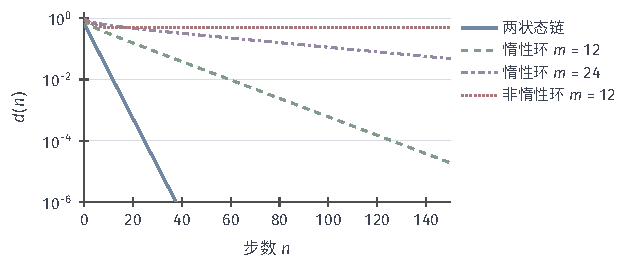
\includegraphics[width=106mm]{figures/03-optimization-evolution-and-signals/02-processes-and-trajectory-evolution/tikz/dtsp-tv-decay/figure.pdf}
  \caption{最坏初态到平稳分布的总变差$d(n)$（精确计算，纵轴对数刻度）。两状态链为$\frac23\times0.7^n$；惰性环每步以$1/2$停留、各以$1/4$移向两个邻点，$m$为环上状态数；非惰性环各以$1/2$移向两个邻点，$m=12$时周期为$2$，$d(n)$恒为$1/2$。}
  \label{fig:dtsp-tv-decay}
\end{figure}

\paragraph{谱的视角}
Dobrushin系数给出的速度常常保守。对可逆链，转移矩阵的谱给出更精细的刻画。在加权内积$\langle f,g\rangle_\pi=\sum_i\pi_if(i)g(i)$下，细致平衡等价于$\langle Pf,g\rangle_\pi=\langle f,Pg\rangle_\pi$，即$P$是自伴算子，因此特征值都是实数，可排为$1=\lambda_1\geq\lambda_2\geq\cdots\geq\lambda_{|E|}\geq-1$。

\begin{theorem}[可逆链的谱界]
  \label{thm:dtsp-spectral-bound}
  设有限链不可约且关于$\pi$可逆，$\lambda_\ast=\max\{|\lambda|:\lambda\text{为特征值},\lambda\neq1\}$。则对每个状态$x$，
  \[
    \lVert P^n(x,\cdot)-\pi\rVert_{\mathrm{TV}}\leq\frac12\sqrt{\frac{1-\pi_x}{\pi_x}}\,\lambda_\ast^n.
  \]
\end{theorem}

\begin{proof}
令$h_n(y)=P^n(x,y)/\pi_y$。由细致平衡，$h_n=P^nh_0$，其中$h_0=\mathbb I_{\{x\}}/\pi_x$；并且$h_0-1$与常数函数在$\langle\cdot,\cdot\rangle_\pi$下正交。$P$限制在与常数正交的子空间上范数为$\lambda_\ast$，故$\lVert h_n-1\rVert_\pi=\lVert P^n(h_0-1)\rVert_\pi\leq\lambda_\ast^n\lVert h_0-1\rVert_\pi=\lambda_\ast^n\sqrt{(1-\pi_x)/\pi_x}$。最后由Cauchy--Schwarz，$2\lVert P^n(x,\cdot)-\pi\rVert_{\mathrm{TV}}=\sum_y\pi_y|h_n(y)-1|\leq\lVert h_n-1\rVert_\pi$。
\end{proof}

两状态链的另一个特征值是$0.7$；从状态$1$出发，界为$\frac12\sqrt{1/2}\times0.7^n\approx0.354\times0.7^n$，与精确值$0.333\times0.7^n$相差无几。惰性环的特征值为$\frac12(1+\cos(2\pi k/m))$，$\lambda_\ast=\frac12(1+\cos(2\pi/m))$，$m=12$与$m=24$时分别约为$0.933$与$0.983$；$1-\lambda_\ast$称为谱间隙，它约以$m^{-2}$缩小，与图~\ref{fig:dtsp-tv-decay}中的斜率比较一致。负特征值接近$-1$对应近似周期的振荡，加入停留概率可以把谱推到非负。

\paragraph{一般状态空间：漂移与小集}
状态连续时，没有“矩阵的某个幂全为正”可用，但上面的两个要素仍有对应物。一是\term{漂移条件}（drift condition）：存在函数$V\geq1$、常数$\lambda<1$、$b<\infty$与集合$C$，使
\[
  PV(x)\leq\lambda V(x)+b\,\mathbb I_C(x),
\]
即链在$C$外平均地被拉回来。二是$C$上的\term{小集}（small set）条件：存在$m\geq1$、$\beta>0$与概率测度$\nu$，使$P^m(x,\cdot)\geq\beta\nu(\cdot)$对所有$x\in C$成立，即从$C$中任一点出发，$m$步后的分布都包含一份共同的成分，耦合在每次回到$C$时都有至少$\beta$的机会成功。在这两项及适当的非周期条件下，链有唯一不变分布$\pi$，并且存在$r<1$与常数$K$，使$\lVert P^n(x,\cdot)-\pi\rVert_{\mathrm{TV}}\leq KV(x)r^n$\scite{math-meyn2009markov}。

用图~\ref{fig:dtsp-ar1-path-bundle}的递推核对这两项。取$V(x)=1+x^2$，则$PV(x)=1+\mathbb E(0.8x+\xi)^2=0.64V(x)+1.36$。在$C=\{|x|\leq2.6\}$之外$1.36\leq0.18V(x)$，所以$PV\leq0.82V+1.36\,\mathbb I_C$。在$C$上，$P(x,\cdot)$的密度$\varphi(y-0.8x)$不小于$\varphi(|y|+2.08)$，$\varphi$为标准正态密度，于是小集条件以$m=1$成立。因此这个递推几何遍历，与图中边缘分布迅速靠近$\mathcal N(0,1/0.36)$的观察一致。

\subsection{遍历平均与相关样本误差}
\label{sec:dtsp-ergodic-averages}
\label{sec:stoch-markov-long-run-average}

\paragraph{沿一条轨迹求平均}
模拟或监测通常只有一条长轨迹。我们希望用时间平均$\overline f_n=\frac1n\sum_{k=0}^{n-1}f(X_k)$近似$\pi(f)=\sum_i\pi_if(i)$，例如服务器长期处于拥堵状态的比例。困难在于各项彼此相关，不能直接套用独立同分布的大数定律。第~\ref{sec:dtsp-strong-markov}节的再生分段提供了出路：把轨迹在每次回到某个固定状态处切开，各段游程独立同分布，于是可以对“段”而不是对“步”使用大数定律。

\begin{theorem}[Markov链的遍历定理]
  \label{thm:dtsp-ergodic-theorem}
  设可数状态链不可约且正常返。则它有唯一的不变分布$\pi$，$\pi_i=1/m_i$；并且对任意初始分布和任意满足$\pi(|f|)<\infty$的$f$，
  \begin{equation}
    \frac1n\sum_{k=0}^{n-1}f(X_k)\longrightarrow\pi(f)\qquad\text{几乎必然}.
    \label{eq:dtsp-ergodic-average}
  \end{equation}
  特别地，有限不可约链（无论是否周期）都满足此结论。
\end{theorem}

\begin{proof}
固定状态$i$，先设$X_0=i$、$f\geq0$。记第$r$次返回$i$的时刻为$T^{(r)}$，$T^{(0)}=0$，常返性保证它们都有限。令$L_r=T^{(r)}-T^{(r-1)}$为第$r$段游程的长度，$F_r=\sum_{k=T^{(r-1)}}^{T^{(r)}-1}f(X_k)$为该段的累计值。由强Markov性质，$(L_r,F_r)_{r\geq1}$独立同分布，$\mathbb E_iL_1=m_i<\infty$。

第一步，识别段内平均。令$a_j=\mathbb E_i\sum_{k<T_i^{+}}\mathbb I\{X_k=j\}$为一段游程中访问$j$的平均次数，则$\sum_ja_j=m_i$，且由非负项换序，$\mathbb E_iF_1=\sum_ja_jf(j)$。向量$a$满足平衡方程：事件$\{k<T_i^+\}$属于$\mathcal F_k$，逐项对$\mathcal F_k$取条件期望，
\[
  \sum_\ell a_\ell P_{\ell,j}=\mathbb E_i\sum_{k=0}^{T_i^+-1}P_{X_k,j}=\mathbb E_i\sum_{k=0}^{T_i^+-1}\mathbb I\{X_{k+1}=j\}=\mathbb E_i\sum_{k=1}^{T_i^+}\mathbb I\{X_k=j\}=a_j,
\]
最后一步因为$X_0=X_{T_i^+}=i$，把计数区间平移一格不改变总数。所以$\tilde\pi=a/m_i$是不变分布，且$\mathbb E_iF_1=m_i\tilde\pi(f)$。

第二步，对游程使用强大数定律。若$\tilde\pi(f)<\infty$，则$\frac1R\sum_{r\leq R}F_r\to m_i\tilde\pi(f)$，$\frac1RT^{(R)}\to m_i$，几乎必然。记$R(n)$为时刻$n$之前完成的游程数，$T^{(R(n))}\leq n<T^{(R(n)+1)}$，且$R(n)\to\infty$。由$f\geq0$，
\[
  \frac{\sum_{r\leq R(n)}F_r}{T^{(R(n)+1)}}\leq\frac1n\sum_{k=0}^{n-1}f(X_k)\leq\frac{\sum_{r\leq R(n)+1}F_r}{T^{(R(n))}},
\]
两侧都趋于$\tilde\pi(f)$，因为$T^{(R+1)}/T^{(R)}\to1$。

第三步，推广。对一般初态$j$，链几乎必然在有限时间内到达$i$：否则从$i$出发以正概率到达$j$后永不返回，与$i$常返矛盾。到达前的有限段除以$n$后趋于零。对一般初始分布按$X_0$的取值分解，对$\tilde\pi$可积的一般$f$分成正负部分。

第四步，唯一性与$\pi_i=1/m_i$。若$\rho$是任一不变分布，令链从$\rho$出发；对有界$f$，$\mathbb E_\rho\overline f_n=\rho(f)$，而由已证结论$\overline f_n\to\tilde\pi(f)$几乎必然，有界收敛给出$\rho(f)=\tilde\pi(f)$。所以$\rho=\tilde\pi$，不变分布唯一，记作$\pi$。取$f=\mathbb I_{\{i\}}$，每段游程恰好访问$i$一次，$F_r=1$，得$\pi_i=1/m_i$。有限不可约链由第~\ref{sec:dtsp-communication}节为正常返，故适用。
\end{proof}

定理没有要求非周期，这正是图~\ref{fig:dtsp-two-state-distribution}(b)中交替链的时间平均趋于$1/2$的原因：时间平均只需要回返，逐时刻分布收敛还需要非周期。公式$\pi_i=1/m_i$说长期停留比例等于平均返回时间的倒数：两状态链中$m_1=3/2$、$m_2=3$，与$\pi=(2/3,1/3)$一致。一般状态空间中，正Harris常返链对任意初态和$\pi$可积的$f$有同样的结论\scite{math-meyn2009markov}；仅以正概率到达或只有局部可积，都不足以推出它。

\paragraph{平稳过程的遍历定理}
对一般的平稳过程（不必是Markov链），也有时间平均的极限定理：若$(X_n)$严格平稳且$\mathbb E|f(X_0)|<\infty$，则$\overline f_n$几乎必然收敛，但极限一般是随机的，等于$f(X_0)$对“平移不变事件”所成$\sigma$代数的条件期望；只有当所有平移不变事件的概率为$0$或$1$（称过程遍历）时，极限才是常数$\mathbb Ef(X_0)$\scite{math-kallenberg2021probability}。图~\ref{fig:dtsp-communicating-classes}的链提供了不遍历的例子：若初态随机地落在$\{3,4\}$或$\{5,6\}$中，由于两个类都封闭，长期平均取决于落在哪一个类，是一个随机极限。Markov链遍历定理中的不可约性正是排除这种情形的条件。

\paragraph{相关样本平均的方差}
遍历定理说明时间平均对准了$\pi(f)$；现在问有限$n$下误差有多大。设链从$\pi$启动，$\sigma_f^2=\operatorname{Var}_\pi f(X_0)\in(0,\infty)$，自相关$\rho_f(k)=\operatorname{Corr}_\pi(f(X_0),f(X_k))$。由平稳性，$\operatorname{Cov}(f(X_j),f(X_k))=\sigma_f^2\rho_f(|j-k|)$，展开平方并把相同间隔的项合并，
\begin{equation}
  \operatorname{Var}\bigl(\overline f_n\bigr)=\frac{\sigma_f^2}{n}\Bigl[1+2\sum_{k=1}^{n-1}\Bigl(1-\frac kn\Bigr)\rho_f(k)\Bigr].
  \label{eq:dtsp-average-variance}
\end{equation}
若$\sum_k|\rho_f(k)|<\infty$，方括号趋于$\tau_f=1+2\sum_{k\geq1}\rho_f(k)$，称为积分自相关时间。于是$n$个相关样本的平均，其方差约等于$n/\tau_f$个独立样本的平均，$n/\tau_f$称为\term{自相关有效样本量}（autocorrelation effective sample size）。它是针对特定$f$的方差换算口径，不是链中“真正独立”的样本条数；自相关为负时$\tau_f$还可能小于一。

对两状态链取$f=\mathbb I\{X=2\}$。$f-\pi(f)$在$\{1,2\}$上取$(-1/3,2/3)$，正比于特征向量$(1,-2)^{\top}$，所以$P(f-\pi f)=0.7(f-\pi f)$，从而$\rho_f(k)=0.7^k$，并且
\[
  \sigma_f^2=\frac13\cdot\frac23=\frac29,\qquad\tau_f=1+2\sum_{k\geq1}0.7^k=\frac{1.7}{0.3}=\frac{17}{3}.
\]
一条长$n$的轨迹提供的信息只相当于约$3n/17$个独立观测。图~\ref{fig:dtsp-ergodic-average}(a)中十条从状态$1$出发的轨迹的时间平均都收进$\frac13\pm2\sqrt{(2/9)(17/3)/n}$的带内，$n=4000$时带宽约为$\pm0.035$；(b)中长轨迹的经验自相关与$0.7^k$吻合。

\begin{figure}[htbp]
  \centering
  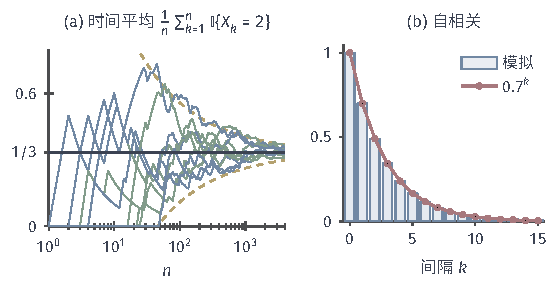
\includegraphics[width=94mm]{figures/03-optimization-evolution-and-signals/02-processes-and-trajectory-evolution/tikz/dtsp-ergodic-average/figure.pdf}
  \caption{两状态链的时间平均与自相关。(a)从状态$1$出发的$10$条模拟轨迹上，拥堵比例$\frac1n\sum_{k\leq n}\mathbb I\{X_k=2\}$随$n$的变化（横轴对数刻度）；黄色虚线为$\frac13\pm2\sqrt{\sigma_f^2\tau_f/n}$，$\sigma_f^2=2/9$、$\tau_f=17/3$。(b)一条长$200000$的模拟轨迹的经验自相关（柱）与精确值$0.7^k$（红线）。}
  \label{fig:dtsp-ergodic-average}
\end{figure}

\paragraph{Markov链的中心极限定理}
方差公式给出误差的尺度，误差的分布形状则需要中心极限定理。独立同分布情形的中心极限定理，以及用一致估计的标准误代替真值时的Slutsky定理，可参考\BookChapterRef{chap:weak-convergence-limit-theorems}{卷二“分布弱收敛、紧性与极限定理”章}。相关情形的关键一步，是把相关的和改写成鞅差的和。

对有限不可约链，方程
\begin{equation}
  g-Pg=f-\pi(f)
  \label{eq:dtsp-poisson-equation}
\end{equation}
有解$g$，称为链的\term{Poisson方程}（Poisson equation）。非周期时可以直接写出$g=\sum_{k\geq0}P^k(f-\pi f)$，定理~\ref{thm:dtsp-finite-convergence}保证级数几何收敛；周期情形也有解，只是需要另外构造。有了$g$，把$f(X_k)-\pi f=g(X_k)-Pg(X_k)$代入并重新配对，
\[
  \sum_{k=0}^{n-1}\bigl(f(X_k)-\pi f\bigr)=\sum_{k=1}^{n}\bigl(g(X_k)-Pg(X_{k-1})\bigr)+g(X_0)-g(X_n).
\]
右侧第一项的每一项给定$\mathcal F_{k-1}$均值为零，是有界鞅差的和；后两项有界，除以$\sqrt n$后消失。于是相关和的波动被归结为一个鞅的波动。对这个鞅使用鞅中心极限定理\scite{math-kallenberg2021probability}，得到：

\begin{theorem}[有限链的中心极限定理]
  \label{thm:dtsp-markov-clt}
  设有限链不可约，$g$满足式~\eqref{eq:dtsp-poisson-equation}。则对任意初始分布，
  \[
    \sqrt n\bigl(\overline f_n-\pi(f)\bigr)\xrightarrow{\ \mathrm d\ }\mathcal N(0,\sigma_{\mathrm{as}}^2),\qquad
    \sigma_{\mathrm{as}}^2=\pi(g^2)-\pi\bigl((Pg)^2\bigr).
  \]
  若链还非周期，则
  \[
    \sigma_{\mathrm{as}}^2=\sigma_f^2\tau_f=\operatorname{Var}_\pi f(X_0)+2\sum_{k\geq1}\operatorname{Cov}_\pi(f(X_0),f(X_k)) .
  \]
\end{theorem}

两状态链中$g=(f-\pi f)/0.3$，$Pg=0.7g$，于是$\sigma_{\mathrm{as}}^2=(1-0.49)\,\pi(g^2)=\frac{0.51}{0.09}\cdot\frac29\approx1.259$，与$\sigma_f^2\tau_f=\frac29\cdot\frac{17}3$一致。一般状态空间中，CLT需要比遍历定理更多的条件，例如几何遍历加上$f$的适当矩条件，或者Poisson方程有满足矩界的解；遍历律本身不蕴含CLT，经验有效样本量和自相关图等诊断也不能替代这些条件。第~\ref{sec:dtsp-mcmc}节在采样中使用这里的误差尺度，第~\ref{sec:dtsp-ode-markov}节则再次使用Poisson方程处理带Markov噪声的递推。

\section{随机采样与积分计算}
\label{sec:dtsp-sampling}

本节把前面的工具用于一个计算任务：近似一个固定的积分
\[
  I=\int_Ef\,\mathrm d\pi=\mathbb E_\pi f(X).
\]
被积分布$\pi$可能只知道到一个归一化常数为止，例如给定一组已经观测到的数据后，参数的后验密度正比于“先验密度乘以似然”，而比例常数本身就是一个难算的积分。思路是生成一列随机样本，使它们的平均接近$I$。样本可以相互独立，也可以来自一条以$\pi$为不变分布的Markov链；无论状态是实数还是向量，样本按编号排成的都是离散时间随机序列。我们依次讨论样本怎样生成、各样本的贡献怎样加权、误差怎样评估。这里研究的是数值计算误差：$I$作为统计量有什么含义、怎样从数据推断，由统计推断部分说明。

\subsection{独立采样与样本平均}
\label{sec:dtsp-iid-sampling}

\paragraph{从均匀随机数到指定分布}
计算机能直接产生的是$(0,1)$上的均匀随机数（更准确地说，是通过统计检验的伪随机数）。其他分布都要由它变换而来。最直接的变换是把累积分布函数“倒过来用”。对实值分布函数$F$，定义广义逆$F^{-1}(u)=\inf\{x:F(x)\geq u\}$。

\begin{theorem}[逆变换采样]
  \label{thm:dtsp-inverse-transform}
  若$U\sim\operatorname{Unif}(0,1)$，则$X=F^{-1}(U)$的分布函数为$F$。
\end{theorem}

\begin{proof}
$F$右连续且单调不减，所以$\{x:F(x)\geq u\}$是一个包含左端点的区间$[F^{-1}(u),\infty)$。于是$F^{-1}(u)\leq x$当且仅当$u\leq F(x)$，从而$\mathbb P(X\leq x)=\mathbb P(U\leq F(x))=F(x)$。
\end{proof}

图~\ref{fig:dtsp-inverse-rejection}(a)用指数分布演示这一步：在纵轴上取均匀数$u$，水平走到曲线$F(x)=1-e^{-x}$，再竖直落到横轴，得到$x=-\log(1-u)$。曲线陡的地方，纵轴上的一小段对应横轴上的一小段，样本密集；曲线平的地方样本稀疏，正好对应密度的高低。离散分布同样适用：把概率依次累加，看$u$落在哪一段。这个方法要求能够计算$F^{-1}$，多维分布一般做不到。

\paragraph{拒绝采样}
若只能计算目标密度$p$（甚至只知道它的常数倍），却能从另一个密度$g$采样，且$p\leq Mg$对某个常数$M$成立，可以“先多抽，再筛掉”。把$Mg$的图像想成罩在$p$外面的帐篷：在帐篷下均匀撒点，只保留落在$p$曲线下方的点，这些点的横坐标就服从$p$。具体步骤是：抽取$Y\sim g$与独立的$U\sim\operatorname{Unif}(0,1)$；若$U\leq p(Y)/(Mg(Y))$则输出$Y$，否则重来。

\begin{theorem}[拒绝采样]
  \label{thm:dtsp-rejection}
  在上述条件下，每轮被接受的概率为$1/M$，所需轮数服从均值为$M$的几何分布，输出的样本密度为$p$。
\end{theorem}

\begin{proof}
对可测集$B$，
\[
  \mathbb P(Y\in B,\ \text{接受})=\int_Bg(y)\frac{p(y)}{Mg(y)}\,\mathrm dy=\frac1M\int_Bp(y)\,\mathrm dy.
\]
取$B$为全空间得接受概率$1/M$；两式相除得到接受条件下$Y$的分布为$p$。各轮独立，所以轮数服从几何分布。
\end{proof}

若只知道$\tilde p=Zp$且$\tilde p\leq\tilde Mg$，算法照样执行，接受概率变为$Z/\tilde M$，未知常数$Z$不需要算出。图~\ref{fig:dtsp-inverse-rejection}(b)从均匀分布中为密度$6x(1-x)$采样，帐篷高度取其最大值$M=1.5$，理论接受率为$2/3$；图中$260$个候选点接受了$167$个。拒绝采样的代价在高维中急剧上升。用$d$维立方体$[-1,1]^d$罩住单位球、在球内均匀采样，接受率是体积比$\pi^{d/2}/(\Gamma(d/2+1)2^d)$：$d=2$时为$0.785$，$d=10$时只有约$0.0025$，平均要试四百次才得到一个样本。

\begin{figure}[htbp]
  \centering
  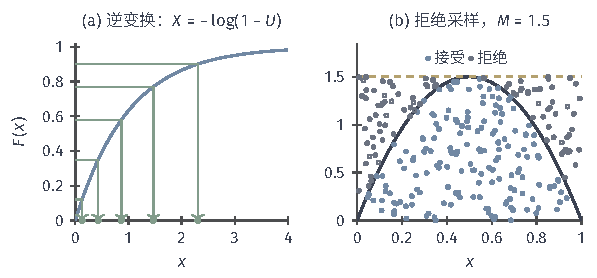
\includegraphics[width=101mm]{figures/03-optimization-evolution-and-signals/02-processes-and-trajectory-evolution/tikz/dtsp-inverse-rejection/figure.pdf}
  \caption{由均匀随机数生成样本。(a)逆变换：纵轴上的五个均匀数$u$沿绿线经指数分布函数$F(x)=1-e^{-x}$映到横轴上的样本$-\log(1-u)$；(b)拒绝采样：在高度$M=1.5$的均匀“帐篷”下撒$260$个点（固定随机种子），落在密度$6x(1-x)$下方的点（实心）被接受，其横坐标服从该密度。}
  \label{fig:dtsp-inverse-rejection}
\end{figure}

\paragraph{样本平均与Monte Carlo积分}
有了独立样本$X_1,\ldots,X_n\sim\pi$，最自然的估计是样本平均
\[
  \widehat I_n=\frac1n\sum_{i=1}^nf(X_i),
\]
称为\term{Monte Carlo积分}（Monte Carlo integration）。若$\pi(|f|)<\infty$，它无偏；若$\sigma^2=\operatorname{Var}_\pi f(X)<\infty$，则$\operatorname{Var}(\widehat I_n)=\sigma^2/n$。对它要分清三种不同的误差陈述。一致性：由强大数律，$\widehat I_n\to I$几乎必然，只需要$\pi(|f|)<\infty$。均方误差：$\mathbb E(\widehat I_n-I)^2=\sigma^2/n$是精确等式，需要$\sigma^2<\infty$。数值标准误：实际计算时$\sigma^2$未知，用样本方差$\widehat\sigma^2_n$代替，报告$\widehat\sigma_n/\sqrt n$；由中心极限定理与Slutsky定理，在$0<\sigma^2<\infty$时$\widehat I_n\pm1.96\,\widehat\sigma_n/\sqrt n$渐近地以$95\%$的概率覆盖$I$。前两条是关于估计量的性质，第三条是对误差大小的数值估计，它本身也有误差。

以$I=\int_0^1x^2\,\mathrm dx=1/3$为贯穿例子，$X\sim\operatorname{Unif}(0,1)$，$f(x)=x^2$，单样本方差$\sigma^2=\frac15-\frac19=\frac4{45}$。$n=10^4$时标准误约为$0.003$。图~\ref{fig:dtsp-monte-carlo-rate}(a)在双对数坐标上画出十二次独立运行的绝对误差，它们围绕斜率为$-1/2$的直线$\sqrt{4/(45n)}$上下起伏；(b)显示$n=400$时缩放误差$\sqrt n(\widehat I_n-I)$的直方图与$\mathcal N(0,4/45)$密度吻合。

\begin{figure}[htbp]
  \centering
  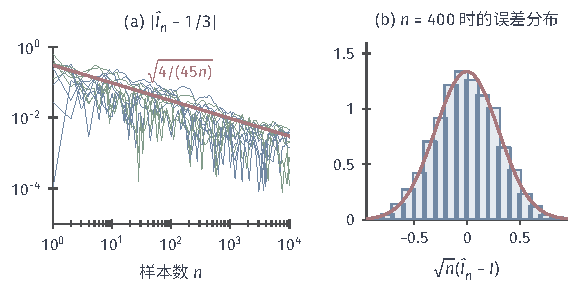
\includegraphics[width=97mm]{figures/03-optimization-evolution-and-signals/02-processes-and-trajectory-evolution/tikz/dtsp-monte-carlo-rate/figure.pdf}
  \caption{Monte Carlo积分$\int_0^1x^2\,\mathrm dx$的误差。(a)$12$次独立运行的$|\widehat I_n-1/3|$（双对数坐标），红线为均方根误差$\sqrt{4/(45n)}$；(b)$n=400$时$3000$次重复的$\sqrt n(\widehat I_n-I)$直方图，红线为$\mathcal N(0,4/45)$密度。}
  \label{fig:dtsp-monte-carlo-rate}
\end{figure}

\paragraph{维数的作用}
$n^{-1/2}$的速度与被积变量的维数$d$无关，这是Monte Carlo相对于网格求积的主要优势：网格方法在$d$维中用$n$个点，每个方向只有$n^{1/d}$个点，精度随$d$急剧下降。但“与维数无关”只针对指数，不针对常数。设$X$在$[0,1]^d$上均匀，估计$p=\mathbb P(\text{所有坐标}\leq0.9)=0.9^d$。单样本相对标准差是$\sqrt{(1-p)/p}$；$d=50$时$p\approx0.0052$，相对标准差约$13.9$，要把相对误差压到$1\%$需要约$1.9\times10^6$个样本。维数通过方差$\sigma^2$和每个样本的生成成本进入计算量。下面两小节的方法都着眼于在不改变$I$的前提下减小$\sigma^2$。

\subsection{重要性抽样与自归一化}
\label{sec:dtsp-importance}

\paragraph{换一个分布来抽样}
上面的例子中，大部分样本落在对积分毫无贡献的区域。若改从另一个分布$q$抽样，让样本更多地落在$|f|p$大的地方，再给每个样本乘一个修正权重，就可能在保持期望的同时降低方差。设$\pi$与$q$关于同一参考测度分别有密度$p,q$，并且
\begin{equation}
  q(x)>0\quad\text{在}\ \{x:f(x)p(x)\neq0\}\ \text{上几乎处处成立}.
  \label{eq:dtsp-is-support}
\end{equation}
记$w=p/q$（在$q>0$处定义），则$I=\int fp=\int(fw)q=\mathbb E_q[f(X)w(X)]$。当$\pi\ll q$时，$w$就是Radon--Nikodym导数$\mathrm d\pi/\mathrm dq$，换测度公式可参考\BookChapterRef{chap:densities-change-of-measure}{卷二“密度与换测度”章}。由此得到\term{重要性抽样}（importance sampling）估计
\begin{equation}
  \widehat I_n^{\mathrm{IS}}=\frac1n\sum_{i=1}^nw(X_i)f(X_i),\qquad X_i\ \text{独立同分布于}\ q.
  \label{eq:dtsp-importance-sampling}
\end{equation}
它无偏，只要$\mathbb E_q|fw|<\infty$；其方差为$\frac1n(\mathbb E_q[f^2w^2]-I^2)$，有限二阶矩$\mathbb E_q[f^2w^2]<\infty$是一项额外要求。支撑条件~\eqref{eq:dtsp-is-support}不能省略：若$q$在$fp$有质量的区域为零，那里永远采不到样本，估计量对准的就不是$I$。

仍以$\int_0^1x^2\,\mathrm dx$为例，取$q(x)=2x$，则$w(x)=1/(2x)$，$f(x)w(x)=x/2$，单样本方差为$\mathbb E_q[X^2/4]-\frac19=\frac18-\frac19=\frac1{72}$，比直接平均的$4/45$小六倍多。这次改进来自$q$把样本更多地放在$x^2$大的地方。

\paragraph{最优提议与重尾风险}
什么样的$q$最好？由Cauchy--Schwarz不等式，在满足条件~\eqref{eq:dtsp-is-support}的密度中，
\[
  \Bigl(\int|f|p\Bigr)^2=\Bigl(\int_{\{q>0\}}\frac{|f|p}{\sqrt q}\sqrt q\Bigr)^2\leq\int\frac{f^2p^2}{q}=\mathbb E_q[f^2w^2],
\]
等号当且仅当$q\propto|f|p$。所以二阶矩最小的提议是$q^\star=|f|p/\int|f|p$；若$f\geq0$，此时$fw\equiv I$，方差为零。这个理想提议通常不能直接使用，因为它的归一化常数就是要算的积分；但它指明了方向：提议应当在$|f|p$大的地方有足够的质量，尾部不能比$|f|p$轻。

尾部过轻的后果可以精确算出。取目标$p=\mathcal N(0,1)$、$f\equiv1$，提议$q=\mathcal N(0,s^2)$，则$w(x)=s\exp\bigl(x^2(s^{-2}-1)/2\bigr)$，
\[
  \mathbb E_qw^2=\int\frac{p^2}{q}=\frac{s^2}{\sqrt{2s^2-1}}\qquad(s^2>1/2),
\]
而$s^2\leq1/2$时积分发散。图~\ref{fig:dtsp-importance-variance}(a)画出这条曲线：$s=1$时为$1$，偏离$1$时增大，越过$1/\sqrt2$后变为无穷。方差无穷时估计量仍然无偏、仍然几乎必然收敛，但它的误差不再按$n^{-1/2}$规律下降，常常表现为长时间平稳后被一个巨大权重突然推开；图(b)中$s=0.6$的运行在前几十个样本内就出现了这样的跳跃，而$s=1.6$的运行平稳得多。

\begin{figure}[htbp]
  \centering
  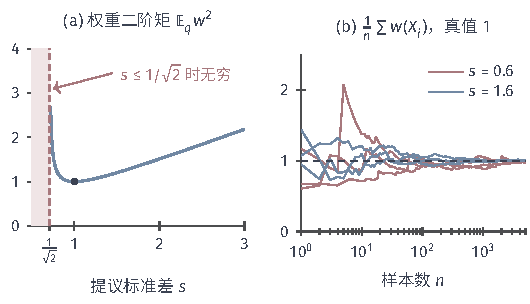
\includegraphics[width=90mm]{figures/03-optimization-evolution-and-signals/02-processes-and-trajectory-evolution/tikz/dtsp-importance-variance/figure.pdf}
  \caption{提议尾部与重要性权重的方差。目标为$\mathcal N(0,1)$，提议为$\mathcal N(0,s^2)$，权重$w=p/q$，估计对象为$\mathbb E_qw=1$。(a)精确的二阶矩$\mathbb E_qw^2=s^2/\sqrt{2s^2-1}$，在$s\leq1/\sqrt2$（阴影）时为无穷；(b)$s=0.6$与$s=1.6$各三次运行的累计平均（横轴对数刻度，固定随机种子）。}
  \label{fig:dtsp-importance-variance}
\end{figure}

反过来，选得好的提议可以把方差降低几个数量级。估计罕见事件概率$p_4=\mathbb P(Z>4)\approx3.17\times10^{-5}$，$Z\sim\mathcal N(0,1)$。直接平均示性函数时，单样本相对方差为$(1-p_4)/p_4\approx3.2\times10^4$。改从$\mathcal N(4,1)$抽样，权重为$e^{-4x+8}$，二阶矩为
\[
  \int_4^\infty\varphi(x)e^{-4x+8}\,\mathrm dx=e^{16}\int_4^\infty\varphi(x+4)\,\mathrm dx=e^{16}\,\mathbb P(Z>8)\approx5.5\times10^{-9},
\]
其中$\varphi$是标准正态密度。相对方差降为$5.5\times10^{-9}/p_4^2-1\approx4.5$。同样的精度所需样本数缩小约七千倍。

\paragraph{只知道未归一化密度}
很多目标只知道$\tilde p=Zp$，常数$Z$未知，于是权重$w$也只知道常数倍$\tilde w=\tilde p/q=Zw$。把加权和除以权重和，未知常数就约掉了：
\begin{equation}
  \widehat I_n^{\mathrm{SN}}=\frac{\sum_{i=1}^n\tilde w(X_i)f(X_i)}{\sum_{i=1}^n\tilde w(X_i)}.
  \label{eq:dtsp-self-normalized-is}
\end{equation}
这称为自归一化重要性抽样。若$\mathbb E_q|f\tilde w|<\infty$，强大数律给出分子$/n\to ZI$、分母$/n\to Z$几乎必然，所以$\widehat I_n^{\mathrm{SN}}\to I$几乎必然。但它是两个随机量之比，一般有偏，因为$\mathbb E[A/B]\neq\mathbb EA/\mathbb EB$；偏差的量级为$O(1/n)$。把比值在$(ZI,Z)$附近线性化，可以得到它的渐近方差约为$\frac1n\mathbb E_q[w^2(f-I)^2]$：与$f$本身相比，起作用的是中心化后的$f-I$。

自归一化之外，实践中常见的两个修补都有代价。设三点空间上$q=(0.8,0.15,0.05)$、$p=(0.4,0.3,0.3)$，则$w=(0.5,2,6)$；对$f=(0,1,1)$，$I=0.6$，单样本贡献$wf=(0,2,6)$的方差为$0.15\times4+0.05\times36-0.36=2.04$。若把权重截断在$2$，方差降到$0.64$，但均值变成$0.4$，引入了$-0.2$的偏差，截断必须连同偏差一起报告。若按归一化权重重采样，样本被复制成等权粒子，权重不均的问题在后续计算中得到缓解，却增加了额外的随机性。常用的诊断量$\widehat n_{\mathrm{eff}}=(\sum_i\tilde w_i)^2/\sum_i\tilde w_i^2$度量权重退化的程度，它不是严格意义上的独立样本数，也不能说明偏差已经消失。还应注意，这里的“自归一化”指用权重和作分母，与第~\ref{sec:dtsp-maximal-tail}节用设计矩阵归一化累计噪声不是同一个概念。

\subsection{固定积分的方差缩减}
\label{sec:dtsp-variance-reduction}

本小节的方法都保持积分目标不变，只改变样本贡献的写法或样本之间的搭配。比较时要固定同一个积分和同样的计算预算（例如被积函数的求值次数），再比较方差与额外的计算或先验信息。

\paragraph{控制变量}
若手头有一个与$f(X)$一起波动、且均值$\mu_h$已知的辅助量$h(X)$，可以减去它偏离均值的部分。对任意常数$\beta$，$f_\beta=f-\beta(h-\mu_h)$的期望仍是$I$，方差为$\operatorname{Var}f-2\beta\operatorname{Cov}(f,h)+\beta^2\operatorname{Var}h$。对$\beta$求最小，得到
\[
  \beta^\star=\frac{\operatorname{Cov}(f,h)}{\operatorname{Var}h},\qquad
  \operatorname{Var}f_{\beta^\star}=(1-\rho_{f,h}^2)\operatorname{Var}f,
\]
其中$\rho_{f,h}$是二者的相关系数：相关越强，剩下的方差越少。对$f(x)=x^2$、$h(x)=x$、$X\sim\operatorname{Unif}(0,1)$，$\mu_h=1/2$，$\operatorname{Cov}(X^2,X)=\frac14-\frac16=\frac1{12}$，$\operatorname{Var}X=\frac1{12}$，于是$\beta^\star=1$，调整后的被积量$x^2-x+\frac12$方差为$\frac1{180}$，是原来的$1/16$。实际中$\beta^\star$也要从同一批样本估计；这时估计量不再严格无偏，误差公式也要计入系数的随机性，只是大样本下这一影响是高阶的。

\paragraph{条件平均}
若估计过程中抽取了对目标不必要的额外随机量，可以把它积分掉。设$Y$是$I$的无偏估计，$\mathbb EY^2<\infty$，$T$是某个能直接计算条件期望的统计量，令$Y^\star=\mathbb E[Y\mid T]$。塔式性质给出$\mathbb EY^\star=I$，全方差公式给出
\[
  \operatorname{Var}Y=\mathbb E[\operatorname{Var}(Y\mid T)]+\operatorname{Var}Y^\star\geq\operatorname{Var}Y^\star.
\]
这称为\term{Rao--Blackwell化}（Rao--Blackwellization）。例如在单位正方形中撒点、数落在曲线$u=x^2$下方的比例（命中法）：$Y=\mathbb I\{U\leq X^2\}$，$\operatorname{Var}Y=\frac13\cdot\frac23=\frac29$。对$X$取条件期望，$\mathbb E[Y\mid X]=X^2$，正是直接平均，方差降为$4/45$。图~\ref{fig:dtsp-rao-blackwell}把条件平均解释为竖切片上命中区段的长度：给定$X=0.6$，再抽一次$U$只会得到$0$或$1$，而它的条件均值$0.36$可以直接算出。

\begin{figure*}[htbp]
  \centering
  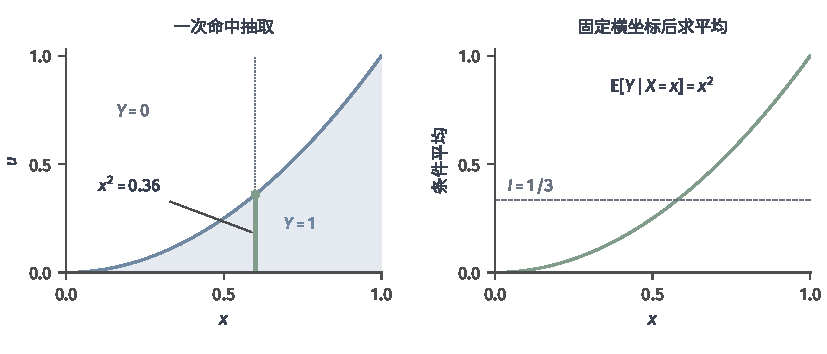
\includegraphics[width=140mm]{figures/00-shared/mathematical-preliminaries-lower/01-random-variables-distributions-and-causality/matplotlib/probability-rao-blackwell-slice/figure.pdf}
  \caption{命中积分的Rao--Blackwell化（解析式教学图）。独立的$X,U$均在$(0,1)$上均匀分布。左图阴影为$U\leq X^2$，竖切片$x=0.6$的命中长度为$0.36$；右图保留每个$x$对应的条件均值$x^2$。两个估计量的期望均为$1/3$，单样本方差分别为$2/9$与$4/45$。}
  \label{fig:dtsp-rao-blackwell}
\end{figure*}

\paragraph{对偶变量}
上面两种方法改造单个样本的贡献；另一类方法改变样本之间的搭配。若$f$单调，$X$与$1-X$给出的$f$值一大一小，把它们配成一对取平均，正负误差会部分抵消。一对的平均$\frac12(f(X)+f(1-X))$的方差为$\frac{\sigma^2}2(1+\rho)$，其中$\rho=\operatorname{Corr}(f(X),f(1-X))$；与两个独立样本的平均$\sigma^2/2$相比，$\rho<0$时有改进。对$f(x)=x^2$，一对的平均恰为$x^2-x+\frac12$，方差为$1/180$，按每次函数求值折算为$1/90$。改进依赖负相关，并非无条件成立：若$f(x)=(x-\frac12)^2$关于$\frac12$对称，则$f(X)=f(1-X)$，$\rho=1$，配对平均的方差是独立两样本的两倍。

\paragraph{分层采样}
另一种搭配方式是把样本按比例分配到各个区域。把$[0,1]$分成$K$个等长小区间，每个区间里各取$n/K$个均匀点，用各区间平均的加权和估计$I$。记第$j$层的条件方差为$\sigma_j^2$、层内均值为$\mu_j$，按比例分配时估计量的方差为$\frac1n\sum_j\frac1K\sigma_j^2$。由全方差公式，$\sigma^2=\sum_j\frac1K\sigma_j^2+\sum_j\frac1K(\mu_j-I)^2$，所以分层永远不会比直接平均差，并且去掉了层与层之间的波动。$K=10$、每层一个点时，$n\operatorname{Var}=0.0011$，在这个光滑一维例子中优于前面所有方法。分层的效果依赖于能否把空间切成层内变化小的区域；高维中层数随维数指数增长，必须改用更粗的分层或自适应分层。

图~\ref{fig:dtsp-variance-reduction}把这些方法放在同一个积分、同样的函数求值预算下比较。排序只对这一个光滑的一维积分成立：它展示的是各种方法起作用的机制与代价，不是对其他问题的普遍排名。重要性抽样需要能从$q$采样并计算密度比，控制变量需要已知的辅助均值，对偶变量需要单调性，分层需要能在每层内条件采样。

\begin{figure}[htbp]
  \centering
  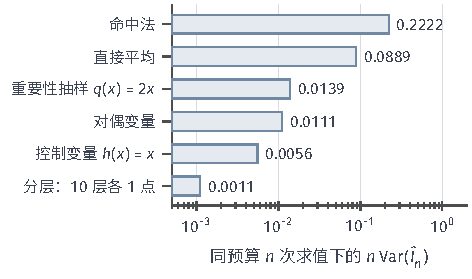
\includegraphics[width=80mm]{figures/03-optimization-evolution-and-signals/02-processes-and-trajectory-evolution/tikz/dtsp-variance-reduction/figure.pdf}
  \caption{同一积分$\int_0^1x^2\,\mathrm dx$在$n$次被积函数求值预算下的$n\operatorname{Var}(\widehat I_n)$（精确值，横轴对数刻度）。命中法为$2/9$，直接平均为$4/45$，对偶变量按每次求值折算为$1/90$，重要性抽样（$q(x)=2x$）为$1/72$，控制变量（$h(x)=x$，$\beta=1$）为$1/180$，分层为十个等长层各取一点。}
  \label{fig:dtsp-variance-reduction}
\end{figure}

\subsection{Markov链采样}
\label{sec:dtsp-mcmc}

当$\pi$的维数高、形状复杂、只知道未归一化密度$\tilde\pi$时，逆变换、拒绝采样和简单的重要性抽样往往都不可行。换一个思路：不直接从$\pi$采样，而是设计一条以$\pi$为不变分布的Markov链，让它长时间运行，再用遍历定理把时间平均当作积分。第~\ref{sec:dtsp-reversibility}节说明，细致平衡是保证不变性的便利条件，它只涉及两个状态的密度比，未知的归一化常数自然约掉。这类方法统称为\term{Markov链蒙特卡洛}（Markov chain Monte Carlo）。

\paragraph{Metropolis--Hastings}
设$\pi$关于参考测度有密度，$\tilde\pi\propto\pi$可计算；$q(x,y)$是一个可以采样的提议密度。\term{Metropolis--Hastings方法}（Metropolis--Hastings）的一步是：在当前状态$x$处抽取候选$y\sim q(x,\cdot)$，以概率
\begin{equation}
  a(x,y)=\min\Bigl\{1,\ \frac{\tilde\pi(y)q(y,x)}{\tilde\pi(x)q(x,y)}\Bigr\}
  \label{eq:dtsp-mh-acceptance}
\end{equation}
接受并移到$y$，否则停在$x$\scite{pgm-history-metropolis1953,pgm-history-hastings1970}。停在原地也要记为一个样本，否则会改变链的不变分布。所得转移核为$P(x,\mathrm dy)=q(x,y)a(x,y)\,\mathrm dy+r(x)\delta_x(\mathrm dy)$，其中$r(x)=1-\int q(x,y)a(x,y)\,\mathrm dy$是拒绝概率。

\begin{theorem}[Metropolis--Hastings的细致平衡]
  \label{thm:dtsp-mh-balance}
  上述转移核关于$\pi$满足细致平衡，因而以$\pi$为不变分布。
\end{theorem}

\begin{proof}
对$x\neq y$，由式~\eqref{eq:dtsp-mh-acceptance}，
\[
  \pi(x)q(x,y)a(x,y)=\min\{\pi(x)q(x,y),\ \pi(y)q(y,x)\},
\]
右侧关于$x,y$对称，所以两点之间的正反流量相等。拒绝部分集中在对角线$\{y=x\}$上，在交换$x,y$时本身不变。两部分合起来就是式~\eqref{eq:dtsp-detailed-balance}，再由定理~\ref{thm:dtsp-detailed-balance}得到不变性。
\end{proof}

接受率只用到密度比$\tilde\pi(y)/\tilde\pi(x)$，归一化常数不需要知道。若提议对称，$q(x,y)=q(y,x)$（例如$y=x+\varepsilon$、$\varepsilon\sim\mathcal N(\bm 0,s^2\bm I)$），接受率化为$\min\{1,\tilde\pi(y)/\tilde\pi(x)\}$：往高密度处走一定接受，往低密度处走按比例接受。每一步只需一次提议和一次$\tilde\pi$求值。

\paragraph{从不变到可用}
细致平衡只保证“从$\pi$出发会留在$\pi$”。要让任意初态出发的时间平均收敛到$I$，还要第~\ref{sec:dtsp-long-run}节的回返条件。随机游走提议的密度处处为正时，链是$\pi$不可约的；只要拒绝以正概率发生，链就是非周期的；在这些条件下Metropolis--Hastings链是正Harris常返的，遍历定理适用\scite{math-meyn2009markov}。但这些定性条件不保证收敛得快。随机游走的步长$s$是关键：步长小，几乎总被接受，但每步只挪一点，路径像扩散一样缓慢；步长大，多数提议落到低密度区而被拒绝，链经常原地不动。两种情形的自相关都很高。

图~\ref{fig:dtsp-mh-gibbs}(a)对相关系数$0.95$的二维正态目标运行随机游走Metropolis--Hastings，$s=0.35$，长程接受率约$0.56$。目标的高密度区是一条细长的斜脊，提议在各方向同样大小，所以沿脊的移动只能靠许多小步累积；(c)中第一坐标的自相关在间隔$40$处仍约为$0.5$。

\paragraph{Gibbs采样}
另一种构造利用条件分布。设$x=(x_1,\ldots,x_d)$，若能从每个满条件分布$\pi(x_j\mid x_{-j})$中直接采样，就可以每次只更新一个坐标、其余坐标不动。这就是\term{Gibbs采样}（Gibbs sampling）\scite{pgm-history-geman1984}。单坐标更新核$K_j$保持$\pi$：若$X\sim\pi$，则$X_{-j}$服从$\pi$的边缘，再从$\pi(\cdot\mid X_{-j})$抽出新的第$j$坐标，联合分布仍是$\pi$。它也可以看成提议恰为满条件分布的Metropolis--Hastings，此时式~\eqref{eq:dtsp-mh-acceptance}中的比值恒为$1$，所以每个$K_j$都满足细致平衡。

把各坐标的更新组合起来有两种方式。按固定顺序依次更新（系统扫描），一轮的核是$K_1K_2\cdots K_d$；每个因子保持$\pi$，乘积也保持$\pi$，但乘积一般不再可逆。每轮随机选一个坐标更新（随机扫描），核为$\frac1d\sum_jK_j$，仍满足细致平衡。把强相关的坐标合成一块一起更新，称为分块Gibbs，往往比逐个坐标快得多。

对相关系数为$\rho$的标准二维正态，满条件分布为$x_1\mid x_2\sim\mathcal N(\rho x_2,1-\rho^2)$，另一个对称。系统扫描一轮后，第一坐标满足$x_1'=\rho^2x_1+\eta$，$\eta$与$x_1$独立，因此它是系数为$\rho^2$的一阶递推，自相关为$\rho^{2k}$，积分自相关时间为$(1+\rho^2)/(1-\rho^2)$。$\rho=0.95$时约为$19.5$。图~\ref{fig:dtsp-mh-gibbs}(b)中Gibbs路径只能沿坐标方向横竖移动，在斜脊上走出细碎的阶梯；(c)中它的自相关与$\rho^{2k}$吻合，衰减比随机游走快，但仍远慢于独立样本。

\begin{figure*}[htbp]
  \centering
  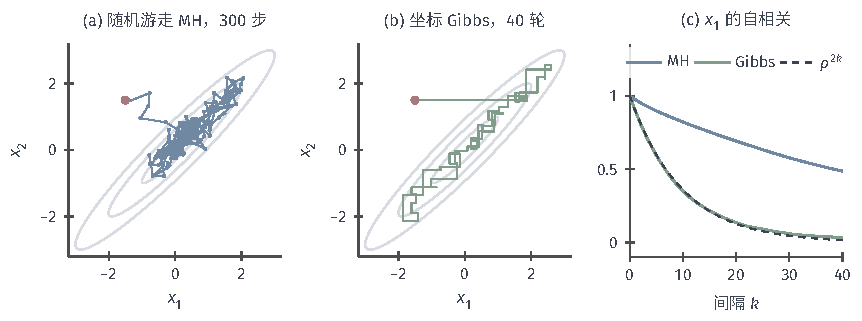
\includegraphics[width=146mm]{figures/03-optimization-evolution-and-signals/02-processes-and-trajectory-evolution/tikz/dtsp-mh-gibbs/figure.pdf}
  \caption{相关二维正态目标上的两种Markov链采样。目标方差均为$1$、相关系数$0.95$，灰色椭圆为马氏半径$1,2,3$的等高线，红点为共同初态$(-1.5,1.5)$。(a)随机游走Metropolis--Hastings，提议$\mathcal N(\bm 0,0.35^2\bm I)$，$300$步；(b)系统扫描坐标Gibbs，$40$轮（每轮先更新$x_1$再更新$x_2$）；(c)由长$60000$的运行估计的$x_1$自相关，虚线为Gibbs的精确值$\rho^{2k}$。}
  \label{fig:dtsp-mh-gibbs}
\end{figure*}

\paragraph{可运行与有效探索}
能运行、能保持$\pi$，不等于能把$\pi$走遍。设$\pi$是两个对角正方形$[0,1]^2\cup[1,2]^2$上的均匀分布。从左下方块出发，给定$x_2\in(0,1)$时$x_1$的满条件分布是$[0,1]$上的均匀分布，Gibbs采样永远到不了右上方块：链可约，时间平均只代表一半目标。即使链不可约，多峰目标也会让局部提议在一个峰附近停留极长时间，遍历定理虽然成立，有限预算内的平均却可能严重偏离。

\paragraph{相关样本的误差评估}
Markov链样本的误差有两个来源。一是初态偏差：链从任意初态出发，前若干步还没“忘记”起点；对几何遍历的链，它对时间平均的影响是$O(1/n)$，常见做法是丢弃一段初始样本。二是相关性：由第~\ref{sec:dtsp-ergodic-averages}节，时间平均的渐近方差为$\sigma_{\mathrm{as}}^2/n=\sigma_f^2\tau_f/n$，需要估计积分自相关时间而不是照搬$\sigma_f^2/n$。一种简单的估计方法是分批平均：把长度$n$的轨迹分成$b$批，每批长$\ell$，批平均的样本方差乘以$\ell$就估计$\sigma_{\mathrm{as}}^2$；批长与批数都要足够大。从分散的初态运行多条链、比较它们的平均与方差，可以暴露没有混合好的情形。这些诊断都只能发现问题，不能证明链已经收敛；收敛的证据来自第~\ref{sec:dtsp-long-run}节那类定理所需的条件。

\subsection{Hamilton轨迹生成的采样提议}
\label{sec:dtsp-hmc}

\paragraph{为什么要借助动量}
随机游走提议的问题在于它是“扩散”的：每一步随机选方向，走过距离$L$大约需要$(L/s)^2$步。在图~\ref{fig:dtsp-mh-gibbs}那样的细长目标上，步长$s$受窄方向限制，长方向就走得极慢。若能让提议沿着高密度区“滑行”一大段、而不是随机碰撞，相关性就会大大降低。Hamilton动力学提供了这样的滑行：把$-\log\pi$想成地形的高度，给一个小球随机的初速度，让它在无摩擦的地形上滚动一段时间，它会自然地沿着等高线附近的低谷走很远。

\paragraph{扩充状态与精确流}
设$\pi(\bm q)\propto e^{-U(\bm q)}$，$U$连续可微。引入与$\bm q$独立的动量$\bm p\sim\mathcal N(\bm 0,\bm M)$，$\bm M$对称正定，联合密度为
\[
  \rho(\bm q,\bm p)\propto e^{-H(\bm q,\bm p)},\qquad H(\bm q,\bm p)=U(\bm q)+\tfrac12\bm p^{\top}\bm M^{-1}\bm p.
\]
$\rho$对$\bm p$积分后恰为$\pi$，所以只要构造以$\rho$为不变分布的链，丢掉动量坐标就得到以$\pi$为不变分布的链。Hamilton方程$\dot{\bm q}=\bm M^{-1}\bm p$、$\dot{\bm p}=-\nabla U(\bm q)$的精确流$\Phi_t$有三项性质（见第~\ref{chap:ordinary-differential-equations}章）：它保持$H$不变；它保持相空间体积，因为向量场的散度$\nabla_{\bm q}\cdot(\bm M^{-1}\bm p)+\nabla_{\bm p}\cdot(-\nabla U)=0$；它在动量翻转$R(\bm q,\bm p)=(\bm q,-\bm p)$下可逆，即$R\Phi_tR=\Phi_{-t}$。于是$T=R\circ\Phi_t$是保体积的对合（$T^2$为恒等），并且$H(T\bm z)=H(\bm z)$，变量替换给出：若$\bm z\sim\rho$，则$T\bm z\sim\rho$。以$T\bm z$为提议，接受率为一。

\paragraph{蛙跳离散与接受校正}
精确流一般求不出来，要用数值积分代替。\term{蛙跳积分}（leapfrog integrator）的一步为
\[
  \bm p\leftarrow\bm p-\tfrac h2\nabla U(\bm q),\qquad
  \bm q\leftarrow\bm q+h\bm M^{-1}\bm p,\qquad
  \bm p\leftarrow\bm p-\tfrac h2\nabla U(\bm q).
\]
每个子步只改变一组坐标、改变量只依赖另一组坐标，是剪切映射，Jacobian行列式为$1$；三步对称排列，使一步映射$\Psi_h$满足$R\Psi_hR=\Psi_h^{-1}$。因此$T=R\circ\Psi_h^L$仍是保体积的对合。它唯一失去的是能量守恒：在固定的总时间$hL$上，能量误差为$O(h^2)$。图~\ref{fig:dtsp-hmc-leapfrog}(b)在$H=(q^2+p^2)/2$上验证了这一阶数；(a)中$h=0.3$的蛙跳轨迹紧贴精确的圆，而$h=1.5$时轨迹明显变形，能量在$0.5$到$1.1$之间起伏。对这个谐振子，蛙跳只在$h<2$时稳定，步长过大轨迹会发散。

\begin{figure}[htbp]
  \centering
  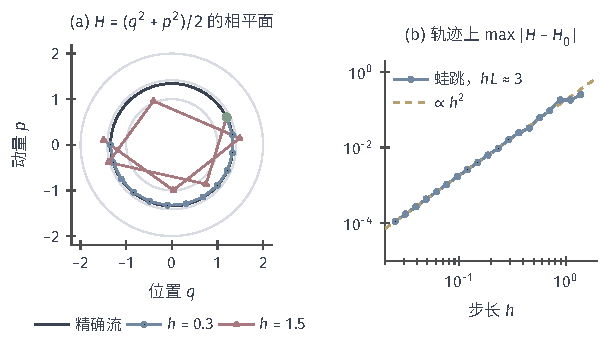
\includegraphics[width=102mm]{figures/03-optimization-evolution-and-signals/02-processes-and-trajectory-evolution/tikz/dtsp-hmc-leapfrog/figure.pdf}
  \caption{蛙跳积分的轨迹与能量误差。Hamilton量$H=(q^2+p^2)/2$，初值$(q,p)=(1.2,0.6)$（绿点）。(a)灰色为等能量圆，黑线为精确流，蓝线为$h=0.3$的$12$个蛙跳步，红线为$h=1.5$的$6$个蛙跳步；(b)总时间$hL\approx3$的轨迹上最大能量误差随步长的变化（双对数坐标），黄色虚线斜率为$2$。}
  \label{fig:dtsp-hmc-leapfrog}
\end{figure}

能量误差由Metropolis接受步校正。下面的定理对任意保体积的可微对合成立，蛙跳只是其中一例。

\begin{theorem}[对合提议的细致平衡]
  \label{thm:dtsp-hmc-balance}
  设$T$是相空间上可微、保体积的对合。以概率$\alpha(\bm z)=\min\{1,e^{H(\bm z)-H(T\bm z)}\}$从$\bm z$移到$T\bm z$、否则停在$\bm z$，所得核关于$\rho$满足细致平衡。
\end{theorem}

\begin{proof}
接受部分的密度流量为$\rho(\bm z)\alpha(\bm z)\propto\min\{\rho(\bm z),\rho(T\bm z)\}$。对任意有界可测$g$，作变量替换$\bm y=T\bm z$，由$T^2=I$及Jacobian绝对值为$1$，
\[
  \int g(\bm z,T\bm z)\min\{\rho(\bm z),\rho(T\bm z)\}\,\mathrm d\bm z=\int g(T\bm y,\bm y)\min\{\rho(T\bm y),\rho(\bm y)\}\,\mathrm d\bm y,
\]
即接受部分在交换出发点与到达点后不变。拒绝部分在对角线上，本身对称。
\end{proof}

由此得到\term{Hamilton蒙特卡洛}（Hamiltonian Monte Carlo）的一轮：保留位置$\bm q$，按$\mathcal N(\bm 0,\bm M)$重新抽取动量；从$(\bm q,\bm p)$出发走$L$个蛙跳步，翻转末端动量；以$\min\{1,e^{-\Delta H}\}$的概率接受末端位置，否则保留原位置\scite{pgm-sampling-neal2011}。动量刷新是对$\rho$的一次Gibbs更新，保持$\rho$；接受步由上面的定理保持$\rho$；二者复合仍保持$\rho$，但复合一般不再可逆。输出的位置序列按迭代编号构成一条离散时间Markov链，前面关于遍历、相关与误差评估的讨论全部适用。这里只用到确定性的常微分方程与它的离散化，不需要随机微积分。

使用时要记住它的成本与限制。每轮需要$L$次梯度计算，步长$h$决定接受率，轨迹长度$hL$决定能走多远，质量矩阵$\bm M$决定各方向的相对尺度。$U$须可微；多峰目标的峰间能量壁垒仍然难以跨越；步长若依赖当前状态，或提议不保持体积，接受率中还要加入相应的修正。Hamilton蒙特卡洛的目标是保持分布，能量并不沿轨迹下降，所以不能把它理解为一种更快的梯度下降。

\subsection{有限路径的重加权}
\label{sec:dtsp-path-reweighting}

\paragraph{整条路径的似然比}
重要性抽样也可以作用在整条路径上：手头有按一种规则生成的轨迹，想计算另一种规则下某个路径函数的平均。设$(X_0,\ldots,X_T)$在两个规律$P,Q$下关于同一参考测度分别有逐步条件密度$p_k(x_k\mid x_{<k})$与$q_k(x_k\mid x_{<k})$（$k=0$时为初始密度）。由条件密度的乘法公式，联合密度之比为
\begin{equation}
  L_T=\frac{\mathrm dQ}{\mathrm dP}(X_0,\ldots,X_T)=\prod_{k=0}^T\frac{q_k(X_k\mid X_{<k})}{p_k(X_k\mid X_{<k})},
  \label{eq:dtsp-path-likelihood-ratio}
\end{equation}
于是$\mathbb E_Q[F(X_{0:T})]=\mathbb E_P[L_TF(X_{0:T})]$。推导只用到联合分布的链式分解，不需要Markov性质。要求是：在$P$实际可能到达的每段历史上，凡$q_k>0$处都有$p_k>0$；$P$根本不会产生、而$Q$可能产生的路径，任何有限权重都无法补救。

似然比过程本身是一个鞅，这把本节与第~\ref{sec:dtsp-accumulation}节联系起来。在$P$下，
\[
  \mathbb E_P[L_{n+1}\mid\mathcal F_n]=L_n\int\frac{q_{n+1}(x\mid X_{\leq n})}{p_{n+1}(x\mid X_{\leq n})}p_{n+1}(x\mid X_{\leq n})\,\mathrm dx=L_n,
\]
最后一步用到$q_{n+1}$是概率密度且在$p_{n+1}$为零处也为零。所以$(L_n)$是均值为一的非负鞅。

\paragraph{策略轨迹的特例}
许多应用中，路径由“状态—行动”交替组成：$\tau=(s_0,a_0,s_1,a_1,\ldots,s_T)$，行动按概率核$\mu(a\mid s)$选择，下一状态按环境的转移核$P(s'\mid s,a)$产生。若要评价另一个行动规则$\pi(a\mid s)$，而初始分布与环境转移核不变，式~\eqref{eq:dtsp-path-likelihood-ratio}中环境因子在分子分母中相同而相消：
\begin{equation}
  \frac{p_\pi(\tau)}{p_\mu(\tau)}=\prod_{t=0}^{T-1}\frac{\pi(a_t\mid s_t)}{\mu(a_t\mid s_t)}.
  \label{eq:dtsp-policy-ratio}
\end{equation}
这意味着不知道环境转移概率也能计算权重。条件是$\pi(a\mid s)>0$时$\mu(a\mid s)>0$；若两种情形的环境不同，环境转移的比值必须保留。行动规则的设计与评价含义留给决策部分。

\paragraph{长路径的权重退化}
即使每一步的比值都温和，长路径的连乘也会失控。设$P$下各步增量独立服从$\mathcal N(0,1)$，$Q$下独立服从$\mathcal N(0.2,1)$，则每步对数比为$0.2x-0.02$，
\[
  \mathbb E_P[L_T^2]=\bigl(\mathbb E_Pe^{0.4X-0.04}\bigr)^T=e^{0.04T}.
\]
二阶矩随路径长度指数增长。另一方面，在$P$下$\log L_T$是均值$-0.02T$、方差$0.04T$的正态变量，所以$L_T\to0$几乎必然，而$\mathbb E_PL_T=1$始终成立：这正是第~\ref{sec:dtsp-martingale-limits}节“加倍或清零”所示的现象，期望被越来越少的路径携带。图~\ref{fig:dtsp-path-weight-degeneracy}中$N=1000$条路径的归一化有效样本比例在$T=50$时约为$0.15$，$T=200$时只剩约$0.025$，最大的一条路径一度占据总权重的三分之一以上。

\begin{figure}[htbp]
  \centering
  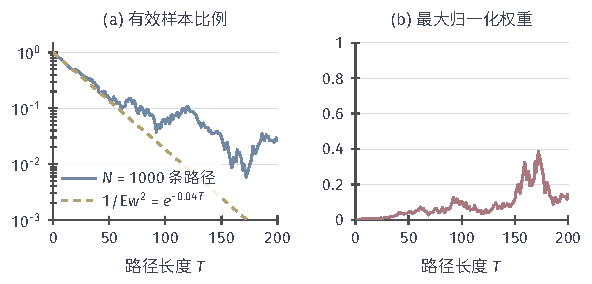
\includegraphics[width=100mm]{figures/03-optimization-evolution-and-signals/02-processes-and-trajectory-evolution/tikz/dtsp-path-weight-degeneracy/figure.pdf}
  \caption{路径权重的连乘退化。抽样规律下各步增量独立服从$\mathcal N(0,1)$，目标规律下服从$\mathcal N(0.2,1)$，$N=1000$条模拟路径（固定随机种子）。(a)归一化有效样本比例$(\sum_iL_T^{(i)})^2/(N\sum_i(L_T^{(i)})^2)$（纵轴对数刻度）与$1/\mathbb E_PL_T^2=e^{-0.04T}$；(b)最大归一化权重$\max_iL_T^{(i)}/\sum_iL_T^{(i)}$。}
  \label{fig:dtsp-path-weight-degeneracy}
\end{figure}

自归一化可以消去未知常数，却不能消除这种退化。逐步重采样把权重退化分摊到每一步，是粒子方法的核心，它与观测条件化一起属于信号与状态估计部分；连续时间路径的换测度需要额外的可积条件，在第~\ref{chap:continuous-time-stochastic-processes}章讨论。

\section{应用：带噪递推的稳定与收敛}
\label{sec:dtsp-stochastic-approximation}

最后一节把鞅累计、长期平均与确定性稳定性合起来，用于分析一类随机递推：每一步只能拿到带噪声的信息，却希望参数最终停在某个方程的根上。随机梯度下降是最常见的实例，但这里研究的对象是递推路径本身及其平均漂移，不是优化算法的目录；算法的设计与有限预算下的进展由优化部分讨论（第~\ref{chap:opt-stochastic-block}章），这里回答的是：随机轨迹为什么会稳定、在什么条件下收敛。

\subsection{随机求根与递推误差}
\label{sec:dtsp-root-finding}

\paragraph{只能观测带噪响应时的求根}
设想要找一个剂量$\theta$，使某种反应的平均强度恰好等于目标值。每做一次试验只能看到一个带噪声的读数，平均反应函数本身未知。形式上，有一个平均漂移$\overline h(\theta)=\mathbb E[H(\theta,Y)]$，我们只能在选定的$\theta$处取得$H(\theta,Y)$的一个随机实现，目标是找到$\overline h(\theta^\star)=0$的根。\term{随机逼近}（stochastic approximation）的基本递推是
\begin{equation}
  \bm\theta^{(n+1)}=\bm\theta^{(n)}+\alpha_n\bm H(\bm\theta^{(n)},Y_{n+1}),
  \label{eq:dtsp-robbins-monro}
\end{equation}
其中$\alpha_n>0$是步长\scite{math-robbins1951stochastic}。迭代编号用带括号的上标，与物理时间下标区分。按照Doob分解的思路，把每一步拆成三部分：
\begin{equation}
  \bm H(\bm\theta^{(n)},Y_{n+1})=\overline{\bm h}(\bm\theta^{(n)})+\bm\xi_{n+1}+\bm r_{n+1},
  \label{eq:dtsp-sa-decomposition}
\end{equation}
其中$\overline{\bm h}(\bm\theta^{(n)})$是平均漂移，$\bm\xi_{n+1}$满足$\mathbb E[\bm\xi_{n+1}\mid\mathcal F_n]=\bm 0$，是鞅差噪声，$\bm r_{n+1}$收集近似、截断或观测尚未平衡带来的偏差。分析的路线也随之确定：漂移部分用确定性稳定性处理，噪声部分用第~\ref{sec:dtsp-deviation}节的鞅工具处理，偏差部分须单独证明可以忽略。

三个例子说明这个框架有多宽。估计均值：$H(\theta,Y)=Y-\theta$，根为$\mu=\mathbb EY$；取$\alpha_n=1/(n+1)$，由归纳得$\theta^{(n)}=\frac1n\sum_{k\leq n}Y_k$，样本平均就是一种随机逼近。估计分位数：$H(\theta,Y)=q-\mathbb I\{Y\leq\theta\}$，平均漂移为$q-F(\theta)$，根是$q$分位数；每步只需一次比较，噪声有界。随机梯度：$\bm H(\bm\theta,Y)=-\nabla_{\bm\theta}\ell(\bm\theta,Y)$，在可交换微分与期望时平均漂移为$-\nabla L(\bm\theta)$，根是平均损失的驻点。

\paragraph{方程的根、计算误差与统计误差}
随机逼近收敛到的是所选方程$\overline h=0$的根。这个根是否就是我们真正关心的量，是建模问题，不是收敛问题：只有当模型正确、目标与方程的关系成立时，根才代表所需的参数。若递推运行在一组固定的数据上（例如对有限样本的平均损失做随机梯度），总误差可以分成两部分：迭代与该数据集上的根之间的计算误差，以及该根与总体目标之间的统计误差。本节只讨论前者。若数据在线到达、每步用一个新样本，样本数与迭代次数一起增长，计算误差与统计误差交织在一起，需要联合论证。统计误差的大小、效率与置信区间可参考\BookChapterRef{chap:statistical-inference}{卷四“统计推断”章}。

\subsection{步长、噪声与路径稳定}
\label{sec:dtsp-stepsizes}

\paragraph{两个步长条件的作用}
经典的递减步长条件是
\begin{equation}
  \sum_{n\geq0}\alpha_n=\infty,\qquad\sum_{n\geq0}\alpha_n^2<\infty.
  \label{eq:dtsp-robbins-monro-steps}
\end{equation}
两条分别对付两个敌人。第一条保证累计移动能力无限：若$\sum\alpha_n<\infty$，即使没有噪声，迭代也可能在到达根之前就“走不动了”，例如$\theta^{(n+1)}=\theta^{(n)}-\alpha_n\theta^{(n)}$的解是$\theta^{(0)}\prod(1-\alpha_k)$，在$\sum\alpha_k<\infty$时不趋于零。第二条控制累计噪声：噪声以$\alpha_n\bm\xi_{n+1}$的形式进入，若条件方差有统一上界$\sigma^2$，定理~\ref{thm:dtsp-weighted-martingale-sum}说明$\sum_n\alpha_n\bm\xi_{n+1}$几乎必然收敛，噪声的总影响有限。$\alpha_n=c/(n+n_0)^\gamma$在$c,n_0>0$、$\frac12<\gamma\leq1$时满足两条。仅有每一步方差有限还不够，因为方差可能随时间无界增长。

\paragraph{标量线性递推的收敛}
先在最简单的情形中把这两个条件与第~\ref{sec:dtsp-weighted-noise}节的几乎超鞅定理接起来。

\begin{theorem}[标量线性随机逼近]
  \label{thm:dtsp-scalar-sa}
  设$\theta^{(n+1)}=\theta^{(n)}+\alpha_n(b-a\theta^{(n)}+\xi_{n+1})$，其中$a>0$，$\mathbb E(\theta^{(0)})^2<\infty$，$\mathbb E[\xi_{n+1}\mid\mathcal F_n]=0$，$\mathbb E[\xi_{n+1}^2\mid\mathcal F_n]\leq\sigma^2$，确定步长满足式~\eqref{eq:dtsp-robbins-monro-steps}。则$\theta^{(n)}\to b/a$几乎必然。
\end{theorem}

\begin{proof}
记误差$e_n=\theta^{(n)}-b/a$，则$e_{n+1}=(1-a\alpha_n)e_n+\alpha_n\xi_{n+1}$，各$e_n$平方可积。$\alpha_n\to0$，舍去有限个初始步，可设$a\alpha_n\leq1$。展开平方并取条件期望，交叉项因$\xi$条件均值为零而消失：
\[
  \mathbb E[e_{n+1}^2\mid\mathcal F_n]=(1-a\alpha_n)^2e_n^2+\alpha_n^2\mathbb E[\xi_{n+1}^2\mid\mathcal F_n]\leq e_n^2-a\alpha_ne_n^2+\alpha_n^2\sigma^2.
\]
这正是式~\eqref{eq:dtsp-almost-supermartingale}，取$Z_n=e_n^2$、$\beta_n=0$、$b_n=\alpha_n^2\sigma^2$、$A_n=a\alpha_ne_n^2$。定理~\ref{thm:dtsp-almost-supermartingale}给出$e_n^2$几乎必然收敛到某个$L$，且$\sum_n\alpha_ne_n^2<\infty$。若某条路径上$L>0$，最终$e_n^2\geq L/2$，便有$\sum_n\alpha_ne_n^2\geq\frac L2\sum_n\alpha_n=\infty$，矛盾。所以$L=0$。
\end{proof}

证明清楚地显示了两个步长条件各自的位置：平方可和使$b_n$可求和，和发散使“累计下降有限”迫使误差趋零。取$a=1$、$b=\mu$就得到均值递推的收敛。

\paragraph{非线性情形：Lyapunov函数}
同一论证可以推广到非线性漂移，只要能找到一个沿平均漂移下降的“能量”。

\begin{theorem}[强单调漂移下的几乎必然收敛]
  \label{thm:dtsp-sa-lyapunov}
  设式~\eqref{eq:dtsp-robbins-monro}中$\bm r_{n+1}=\bm 0$，并存在$\bm\theta^\star$与常数$c>0$、$K<\infty$，使对所有$\bm\theta$，
  \[
    \begin{aligned}
      &\langle\bm\theta-\bm\theta^\star,\overline{\bm h}(\bm\theta)\rangle\leq-c\lVert\bm\theta-\bm\theta^\star\rVert_2^2,\\
      &\mathbb E\bigl[\lVert\bm H(\bm\theta^{(n)},Y_{n+1})\rVert_2^2\bigm|\mathcal F_n\bigr]\leq K\bigl(1+\lVert\bm\theta^{(n)}-\bm\theta^\star\rVert_2^2\bigr).
    \end{aligned}
  \]
  若$\mathbb E\lVert\bm\theta^{(0)}\rVert_2^2<\infty$且确定步长满足式~\eqref{eq:dtsp-robbins-monro-steps}，则$\bm\theta^{(n)}\to\bm\theta^\star$几乎必然。
\end{theorem}

\begin{proof}
令$Z_n=\lVert\bm\theta^{(n)}-\bm\theta^\star\rVert_2^2$。展开$\bm\theta^{(n+1)}-\bm\theta^\star=(\bm\theta^{(n)}-\bm\theta^\star)+\alpha_n\bm H$的平方并取条件期望，一次项中$\mathbb E[\bm H\mid\mathcal F_n]=\overline{\bm h}(\bm\theta^{(n)})$，于是
\[
  \mathbb E[Z_{n+1}\mid\mathcal F_n]\leq Z_n-2c\alpha_nZ_n+\alpha_n^2K(1+Z_n)=(1+K\alpha_n^2)Z_n+K\alpha_n^2-2c\alpha_nZ_n.
\]
由归纳，每个$Z_n$可积。定理~\ref{thm:dtsp-almost-supermartingale}（$\beta_n=b_n=K\alpha_n^2$，$A_n=2c\alpha_nZ_n$）给出$Z_n$收敛且$\sum\alpha_nZ_n<\infty$，再用$\sum\alpha_n=\infty$同前得极限为零。
\end{proof}

对随机梯度，第一条件就是平均损失的强凸性（$\overline{\bm h}=-\nabla L$，$L$为$c$强凸），第二条件允许梯度噪声的二阶矩随距离平方增长。两条都不能简单删去：没有漂移条件，迭代可能停在其他驻点或在多个吸引集之间徘徊；没有增长条件，噪声可能把迭代推到更远处，使有界性本身失去保证。一般非线性递推往往先要单独证明迭代几乎必然有界，再研究它被吸引到哪里，这正是下一小节的平均ODE方法。

\paragraph{固定步长与递减步长}
递减步长追求收敛；固定步长$\alpha_n\equiv\alpha$则保留对新观测的持续响应，代价是迭代不再收敛到一点，而在根附近持续波动。对均值递推，若观测独立同分布、方差为$\sigma^2$，误差满足$e_{n+1}=(1-\alpha)e_n+\alpha(Y_{n+1}-\mu)$，于是
\[
  \mathbb Ee_n=(1-\alpha)^ne_0,\qquad
  \operatorname{Var}(e_n)\to\frac{\alpha\sigma^2}{2-\alpha}.
\]
初始偏差几何地消失，留下与步长成正比的稳态方差。图~\ref{fig:dtsp-robbins-monro}比较三种步长：$\alpha_n=1/(n+1)$（样本平均）的均方误差为$1/n$；$\alpha_n=(n+1)^{-0.6}$下降得较慢；$\alpha=0.2$的均方误差很快停在$0.2/1.8=1/9$。更一般地，标量线性递推在$|1-a\alpha|<1$时，若噪声独立同分布、方差$v>0$，稳态方差为$\alpha^2v/(1-(1-a\alpha)^2)$。仅有条件方差的上界只能推出稳态误差的上界；要断言波动确实为正，还需要噪声非退化。

\begin{figure}[htbp]
  \centering
  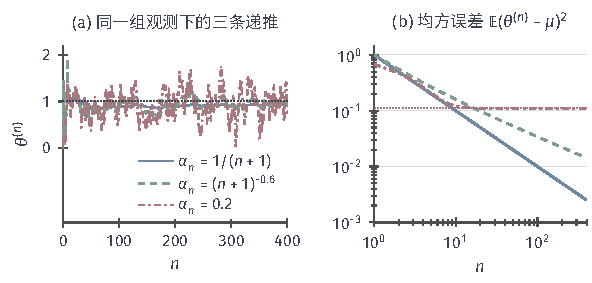
\includegraphics[width=100mm]{figures/03-optimization-evolution-and-signals/02-processes-and-trajectory-evolution/tikz/dtsp-robbins-monro/figure.pdf}
  \caption{均值估计的Robbins--Monro递推。观测独立服从$\mathcal N(1,1)$，$\theta^{(0)}=0$。(a)同一组模拟观测下三种步长的迭代路径；(b)由递推$m_{n+1}=(1-\alpha_n)^2m_n+\alpha_n^2$精确算出的均方误差（双对数坐标），点线为固定步长$0.2$的极限$1/9$。}
  \label{fig:dtsp-robbins-monro}
\end{figure}

\subsection{平均ODE与Markov噪声}
\label{sec:dtsp-ode-markov}

\paragraph{算法时钟与插值轨迹}
步长趋于零时，递推~\eqref{eq:dtsp-robbins-monro}的每一步都是对平均漂移的一个小Euler步，加上一点噪声。若用累计步长作为“时钟”，
\[
  \tau_0=0,\qquad\tau_n=\sum_{k<n}\alpha_k,
\]
并把点$(\tau_n,\bm\theta^{(n)})$用折线连起来，得到插值轨迹$\widehat{\bm\theta}(\tau)$，就可以把它与\term{平均ODE}（mean ODE）
\begin{equation}
  \dot{\bm\theta}(\tau)=\overline{\bm h}(\bm\theta(\tau))
  \label{eq:dtsp-mean-ode}
\end{equation}
的解比较。图~\ref{fig:dtsp-mean-ode-tracking}是一个二维线性例子：平均漂移$\overline{\bm h}(\bm\theta)=-\bm A\bm\theta$，$\bm A=\left(\begin{smallmatrix}0.5&-1\\1&0.5\end{smallmatrix}\right)$，平均ODE的解以$e^{-\tau/2}$的速度旋转着收缩。按迭代编号看，路径前段大步跳跃、后段挤成一团；按算法时间看，(b)中迭代的第一坐标紧紧跟着ODE解振荡衰减。

\begin{figure}[htbp]
  \centering
  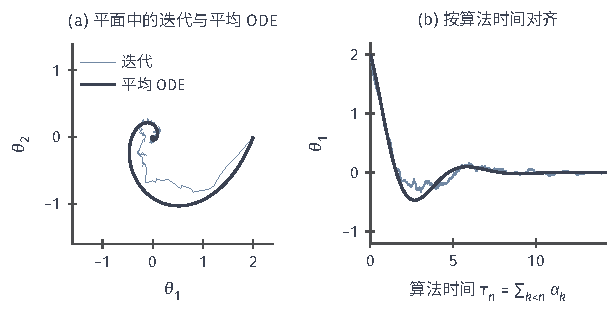
\includegraphics[width=104mm]{figures/03-optimization-evolution-and-signals/02-processes-and-trajectory-evolution/tikz/dtsp-mean-ode-tracking/figure.pdf}
  \caption{线性随机逼近与平均ODE。递推为$\bm\theta^{(n+1)}=\bm\theta^{(n)}+\alpha_n(-\bm A\bm\theta^{(n)}+\bm\xi_{n+1})$，$\bm A=\left(\begin{smallmatrix}0.5&-1\\1&0.5\end{smallmatrix}\right)$，$\bm\xi_n$独立服从$\mathcal N(\bm 0,0.64\bm I)$，$\alpha_n=0.6/(n+5)^{0.75}$，$\bm\theta^{(0)}=(2,0)$，共$3000$步（固定随机种子）。黑线为平均ODE的解$2e^{-\tau/2}(\cos\tau,-\sin\tau)$。(a)平面中的路径；(b)第一坐标对算法时间$\tau_n$。}
  \label{fig:dtsp-mean-ode-tracking}
\end{figure}

\term{ODE方法}（ODE method）把这一观察变成定理。它不要求每个随机增量都接近平均增量，只要求在任意长度固定的算法时间窗内，累计噪声和偏差最终可以忽略。一组常用的充分条件是：$\alpha_n\to0$且$\sum\alpha_n=\infty$；$\overline{\bm h}$局部Lipschitz；迭代几乎必然有界；对每个$T>0$，
\[
  \sup_{k\geq n,\ \tau_k-\tau_n\leq T}\Bigl\lVert\sum_{j=n}^{k-1}\alpha_j(\bm\xi_{j+1}+\bm r_{j+1})\Bigr\rVert_2\longrightarrow0\qquad\text{几乎必然}.
\]
鞅差部分的这一条件由定理~\ref{thm:dtsp-weighted-martingale-sum}保证：加权和几乎必然收敛，所以它的尾部在任何窗口上都一致趋于零。在这些条件下，插值轨迹在每个有限窗口上满足平均ODE的积分方程，只差一个一致趋零的残差；Grönwall不等式（见第~\ref{chap:ordinary-differential-equations}章）把残差转化为与ODE解的一致接近。这一步只连接了有限窗口内的轨迹；若平均ODE还有全局渐近稳定的平衡点$\bm\theta^\star$，并且它对迭代所在的紧集一致吸引，才能推出$\bm\theta^{(n)}\to\bm\theta^\star$\scite{math-borkar2008stochastic}。平均ODE若有多个吸引集，迭代可能落入其中任何一个；平均稳定也不意味着全局最优。

\paragraph{线性平均漂移的稳定条件}
对线性漂移$\overline{\bm h}(\bm\theta)=\bm b-\bm A\bm\theta$，平均ODE的误差满足$\dot{\bm e}=-\bm A\bm e$。由线性ODE的谱判据，$\bm A$的全部特征值实部为正时误差指数衰减。若对称部分$(\bm A+\bm A^{\top})/2$正定，欧氏能量$\frac12\lVert\bm e\rVert_2^2$本身就严格下降，因为反对称部分的二次型为零；图~\ref{fig:dtsp-mean-ode-tracking}的$\bm A$对称部分是$0.5\bm I$，属于这种情形。这一条件充分而不必要：$\bm A=\left(\begin{smallmatrix}1&10\\0&1\end{smallmatrix}\right)$的特征值都是$1$，对称部分却不定，欧氏误差可能先增大，换用由Lyapunov方程$\bm A^{\top}\bm P+\bm P\bm A=\bm Q$给出的二次型$\bm e^{\top}\bm P\bm e$才严格下降。

\paragraph{Markov观测与Poisson方程}
许多递推中，观测不是独立抽取的，而是来自一条Markov链：$\theta^{(n+1)}=\theta^{(n)}+\alpha_nH(\theta^{(n)},X_n)$，$X_n$以核$P$转移、不变分布为$\pi$。此时平均漂移是$\overline h(\theta)=\int H(\theta,x)\,\pi(\mathrm dx)$，但$H(\theta,X_n)-\overline h(\theta)$给定过去的条件均值一般不为零，它不是鞅差，第~\ref{sec:dtsp-weighted-noise}节的定理不能直接用。解决办法是第~\ref{sec:dtsp-ergodic-averages}节用过的Poisson方程：对固定的$\theta$求$g_\theta$，使
\[
  g_\theta-Pg_\theta=H(\theta,\cdot)-\overline h(\theta).
\]
代入后，相关误差被拆成一个鞅差和一个望远镜项：
\[
  H(\theta,X_n)-\overline h(\theta)=\underbrace{g_\theta(X_{n+1})-Pg_\theta(X_n)}_{\text{鞅差}}+\underbrace{g_\theta(X_n)-g_\theta(X_{n+1})}_{\text{相邻项相消}}.
\]
这里的Poisson方程是链的转移算子上的方程，与第~\ref{chap:partial-differential-equations}章空间区域上的Poisson边值问题名称相同，对象不同。

\begin{lemma}[有限链上的加权Poisson分解]
  \label{lem:dtsp-finite-poisson-sum}
  设$P$是有限状态上不可约、非周期的转移矩阵，迭代$\theta^{(n+1)}=\theta^{(n)}+\alpha_nH(\theta^{(n)},X_n)$始终位于紧集$K$，$H$在$K\times E$上有界且关于$\theta$一致Lipschitz，正步长单调递减且满足式~\eqref{eq:dtsp-robbins-monro-steps}。则$\sum_n\alpha_n[H(\theta^{(n)},X_n)-\overline h(\theta^{(n)})]$几乎必然收敛，从而它在任意有限算法时间窗上的尾和趋于零。
\end{lemma}

\begin{proof}
记$c_\theta=H(\theta,\cdot)-\overline h(\theta)$，$\pi(c_\theta)=0$。由定理~\ref{thm:dtsp-finite-convergence}，$g_\theta=\sum_{j\geq0}P^jc_\theta$一致绝对收敛，满足Poisson方程，并且存在常数$G,L_g$使$|g_\theta|\leq G$、$|g_\theta-g_{\theta'}|\leq L_g|\theta-\theta'|$（对$c_\theta-c_{\theta'}$用同样的几何界）。于是
\[
  \begin{aligned}
    \sum_{n\leq N}\alpha_nc_{\theta^{(n)}}(X_n)&=\sum_{n\leq N}\alpha_n\bigl[g_{\theta^{(n)}}(X_{n+1})-Pg_{\theta^{(n)}}(X_n)\bigr]\\
    &\quad+\sum_{n\leq N}\alpha_n\bigl[g_{\theta^{(n)}}(X_n)-g_{\theta^{(n)}}(X_{n+1})\bigr].
  \end{aligned}
\]
第一项是条件方差不超过$4G^2\alpha_n^2$的鞅差和，由定理~\ref{thm:dtsp-weighted-martingale-sum}收敛。第二项作分部求和，除去两个端点项外，中间各项为$\alpha_ng_{\theta^{(n)}}(X_n)-\alpha_{n-1}g_{\theta^{(n-1)}}(X_n)$，绝对值至多$G(\alpha_{n-1}-\alpha_n)+\alpha_{n-1}L_g|\theta^{(n)}-\theta^{(n-1)}|$；而$|\theta^{(n)}-\theta^{(n-1)}|\leq C\alpha_{n-1}$。前一部分由单调性望远镜求和，后一部分被$\sum\alpha_n^2$控制，端点项因$\alpha_n\to0$而消失。
\end{proof}

回到两状态链，取$H(\theta,x)=\mathbb I\{x=2\}-\theta$，递推估计长期拥堵比例$1/3$。由第~\ref{sec:dtsp-ergodic-averages}节，$g=(\mathbb I\{x=2\}-1/3)/0.3$，它不依赖$\theta$，参数变化带来的余项也就消失了。Poisson分解没有把相关样本变成独立样本，它把相关性的代价重新组织为一个放大了$1/(1-0.7)$倍的鞅噪声。一般状态空间或转移核本身依赖参数时，需要在迭代访问的区域上统一控制混合速度、Poisson解的矩界及其关于参数的正则性；这些条件使相关波动在算法时间上可以忽略，但不能把不稳定的平均根变成稳定根。

\subsection{快慢更新与迭代平均}
\label{sec:dtsp-two-timescale}

\paragraph{两个时间尺度}
有些算法同时更新两组变量，一组要跟踪另一组决定的目标。设
\[
  \begin{aligned}
    \bm u^{(n+1)}&=\bm u^{(n)}+\beta_n[\bm g(\bm u^{(n)},\bm v^{(n)})+\bm\eta_{n+1}],\\
    \bm v^{(n+1)}&=\bm v^{(n)}+\alpha_n[\bm f(\bm u^{(n)},\bm v^{(n)})+\bm\zeta_{n+1}],
  \end{aligned}
\]
两组步长都满足式~\eqref{eq:dtsp-robbins-monro-steps}，且$\alpha_n/\beta_n\to0$。在$\bm u$的时钟上看，$\bm v$几乎不动；在$\bm v$的时钟上看，$\bm u$已经跑到了它当前的平衡点。这启发了“冻结慢变量，替换快平衡”的分析：先对固定的$\bm v$研究快ODE$\dot{\bm u}=\bm g(\bm u,\bm v)$，设它有全局渐近稳定平衡$\bm u^\star(\bm v)$；再研究约化慢ODE$\dot{\bm v}=\bm f(\bm u^\star(\bm v),\bm v)$。这一论证成立需要一组条件同时满足：漂移局部Lipschitz；快平衡对每个慢状态存在、全局渐近稳定，吸引在访问的紧区域上一致，且$\bm u^\star$局部Lipschitz；约化慢ODE有全局渐近稳定平衡$\bm v^\star$；联合迭代几乎必然有界；两组鞅差的条件二阶矩在访问区域上统一有界。此时$(\bm u^{(n)},\bm v^{(n)})\to(\bm u^\star(\bm v^\star),\bm v^\star)$\scite{math-borkar2008stochastic}。

\begin{example}[快慢更新拆分同一个均值]
  \label{ex:dtsp-two-timescale}
  设$\mathbb E[Y_{n+1}\mid\mathcal F_n]=\mu$，取
  \[
    u^{(n+1)}=u^{(n)}+\beta_n(Y_{n+1}-u^{(n)}-v^{(n)}),\qquad
    v^{(n+1)}=v^{(n)}+\alpha_n(u^{(n)}-v^{(n)}).
  \]
  冻结$v$，快ODE$\dot u=\mu-v-u$的唯一稳定平衡为$u^\star(v)=\mu-v$；代入慢方程得$\dot v=\mu-2v$，所以$v^\star=\mu/2$，$u^\star(v^\star)=\mu/2$。快变量估计尚未被$v$解释的部分，慢变量调整两部分的分配。图~\ref{fig:dtsp-fast-slow-averaging}(a)取$\mu=2$、$\beta_n=(n+1)^{-0.6}$、$\alpha_n=(n+1)^{-0.9}$：$u+v$很快贴近$2$，而$u,v$各自缓慢地向$1$靠拢，$n=20000$时分别约为$0.993$与$1.011$。
\end{example}

尺度分离不能保证快平衡存在或稳定。两组步长同阶时，冻结论证不再成立，必须把两组变量当作一个联合系统分析。

\paragraph{迭代平均}
递减步长在“收敛快”和“噪声小”之间存在矛盾：步长大则跟得快、抖得厉害，步长小则抖得轻、走得慢。迭代平均提供了一个折中：用较大的步长（如$\alpha_n=n^{-\gamma}$，$\frac12<\gamma<1$）运行递推，同时报告迭代的累计平均$\overline{\bm\theta}^{(n)}=\frac1n\sum_{k\leq n}\bm\theta^{(k)}$。平均不改变目标，只削弱波动。

在标量线性情形可以看出为什么有效。由$e_{k+1}=e_k+\alpha_k(-ae_k+\xi_{k+1})$，有$ae_k=\xi_{k+1}+(e_k-e_{k+1})/\alpha_k$。对$k<n$求和并除以$n$，
\[
  a\,\overline e_n=\frac1n\sum_{k<n}\xi_{k+1}+\frac1n\sum_{k<n}\frac{e_k-e_{k+1}}{\alpha_k}.
\]
第一项是鞅差的平均，方差为$\sigma^2/n$量级；第二项经分部求和化为端点项与$\sum_k e_k(1/\alpha_k-1/\alpha_{k-1})$，在$e_k$按$\sqrt{\alpha_k}$的尺度缩小、$\gamma<1$等条件下，它比$1/\sqrt n$小。于是$\overline e_n$的方差约为$\sigma^2/(a^2n)$，与最优的步长$1/(an)$所能达到的相同，而不需要事先知道$a$。图~\ref{fig:dtsp-fast-slow-averaging}(b)对$a=1$的均值递推比较：$n=2000$时迭代本身的均方误差约为$6.3\times10^{-3}$，平均后约为$5.1\times10^{-4}$，几乎与样本平均的$1/n=5\times10^{-4}$重合。

\begin{figure}[htbp]
  \centering
  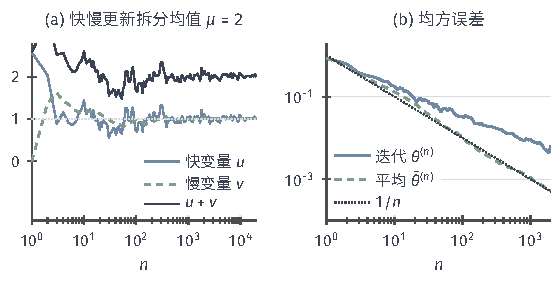
\includegraphics[width=94mm]{figures/03-optimization-evolution-and-signals/02-processes-and-trajectory-evolution/tikz/dtsp-fast-slow-averaging/figure.pdf}
  \caption{快慢更新与迭代平均（固定随机种子，横轴对数刻度）。(a)例~\ref{ex:dtsp-two-timescale}的一次运行，$Y$独立服从$\mathcal N(2,1)$，$\beta_n=(n+1)^{-0.6}$，$\alpha_n=(n+1)^{-0.9}$；点线为极限$1$。(b)均值递推$\theta^{(n+1)}=\theta^{(n)}+(n+1)^{-0.6}(Y_{n+1}-\theta^{(n)})$（$Y$独立服从$\mathcal N(1,1)$，$\theta^{(0)}=0$）的迭代与其累计平均在$200$次重复上的均方误差，点线为$1/n$。}
  \label{fig:dtsp-fast-slow-averaging}
\end{figure}

把这一观察推广为一般结论，需要在根附近对平均漂移作线性化（要求Jacobian的特征值实部为负）、噪声协方差收敛、步长满足$\frac12<\gamma<1$等条件，结论是平均迭代的缩放误差渐近正态，且协方差在一类估计中达到最小。这一结论关于估计效率与置信区间的统计含义属于统计推断部分；把递推在小步长下近似为随机微分方程的扩散逼近，留到第~\ref{chap:continuous-time-stochastic-processes}章，它们都不是本节主线结论的前提。

\section{本章小结}
\label{sec:dtsp-summary}

本章开头提出了几个问题：服务器从正常状态出发，若干步后拥堵的概率是多少；赌徒能否靠下注或停止规则改变期望收益；随时查看的累计误差最坏有多大；相关的采样序列怎样给出可信的积分；带噪更新怎样收敛到所需的根。回答这些问题用到了三类结构，它们回答不同的问题，可以同时出现在同一个过程上。

第一类是转移结构。一步转移核决定全部有限维分布，多步分布由核的复合给出（定理~\ref{thm:dtsp-chapman-kolmogorov}）。状态能否到达、是否返回、返回是否够快，分别由沟通类、常返性与平均返回时间刻画；不变分布是分布更新的不动点，细致平衡是验证它的便利充分条件。存在不变分布、它唯一、从任意初态收敛到它，是三件不同的事：有限不可约链保证前两件，加上非周期才保证第三件，并且收敛是几何的（定理~\ref{thm:dtsp-finite-convergence}）。

第二类是条件均值结构。Doob分解把任何适应累计量拆成可预测漂移与鞅（定理~\ref{thm:dtsp-doob-decomposition}）。可预测下注不能改变公平游戏的期望；有界停时的可选抽样保持期望，无界停时则需要控制、有限平均时间或一致可积等条件，加倍下注说明这些条件缺一不可。固定预算下，Doob最大不等式、Azuma与Freedman界控制整段运行的最大偏差，后者按实际的条件方差计费；向量自归一化界把同样的方法推广到可预测设计。无穷时间上，$L^1$有界的鞅几乎必然收敛，一致可积再保证期望保持，$L^2$有界给出均方收敛；有限时间的概率界与无穷时间的收敛是两类不同的结论。

第三类是长期平均。平稳性描述时间平移下规律不变；遍历定理说明不可约正常返链的时间平均收敛到不变分布下的平均，它不需要非周期性。相关样本的平均误差由积分自相关时间放大，中心极限定理借助Poisson方程把相关和归结为鞅。同一个公平随机游走同时是Markov链、鞅，并具有平稳增量，而它本身并不平稳，这个例子说明三类结构并不互斥。

两个应用检验了这些工具。采样积分中，独立Monte Carlo的误差按$n^{-1/2}$下降，方差与生成成本决定实际计算量；重要性抽样、控制变量、条件平均、对偶与分层在保持积分目标的同时改变方差，各有前提与代价；Metropolis--Hastings、Gibbs与Hamilton蒙特卡洛用细致平衡或保体积对合保持目标分布，再由遍历定理把时间平均当作积分，误差评估必须计入相关性；路径重加权的似然比是均值为一的鞅，长路径时权重退化。带噪求根中，步长和发散与平方可和分别保证到达与抑制噪声，几乎超鞅定理给出线性与强单调情形的完整证明，平均ODE方法在有界性与漂移正则性下把随机轨迹与确定性稳定性连接起来，Poisson方程处理Markov噪声，快慢尺度与迭代平均分别处理耦合更新与波动。

使用这些结论时，应分别核验三件事：递推或采样链本身是否稳定（有界、回返、混合），数值计算是否收敛到所设定的目标（步长与可积条件、遍历与方差条件），以及这个目标是否就是统计上需要的量（模型与识别）。前两件是本章的内容，第三件属于统计推断。下一章把时间改为连续：转移核变成半群与生成元，停止时刻可以取不可数多个值，噪声的累计需要随机积分，这些问题保留本章的结构，但需要新增路径正则性与可积性条件。

